\documentclass[a4paper,fleqn]{cas-sc}
\makeatletter
\@namedef{ver@authblk.sty}{}
\@namedef{ver@geometry.sty}{}
\@namedef{opt@geometry.sty}{left=1cm,right=1cm,top=2cm,bottom=2cm,paperwidth=20cm,paperheight=30cm}
\makeatother
\usepackage{tikz}
\usetikzlibrary{arrows.meta,positioning,shapes.multipart,fit,backgrounds,calc}
% Shared visual system for native TikZ manuscript figures.
% Keep semantic categories and typography stable; individual figures may vary geometry only.
\definecolor{pubInk}{HTML}{243746}
\definecolor{pubMuted}{HTML}{5F6B73}
\definecolor{pubBlueFill}{HTML}{DCEAF5}
\definecolor{pubTealFill}{HTML}{D9EEE9}
\definecolor{pubAmberFill}{HTML}{F7E7B7}
\definecolor{pubRedFill}{HTML}{F5D9D7}
\definecolor{pubSlateFill}{HTML}{E5EAED}
\definecolor{pubGreenFill}{HTML}{DDEBD7}

\tikzset{
  pub/base/.style={draw=pubInk, line width=0.55pt, rounded corners=2pt,
    align=center, font=\footnotesize, inner xsep=5pt, inner ysep=4pt},
  pub/input/.style={pub/base, fill=pubBlueFill},
  pub/representation/.style={pub/base, fill=pubTealFill},
  pub/process/.style={pub/base, fill=pubAmberFill},
  pub/physics/.style={pub/base, fill=pubGreenFill},
  pub/model/.style={pub/base, fill=pubSlateFill},
  pub/explanation/.style={pub/base, fill=pubAmberFill},
  pub/target/.style={pub/base, fill=pubRedFill},
  pub/arrow/.style={-{Stealth[length=2mm,width=1.35mm]}, draw=pubInk,
    line width=0.8pt},
  pub/flow/.style={-{Stealth[length=2.3mm,width=1.5mm]}, draw=pubInk,
    line width=1.05pt},
  pub/dashed/.style={pub/arrow, dashed, draw=pubMuted},
  pub/heading/.style={font=\footnotesize\bfseries, text=pubInk,
    align=center},
  pub/note/.style={font=\scriptsize, text=pubMuted, align=left},
  pub/legend/.style={font=\scriptsize, text=pubInk, anchor=west},
  % \scriptsize is reserved for legends, notes, and dense condition grids.
  % All semantic nodes and headings use the shared \footnotesize base.
  pub/condition/.style={pub/base, minimum width=1.05cm, minimum height=0.78cm,
    font=\scriptsize\bfseries},
  pub/train/.style={pub/condition, fill=pubBlueFill},
  pub/validation/.style={pub/condition, fill=pubAmberFill},
  pub/test/.style={pub/condition, fill=pubRedFill},
}

\usepackage[author={Ming Wu},date=date{},icon=Note,color=yellow]{pdfcomment}
\usepackage{graphicx}
\usepackage{svg}
\usepackage{textcomp,mathcomp,upgreek,outlines,physics}
\usepackage[version=4]{mhchem}
\usepackage{nicefrac,amsmath,mathtools,relsize}
\usepackage{algorithm,algpseudocode}
\usepackage{eqparbox,array}
\usepackage{xcolor}
% \usepackage[linesnumbered,ruled,vlined]{algorithm2e}
\usepackage{amssymb}
% \usepackage{natbib}
\usepackage[utf8]{inputenc}
\usepackage{booktabs,longtable}
\usepackage{calc}
\usepackage{bookmark}
\usepackage{hyperref}
\usepackage{authblk}%author
\usepackage{lipsum}
\usepackage{lineno}
\usepackage{filecontents}
\linenumbers
% \usepackage{siunitx}

\newcommand{\tightlist}{}
\newcommand{\micron}{$\mathrm{\(\upmu\)m}$ }

% SVG
% \svgsetup{inkscapeversion=1,inkscapepath=./figures/, inkscape=force, inkscapedpi=600, inkscapearea=page, inkscapeformat=pdf, inkscapelatex=false}
\svgsetup{inkscapeversion=1,inkscapepath=./figures/, inkscapedpi=600, inkscapearea=page, inkscapelatex=false, extractformat={pdf,eps},clean=true}

% PDF comments
\pdfcommentsetup{final}


% subsubsubsection
\newcommand{\subsubsubsection}[1]{\paragraph{#1}\mbox{}\\}
\setcounter{secnumdepth}{4}
\setcounter{tocdepth}{4}

\newcommand{\subsubsubsubsection}[1]{\paragraph{#1}\mbox{}\\}
\setcounter{secnumdepth}{5}
\setcounter{tocdepth}{5}

%% style
\usepackage[left=1cm,right=1cm,top=2cm,bottom=2cm,paperwidth=20cm,paperheight=30cm]{geometry}% Easy control of page dimensions
% paperwidth=100cm,paperheight=300cm
\usepackage{changepage}%Alter page layout
\usepackage[font=small,labelfont=bf]{caption} %make Figure in bold, and make the caption content small.

\hypersetup{
  colorlinks   = true, %Colours links instead of ugly boxes
  urlcolor     = blue, %Colour for external hyperlinks
  linkcolor    = blue, %Colour of internal links
  citecolor   = blue  %Colour of citations
}

\newcommand{\MW}[1]{\textcolor{blue}{\textbf{(MW: #1)}}}
\newcommand{\MV}[1]{\textcolor{magenta}{\textbf{(MV: #1)}}}
\newcommand{\MA}[1]{\textcolor{orange}{\textbf{(MA: #1)}}}
\newcommand{\BM}[1]{\textcolor{purple}{\textbf{(BM: #1)}}}
\newcommand{\BG}[1]{\textcolor{violet}{\textbf{(BG: #1)}}}

\providecommand{\keywords}[1]
{
  \small
  \textbf{\textit{Keywords---}} #1
}

\newcommand*{\matr}[1]{\mathbfit{#1}}
\newcommand*{\tran}{^{\mkern-1.5mu\mathsf{T}}}
\newcommand*{\conj}[1]{\overline{#1}}
\newcommand*{\hermconj}{^{\mathsf{H}}}

\newcommand*{\Register}{\textsuperscript{\tiny\textregistered}}

\newcommand*{\figref}[2][]{% \figref [<sub caption>][<figure label>]
  \hyperref[{#2}]{%
    Fig.~\ref*{#2}%
    \ifx\\#1\\%
    \else
      \,($\mathrm{#1}$)%
    \fi
  }%
}
\newcommand*{\secref}[1]{% \secref [ref]
  \hyperref[{#1}]{%
    Section~\ref*{#1}%
  }%
}

\newcommand*{\refcite}[1]{
  \hyperref[{#1}]{%
    Ref.~\cite{#1}%
  }%
}

\newcommand*{\apref}[1]{
  \hyperref[{#1}]{%
    Appendix~\ref*{#1}%
  }%
}
\newcommand*{\tableref}[1]{%
  \hyperref[{#1}]{%
    Table~\ref*{#1}%
  }%
}
\newcommand*{\equationref}[1]{%
  \hyperref[{#1}]{%
    Equation~\ref*{#1}%
  }%
}


\newcommand*{\algoref}[1]{%
  \hyperref[{#1}]{%
    Algorithm~\ref*{#1}%
  }%
}

\newcommand{\SI}[2]{${#1} \mskip3mu \mathrm{#2}$}

% Algorithms
% Comments
\algrenewcommand{\algorithmiccomment}[1]{\hfill// \eqparbox{COMMENT\thealgorithm}{#1}}
\algnewcommand{\LongComment}[1]{\hfill// \begin{minipage}[t]{\eqboxwidth{COMMENT\thealgorithm}}#1\strut\end{minipage}}
% Fun and Var
\definecolor{functionColor}{RGB}{255, 199, 6}
\definecolor{casblue}{RGB}{0, 112, 155}
% \newcommand{\var}[1]{\text{\texttt{#1}}}
\newcommand{\func}[1]{\textcolor{BlueViolet}{\texttt{#1}}}
% \newcommand{\func}[1]{\text{\textsl{#1}}}
% ForEach
\algnewcommand\algorithmicforeach{\textbf{for each}}
\algdef{S}[FOR]{ForEach}[1]{\algorithmicforeach\ #1\ \algorithmicdo}
% Sections
\newcounter{phase}[algorithm]
\newlength{\phaserulewidth}
\newcommand{\setphaserulewidth}{\setlength{\phaserulewidth}}
\newcommand{\phase}[1]{%
  \vspace{-1.25ex}
  % Top phase rule
  \Statex\leavevmode\llap{\rule{\dimexpr\labelwidth+\labelsep}{\phaserulewidth}}\rule{\linewidth}{\phaserulewidth}
  \Statex\strut\refstepcounter{phase}\textit{Phase~\thephase~--~#1}% Phase text
  % Bottom phase rule
  \vspace{-1.25ex}\Statex\leavevmode\llap{\rule{\dimexpr\labelwidth+\labelsep}{\phaserulewidth}}\rule{\linewidth}{\phaserulewidth}}
\makeatother
\setphaserulewidth{.7pt}

% \setcitestyle{square,numbers,sort&compress}
\graphicspath{{./images}}
\hypersetup{hidelinks}
\usepackage{url}
\usepackage{upgreek}

%%%Author macros
\def\tsc#1{\csdef{#1}{\textsc{\lowercase{#1}}\xspace}}
\tsc{WGM}
\tsc{QE}
\tsc{EP}
\tsc{PMS}
\tsc{BEC}
\tsc{DE}
%%%

\begin{document}
\let\WriteBookmarks\relax
\def\floatpagepagefraction{1}
\def\textpagefraction{.001}
\shorttitle{Multimodal signal processing for grinding roughness}
\shortauthors{M. Wu and J. Zha}

\title [mode = title]{Physics-aware multimodal acoustic-emission and vibration signal processing for interpretable surface roughness prediction in grinding}
\author[1,2,3]{Ming Wu}[
    orcid=0000-0002-3582-4881
]
\ead{ming.wu@kuleuven.be}

\author[4,5]{Jun Zha}
\ead{jun_zha@xjtu.edu.cn}
\cormark[1]

\affiliation[1]{organization={Department of Mechanical Engineering, KU Leuven}, addressline={3001 Leuven, Belgium}}
\affiliation[2]{organization={Flanders Make@KU Leuven}, addressline={3001 Leuven, Belgium}}
\affiliation[3]{organization={Department of Computer Science, KU Leuven}, addressline={3001 Leuven, Belgium}}
\affiliation[4]{organization={School of Mechanical Engineering, Xi'an Jiaotong University}, addressline={Xi'an 710049, China}}
\affiliation[5]{organization={Suzhou Academy of Xi'an Jiaotong University}, addressline={Suzhou 215123, China}}

\cortext[1]{Corresponding author}

% Research highlights
\begin{highlights}
    \item LOGO evaluation spans 25 reconstructable and two archival model variants.
    \item Auditable tree ensembles on dB-z descriptors yield low point-estimate error.
    \item SHAP and Grad-CAM associate predictions with plausible frequency bands.
    \item Uncertainty analysis reveals calibration failures on unseen conditions.
    \item Feature-precomputed inference timing quantifies model latency trade-offs.
\end{highlights}

\begin{keywords}
    Grinding surface roughness \sep
    Acoustic emission \sep
    Vibration \sep
    Spectrogram \sep
    Wavelet scattering \sep
    Auditable machine learning \sep
    Explainable AI \sep
    Industrial informatics
\end{keywords}

\begin{abstract}
Pass-end prediction of grinding surface roughness (\(R_a\)) from signals
acquired in process may support
earlier detection of surface-quality deviations, but small condition-structured
datasets make model selection, validation, and interpretation difficult. This
study benchmarks 27 model variants across 38 input configurations using
strict leave-one-condition-out cross-validation over 16 grinding conditions.
Inputs include process parameters, scalar signal features, full-resolution dB
spectrograms, per-sample-standardised dB (dB-z) spectrograms, log-mel
spectrograms, and two-dimensional wavelet-scattering descriptors.

The leading observed point-estimate group comprises random forests on fused
acoustic-emission and vibration dB-z and log-mel descriptors. The
reproducible current fixed dB-z pipeline gives \(0.0210~\upmu\)m, while
cache-matched inner-grouped reruns give \(0.0207~\upmu\)m for dB-z and
\(0.0206~\upmu\)m for log-mel. Their mean errors are nearly tied, but the
nested maximum fold errors are 0.1402 and 0.2061~\(\upmu\)m, respectively,
so dB-z has better observed worst-condition robustness. Historical canonical ranking artifacts
(0.0200 and 0.0201~\(\upmu\)m) are retained for provenance and the planned
post-selection comparison, not as evidence of a unique winner. For the
current fixed dB-z model, the median fold MAE is \(0.0093~\upmu\)m but the
maximum is \(0.1478~\upmu\)m on Condition~7, exposing substantial unseen-condition
tail risk. These differences are also close to the available measurement
uncertainty scale. In the planned post-selection family of 14
Holm--Bonferroni-corrected Wilcoxon tests, only the comparison with the
implementation-specific historical shallow MLP remains significant after
correction; a corrected whole-condition-validation MLP sensitivity remains
worse but is not part of that historical family. Vibration alone nearly
matches the fused RF, so the observed mean-level contribution of AE is small.

TreeSHAP, ridge coefficients, and Grad-CAM identify model-associated
frequency regions, but sensor-response limitations preclude causal
interpretation of high-frequency AE attributions. For a separately regenerated
ResNetVibCNN checkpoint set with deterministic MAE of \(0.0443~\upmu\)m,
nominal MC-dropout epistemic-band coverage is 50.2\%; out-of-bag-scaled intervals for a separate 15-condition RF uncertainty variant also
under-cover difficult conditions, including
Condition~7. The results support auditable random forests with dB-z or
log-mel pass-level spectral descriptors as strong observed baselines in this
dataset, rather than general superiority over deep learning. The comparison
is post-selection and non-nested, and full-pass feature aggregation does not
establish within-pass or closed-loop readiness.
\end{abstract}

\maketitle
\section{Introduction}\label{introduction}

Grinding is widely used as a precision finishing process when tight dimensional tolerances, controlled surface texture, and stable near-surface properties are required for high-value components. The arithmetic mean roughness \(R_a\) remains one of the most commonly reported descriptors of ground-surface quality \cite{Brinksmeier2006,Jawahir2011}, although it represents only part of the broader surface-integrity response. Surface roughness can affect fatigue performance \cite{Novovic2004}, tribological behaviour \cite{Brinksmeier2006}, and coating adhesion or tolerance compliance \cite{Jawahir2011}, particularly when the component operates under cyclic loading or sliding contact. Stylus profilometry provides accurate post-process roughness measurement, but it is typically offline, local, and too slow for immediate corrective action in a control loop. These constraints motivate in-process or near-real-time prediction of \(R_a\) from machine signals acquired during grinding.

Acoustic emission (AE), vibration, and process parameters provide complementary information on the grinding process. AE signals contain high-frequency elastic-wave components that are associated with localized contact phenomena \cite{Dornfeld1992}, such as grain--workpiece interaction, rubbing, grit fracture, wheel loading, and micro-fracture \cite{Teti2010}. Vibration signals describe the dynamic response of the wheel--workpiece--machine system, including spindle and wheel modes \cite{Altintas2004}, chatter-related behaviour \cite{Quintana2011}, and structural transmission through the machine tool \cite{Hassui2003}. Process parameters such as wheel speed, workpiece speed, and depth of cut provide additional regime-level context because the same sensor amplitude or spectral pattern may have different implications under different operating conditions. Thus, AE and vibration are physically complementary: AE is more sensitive to localized high-frequency contact phenomena, whereas vibration captures system-level dynamics. At the same time, AE interpretation must remain sensor-aware because measured high-frequency content is shaped by the sensor bandwidth, couplant, mounting path, and transfer function.

Before deep learning became common in manufacturing monitoring, roughness and process-state prediction were usually based on engineered signal descriptors. Time-domain features such as RMS, variance, skewness, and kurtosis have been widely applied to tool state classification \cite{Byrne1995}, often in combination with frequency-band energy \cite{Antoni2006} or wavelet-based descriptors and process parameters \cite{Teti2010}. These descriptors have been mapped to surface roughness using linear regression or shallow neural networks \cite{Benardos2003}, and to tool condition and chatter using support vector regression \cite{Ozel2005} or random forests and boosted-tree models \cite{Wuest2016}. Such approaches are compact, relatively data-efficient, and easier to audit than high-capacity neural networks. However, manually selected scalar features may miss local time--frequency structures, and many studies have been restricted to one signal representation or one model family, making it difficult to separate the effect of feature design from the effect of the regression model.

Recent manufacturing-monitoring studies have increasingly adopted convolutional neural networks and residual encoders \cite{Wang2018}, spectrogram-based CNNs and attention mechanisms \cite{Khan2018}, and transformers or graph-based models \cite{Lei2020}. These methods are attractive because time--frequency representations can be processed directly, allowing local spectral patterns to be learned without complete reliance on handcrafted feature definitions. Multimodal fusion can also combine AE, vibration, force, power, process parameters, and engineered descriptors at data, feature, or decision level \cite{Khaleghi2013}. When the training data are large, diverse, and representative of the future operating range, such models can provide accurate predictions. Nevertheless, their performance must be assessed under validation protocols that reflect the intended deployment scenario, particularly when the experimental dataset is small and condition-structured.

Grinding experiments are often expensive, machine-specific, and limited in the number of process conditions that can be tested. Repeated grinding passes collected under the same condition are not independent in the same sense as randomly sampled observations, because they share wheel state, process parameters, material context, machine dynamics, and measurement setup. Ordinary random train--test splits or random \(K\)-fold cross-validation can therefore leak condition identity from training to test data and yield overly optimistic estimates of generalization to unseen grinding regimes. Related concerns have been reported for cross-validation during model selection \cite{varma2006bias} and for structured datasets requiring grouped validation \cite{Roberts2017}. In addition, deep networks may be sensitive to initialization, architecture selection, validation fold, hyperparameter tuning, and post-selection when the number of independent experimental conditions is small. Their larger parameter counts and preprocessing requirements may also complicate low-latency monitoring, while learned features can be difficult to diagnose when a specific held-out condition fails. These limitations do not imply that deep learning is unsuitable for grinding monitoring; rather, they indicate that deep-learning models should be compared with transparent and more auditable baselines under identical grouped validation.

A complementary strategy is to encode domain structure before learning. Regularized linear models, such as ridge regression, provide signed coefficients after feature standardization and permit direct inspection of feature-level associations \cite{Hoerl1970}. Tree ensembles are not fully transparent, but random forests \cite{Breiman2001} and gradient-boosted trees \cite{Friedman2001} are more auditable than many deep architectures. Split statistics and permutation importance can be computed via XGBoost \cite{Chen2016} or LightGBM \cite{Ke2017}, while localized attributions are available through TreeSHAP analysis \cite{Lundberg2020}. Physics-aware representations can also reduce the burden placed on the supervised model by compressing sensor data into structured descriptors, including wavelet-scattering transforms \cite{mallat2012group} and heuristic process or sensor indicators \cite{Anden2014}. Such representations may be data-efficient and stable in small manufacturing datasets, but their advantage must be demonstrated rather than assumed. A fair assessment requires that they be tested against evaluated deep-learning baselines under the same folds, metrics, and model-selection constraints.

Prior grinding roughness studies have often lacked at least one of the following elements: strict condition-level validation, systematic comparison of signal representations, auditable and deep models evaluated under identical folds, statistical testing at the condition level, seed sensitivity analysis, uncertainty calibration under grouped condition shift, condition-level failure analysis, or latency and model-footprint comparison. As a result, it remains unclear whether physics-motivated and more auditable models can provide competitive \(R_a\) prediction when the test condition is entirely unseen. The central question addressed in this work is therefore: can directly inspectable linear models and tree ensembles supported by post-hoc attribution provide competitive \(R_a\) prediction relative to evaluated neural baselines under strict leave-one-condition-out validation, while exposing uncertainty or failure modes under grouped condition shift?

This study investigates in-process \(R_a\) prediction from multimodal AE, vibration, and process-parameter data collected during grinding. The dataset contains 319 valid grinding passes grouped into 16 grinding conditions generated by a fractional 16-condition design; it is not a full \(4 \times 4 \times 4\) factorial experiment. Generalization is assessed by strict leave-one-condition-out cross-validation with 16 folds, so each test fold corresponds to a previously unseen grinding condition. The benchmark inventory contains 25 exactly reconstructable model variants and two archival variants with incomplete resolved-configuration provenance across 38 input configurations, covering process parameters, time-domain statistics, handcrafted and physics-informed features, dB spectrograms, dB-z descriptors, and two-dimensional wavelet-scattering representations for AE and vibration. A directly inspectable ridge baseline, auditable tree ensembles with post-hoc attribution, and a separate shallow neural baseline are compared with evaluated deep-learning architectures, including ResNet-style spectrogram CNNs, multimodal fusion CNNs, bilinear fusion, trajectory CNN, graph-fusion, TabTransformer, and attention-based regressors. Explainability is examined using ridge coefficients, TreeSHAP, and Grad-CAM, but the resulting attributions are interpreted as physically plausible associations rather than causal proof. Uncertainty is evaluated under full leave-one-condition-out validation using MC-dropout and RF OOB/tree-variance intervals, with emphasis on under-coverage and condition-level outliers rather than on solved calibration. Finally, feature-precomputed model-inference timing and model-footprint analyses are reported separately from full end-to-end deployment latency, which would also require the acquisition window, STFT/dB-z/log-mel computation, feature scaling, communication overhead, and edge-hardware testing to be considered.

In the present benchmark, random forests trained on pass-level fused AE and vibration dB-z or log-mel descriptors form the leading observed point-estimate group. This result should be interpreted cautiously. The primary planned statistical comparison establishes conclusive superiority only over the shallow MLP baseline, while a current fixed-setting five-seed analysis gives the same qualitative ordering for selected baselines but does not reproduce the historical tuned checkpoints. In addition, the best MAE is close to the manufacturer-quoted repeatability of the profilometer, and raw trace-level repeatability or gauge R\&R data are unavailable. Consequently, sub-\(0.005\)--\(0.010~\upmu\)m ranking differences are not treated as practically meaningful. The intended contribution is therefore not a general rejection of deep learning, but a condition-level, representation-aware, and measurement-conscious comparison of physics-aware machine-learning strategies for interpretable grinding roughness prediction.

\section{Related work}\label{related-work}

\subsection{Grinding roughness monitoring with AE and vibration}\label{rw:ae-vibration}

Grinding differs from many cutting processes because material removal is distributed over a large number of abrasive grains with stochastic protrusion heights, local rubbing, ploughing, chip formation, grain wear, and possible thermal damage. Surface roughness is therefore affected by controllable process parameters \cite{malkin2008grinding} and evolving wheel--workpiece interaction mechanisms \cite{Brinksmeier2006}. Reviews of surface integrity in material-removal processes have emphasized that topography, residual stress, microstructural alteration, and thermal-mechanical effects jointly determine functional performance, which makes roughness prediction a useful but incomplete indicator of final quality \cite{Jawahir2011}. In-process sensing is consequently attractive because it can provide information on process evolution before offline metrology is available.

AE has been used in machining monitoring because high-frequency stress waves are generated by localized contact \cite{Dornfeld1992}, micro-fracture, and rubbing interactions \cite{Teti2010}. In grinding, AE is often sensitive to events near the wheel--workpiece interface and can respond to wheel loading, dressing condition, contact initiation, burn-related changes, and changes in removal regime. However, AE signals are filtered by the sensor, couplant, mounting path, fixture, and machine structure. Interpretation of frequency-localized attributions therefore requires caution, especially when model explanations emphasize regions above the nominal flat-response band of the sensor.

Vibration sensing provides a complementary route because it measures the dynamic response of the machine-tool structure rather than only localized high-frequency activity. Chatter, spindle modes, and machine compliance can leave signatures in vibration spectra \cite{Altintas2004}, which can also reveal wheel wear or imbalance \cite{Quintana2011}. Empirical grinding studies have shown that vibration features can correlate with surface roughness in cylindrical grinding, supporting the use of vibration as a roughness-prediction modality \cite{Hassui2003}. Because AE and vibration emphasize different frequency ranges and physical pathways, their fusion can reduce reliance on a single sensor and can expose disagreements between local contact activity and system-level dynamics.

\subsection{Signal representations for grinding monitoring}\label{rw:representations}

Feature engineering in grinding and machining monitoring has typically combined time-domain, frequency-domain, and time--frequency descriptors. Time-domain features such as RMS, variance, skewness, kurtosis, peak-to-peak value, crest factor, and envelope statistics are compact and inexpensive. Frequency-domain features such as band power, dominant-frequency amplitude, spectral centroid, and spectral kurtosis can isolate energy changes associated with dynamic modes or impulsive events \cite{Antoni2006}. Wavelet-based features have also been used because grinding and AE signals are non-stationary and may contain transient events that are not well represented by pass-level averages alone \cite{Teti2010}.

Spectrograms provide a direct two-dimensional representation of temporal and spectral variation. In deep-learning pipelines, they allow CNNs to learn local time--frequency patterns using architectures originally developed for images or audio-like signals. Log-frequency, log-spectrogram, and mel descriptors compress or reweight the spectrum and can reduce sensitivity to narrow high-frequency fluctuations while preserving broad-band energy trends. In the present grinding context, these descriptors should be treated as engineered spectral summaries rather than as psychoacoustic models, because the mel scale was not designed for AE physics. Their value is empirical and representational: they provide compact spectral summaries that may be useful when the number of grinding passes is limited.

Wavelet-scattering transforms offer another compromise between handcrafted features and learned deep representations. Scattering networks use cascaded wavelet modulus operators to generate translation-stable and deformation-stable descriptors without supervised learning of convolutional filters \cite{mallat2012group}, as demonstrated on various signal tasks \cite{Anden2014}. This property is useful when the dataset is too small to estimate many convolutional parameters reliably. In grinding, two-dimensional scattering descriptors computed from AE or vibration maps can provide structured multi-scale summaries while preserving more local information than scalar pass-level statistics. Their disadvantage is that the representation is fixed and may not match the most discriminative frequency bands for a particular machine, wheel, sensor, or material.

\subsection{Transparent and classical machine-learning models}\label{rw:transparent-ml}

Classical machine-learning approaches remain relevant for surface roughness prediction because many manufacturing datasets are small, structured, and tabular after feature extraction. Linear regression and shallow neural networks have been widely used for machining roughness prediction \cite{Benardos2003}, while support vector regression \cite{Ozel2005} and random forests or boosted trees \cite{Wuest2016} are preferred when process parameters and sensor summaries are available. These models are often easier to train and tune than deep networks and can be more stable when the number of experimental conditions is limited.

Ridge regression is a useful baseline because it regularizes correlated predictors and produces coefficients that can be inspected after standardization \cite{Hoerl1970}. A ridge model is not guaranteed to be physically correct, but it can reveal whether predictions rely on plausible process parameters or frequency bands. Random forests \cite{Breiman2001} and gradient-boosted trees \cite{Friedman2001} can model nonlinear interactions and threshold effects without requiring a large neural architecture. XGBoost \cite{Chen2016} and LightGBM \cite{Ke2017} provide efficient implementations of gradient-boosted decision trees and are frequently competitive on structured tabular tasks. Recent empirical comparisons have also shown that tree-based methods remain strong baselines for tabular datasets, especially when data are limited \cite{shwartz2022tabular} or heterogeneous \cite{grinsztajn2022tree}. This evidence supports the inclusion of tree ensembles in grinding roughness benchmarks, but it does not imply that they will always outperform deep models.

\subsection{Deep learning and multimodal fusion for manufacturing monitoring}\label{rw:deep-fusion}

Deep learning has been widely studied for manufacturing monitoring \cite{Wang2018}, machine fault diagnosis \cite{Khan2018}, and system health management \cite{Lei2020} because learned representations can reduce manual feature design. CNNs are suited to spectrograms and other two-dimensional maps; recurrent or temporal-convolutional models can process sequences; attention mechanisms and transformers can learn interactions across time steps, features, or modalities; and graph-based models can encode relationships among sensors, process variables, or operating conditions. These methods are especially appealing when the training set covers the expected operating range and when the test distribution resembles the training distribution.

Multimodal fusion is relevant because manufacturing sensors rarely provide independent or complete information. General sensor-fusion literature distinguishes data-level, feature-level, decision-level, and hybrid fusion strategies \cite{Khaleghi2013}. In grinding, feature-level fusion can combine AE descriptors, vibration descriptors, and process parameters before regression. Deep fusion architectures can learn modality-specific encoders before concatenation, bilinear interaction, attention pooling, or graph-based aggregation. Such models can capture cross-modal relations, but they also introduce additional parameters and design choices. When only several hundred passes are available, the gain from flexible fusion must be weighed against the increased risk of fold-specific tuning and unstable post-selection.

For this reason, deep-learning results in small manufacturing datasets should be interpreted as conditional on the experimental design, validation protocol, and tuning procedure. A ResNet-style spectrogram CNN may be appropriate when local time--frequency motifs generalize across conditions, whereas a pass-level tree ensemble may be preferable when the dominant information is contained in broad spectral summaries and process-regime variables. The present work therefore treats deep models as evaluated baselines, not as a class to be rejected. The comparison is intended to identify which representation--model combinations generalize under strict condition-level exclusion.

\subsection{Validation protocols, model-selection bias, and measurement uncertainty}\label{rw:validation}

Validation design is central in grinding roughness prediction because repeated passes within a condition share process settings and machine context. If such passes are split randomly, models may learn condition identity rather than condition-invariant roughness mechanisms. Similar issues have been discussed in cross-validation studies showing that model selection can produce biased performance estimates when tuning and evaluation are not separated \cite{varma2006bias}, leading to optimistic assessments \cite{Cawley2010}, and that structured data require validation folds aligned with the grouping structure \cite{Roberts2017}. Leave-one-condition-out validation is therefore more stringent than random K-fold validation for this manuscript because each test fold corresponds to a grinding condition unseen during training.

Condition-level validation also changes the interpretation of statistical testing. When the effective unit of generalization is the condition, fold-level errors are more relevant than pass-level errors for comparing models. This reduces the apparent sample size from hundreds of passes to 16 held-out conditions and makes strong statistical claims harder to justify. The present manuscript therefore distinguishes point-estimate ranking from inferential conclusions: the best point-estimate model is a random forest on fused AE and vibration dB-z descriptors, but the planned statistical comparison supports conclusive superiority only over the shallow MLP baseline.

Measurement uncertainty further constrains interpretation. If the best MAE is close to the manufacturer-quoted profilometer repeatability or below the expanded uncertainty scale, then very small differences between models may reflect metrology noise, trace placement, surface heterogeneity, or repeatability limits rather than meaningful predictive improvement. The absence of raw trace-level repeatability and gauge R\&R prevents a full measurement-system analysis. General measurement guidance therefore supports a cautious interpretation of sub-0.005--0.010~\(\upmu\)m ranking differences \cite{JCGM2008}. In this setting, robustness across conditions, failure-mode diagnosis, and physical plausibility may be more informative than small changes in aggregate MAE.

\subsection{Explainability for manufacturing machine learning}\label{rw:explainability}

Explainability in manufacturing monitoring is useful when models are intended to support process understanding, troubleshooting, or engineering review. Linear coefficients can show the direction and magnitude of standardized feature associations. TreeSHAP provides additive feature attributions for tree ensembles \cite{lundberg2017unified} and can summarize local and global dependencies \cite{Lundberg2020}. Grad-CAM can highlight regions of a spectrogram or time--frequency map that influence a CNN prediction \cite{selvaraju2017grad}. Broader XAI reviews emphasize that such methods improve model inspection but do not by themselves establish causal mechanisms \cite{Arrieta2020}.

This distinction is important in grinding. If SHAP values, ridge coefficients, or Grad-CAM maps emphasize AE bands, vibration bands, or process variables that are consistent with known contact or dynamic behaviour, the result should be described as a physically plausible association. It should not be described as proof that a specific grain-scale mechanism caused the measured roughness. The distinction is even more important for AE signals because sensor mounting, resonance, preamplifier response, and transfer paths can reshape the measured spectrum. Attributions above the nominal flat-response limit of the AE sensor should therefore be reported as model-relevant spectral regions requiring sensor-transfer-function verification rather than as direct evidence of high-frequency process physics.

\subsection{Uncertainty quantification under condition shift}\label{rw:uq}

Uncertainty quantification is increasingly used in machine learning to distinguish confident predictions from uncertain ones. MC-dropout provides a practical approximation to Bayesian predictive uncertainty by retaining dropout at inference time \cite{gal2016dropout}. Tree ensembles can provide empirical dispersion measures through out-of-bag predictions or tree-to-tree variance, although these quantities are not guaranteed to be calibrated predictive intervals. Broader reviews of uncertainty in deep learning show that uncertainty estimates can be useful but are often miscalibrated, particularly under distribution shift \cite{Abdar2021}. Dataset-shift studies similarly show that predictive uncertainty can degrade when test conditions differ from training conditions \cite{ovadia2019can}.

Distribution-free conformal prediction provides a formal route to finite-sample coverage under exchangeability assumptions, and extensions have been proposed for regression and certain shift settings \cite{Angelopoulos2023}. However, grouped grinding experiments challenge simple uncertainty calibration because only a small number of conditions are available and the hardest test condition may be unlike the calibration conditions. The present manuscript therefore treats uncertainty analysis as a diagnostic experiment. Full-LOGO MC-dropout intervals and RF OOB/tree-variance intervals under-cover difficult held-out conditions, especially Condition 7. This negative result is informative because it shows that accurate point prediction under average conditions does not imply reliable interval coverage under condition-level shift.

\subsection{Position of the present work}\label{rw:position}

The present study is positioned between physics-guided feature engineering and modern deep-learning fusion. It does not claim that deep learning is generally inferior for grinding monitoring. Instead, it tests whether more auditable physics-aware representations and classical models remain competitive when the evaluation excludes entire grinding conditions. This distinction matters because a random split can answer whether similar passes are predictable, whereas LOGO validation asks whether the learned mapping transfers to a new process regime.

Several aspects distinguish the benchmark. The dataset is a fractional 16-condition design with 319 valid passes, and every test fold is a previously unseen condition. The benchmark compares process parameters, time-domain statistics, handcrafted and physics-informed descriptors, dB spectrograms, dB-z descriptors, and two-dimensional wavelet-scattering transforms. Transparent or auditable baselines are evaluated together with shallow MLP, ResNet-style spectrogram CNNs, multimodal fusion CNNs, bilinear fusion, trajectory CNN, GNN fusion, TabTransformer, and attention-based regressors. Model explanations are interpreted as associations rather than causal proof, uncertainty intervals are evaluated as diagnostic outputs under grouped shift, and latency is restricted to feature-precomputed model inference rather than full edge deployment. This framing is intended to provide a cautious and reproducible comparison of representation--model choices for interpretable grinding roughness prediction.

\section{Materials and methods}\label{materials-and-methods}

\subsection{Dataset and experimental setup}\label{dataset-and-experimental-setup}

The experiments were conducted on a Blohm Orbit 36 precision surface-grinding machine tool. The grinding process used a vitrified-bond cubic boron nitride (cBN) grinding wheel (specification B126-V240, diameter 400~mm). The workpiece material was hardened AISI 52100 bearing steel (approximate hardness 60~HRC). A water-soluble 5\% emulsion coolant was applied at a nozzle pressure of 2.5~bar and a flow rate of 40~L/min. During each grinding pass, three modalities were acquired simultaneously:

\begin{itemize}
\tightlist
\item
  \textbf{Acoustic emission (AE):} a two-channel AE acquisition sampled at
  $4.0$~MHz. The raw AE files contain two physical acquisition columns:
  column~1 is labelled narrowband AE and column~2 broadband AE in
  \texttt{data/AE meta.txt}; these map respectively to AE planes~1 and~2 in
  the cached spectrograms. Both physical channels are retained in every
  AE-dB and AE-dB-z configuration. The archive does not preserve sensor
  models, analogue filter bands/orders, gains, or calibration records, so
  the labels establish channel provenance but not a calibrated transfer
  function. The two archived channels provide empirical high-frequency
  descriptors of contact-related activity. Interpretation of broadband
  content (0.1--2.0~MHz) remains sensor- and mounting-dependent.
\item
  \textbf{Vibration:} a tri-axial accelerometer sampled at $51.2$~kHz.
  All three axes are retained to capture the full structural response; the Z-axis is shown in the illustrative
  figures because it is perpendicular to the grinding direction and most
  sensitive to wheel--workpiece normal dynamics.
\item
  \textbf{Process parameters:} wheel speed $v_s$ (m/s), workpiece rotational speed $v_w$ (r/min), and grinding depth $a_p$ (\(\upmu\)m). The workpiece was clamped on a rotating index spindle (cylindrical configuration) with an outer diameter $d_w = 214$~mm, converting the rotational speed to a linear surface speed of $v_w \in \{0.224, 0.448, 0.672, 0.896\}$~m/s for kinematic calculations. The 16 grinding conditions correspond to a fractional factorial design crossing four levels of wheel speed $v_s \in \{25, 30, 35, 40\}$~m/s, four levels of workpiece speed $v_w \in \{20, 40, 60, 80\}$~r/min, and four levels of grinding depth $a_p \in \{20, 30, 40, 50\}$~\(\upmu\)m.
\item
  \textbf{Target:} post-process surface roughness $R_a$ measured with a
  stylus profilometer and reported in \(\upmu\)m.
\end{itemize}

Measurement and acquisition details are as follows. The stylus
profilometer measurements (stylus tip radius of 2~\(\upmu\)m, expanded uncertainty of 0.025~\(\upmu\)m, with a new stylus to minimize wear effects) used a 0.8~mm Gaussian cutoff and a 4~mm
evaluation length; three traces were taken on each ground surface and
averaged to obtain the reported $R_a$. The profilometer was calibrated
before each measurement session with a certified roughness standard; the
manufacturer-quoted repeatability is 0.01~\(\upmu\)m. Surface roughness values
in this study range from 0.066 to 0.381~\(\upmu\)m, so the best reported MAE
(0.020~\(\upmu\)m) is only about twice the manufacturer-quoted repeatability.
Only the final averaged $R_a$ value per pass is available; the
individual trace profiles and trace-level $R_a$ values were not archived,
so an experimental repeatability or gauge R\&R cannot be computed here.
The reported MAE combines model error and measurement uncertainty;
because trace-level repeatability is unavailable, the latent error
relative to latent roughness cannot be separated from
measurement uncertainty. This limitation is especially relevant because rank
differences among the top RF variants are smaller than 0.001~\(\upmu\)m,
far below the manufacturer-quoted repeatability. Future work should
retain trace-level $R_a$ values and raw profiles for gauge R\&R.
Consequently, improvements smaller than approximately 0.005--0.010~\(\upmu\)m
should be interpreted cautiously because only manufacturer-quoted
repeatability, not experiment-specific repeatability, is available, and
differences among the top-ranked random-forest variants below this range
should not be treated as practically meaningful. The
ranking among the top five RF variants is therefore exploratory.
Historical campaign notes describe a nominal AE response band of
100~kHz--1~MHz and mounting on the workpiece fixture with acoustic
couplant; the underlying sensor specification is not archived. The
tri-axial accelerometer was mounted near the grinding contact zone.
Campaign documentation indicates analogue anti-aliasing before digitisation,
but the filter cut-offs and orders were not archived. Non-archived no-cut recordings were inspected informally but
are not used as reproducible evidence.
The archived campaign metadata do not retain sensor model numbers,
calibration sensitivities, preamplifier gains, analogue filter cut-offs or
orders, or mounting torque/attachment records. These missing sensor-chain
details limit transfer-function interpretation. The frozen archive will
explicitly record their absence; future acquisition protocols must retain
them.

The 16 conditions were run in a single randomised order; the wheel was
dressed before the start of the campaign and coolant flow was held
constant. We therefore cannot separate condition effects from potential
wheel-wear or thermal-drift trends across the run order. A run-order plot
of measured $R_a$ is provided as Supplementary
Figure~\ref{fig:supp-runorder} and should be considered when
interpreting Condition~7 as an outlier. Supplementary Figure~\ref{fig:supp-runorder-diagnostics} overlays best-RF
residuals, AE broadband RMS, and tri-axial vibration RMS on the run-order
plot. Condition~7 does not coincide with a monotonic run-order trend in
sensor RMS, so a simple wheel-wear or thermal-drift explanation is not
supported by the available diagnostics; in other words, the available
run-order diagnostics do not show a simple monotonic drift explanation
for Condition~7. They do not, however, exclude non-monotonic wheel-state
effects such as local wheel loading, dressing variations, or transient
coolant/temperature events.

The campaign nominally contained 20 passes per condition; after
excluding Condition~1, sample~1, Condition~1 contributed 19 valid
model-evaluation samples and the remaining conditions contributed 20.
Each condition corresponds to a unique combination of the three process
parameters: $v_s \in \{25,30,35,40\}$~m/s, $v_w \in
\{20,40,60,80\}$~r/min, and $a_p \in \{20,30,40,50\}$~\(\upmu\)m.
The 16-run design is a fractional factorial design inspired by
L16-style coverage of the factor levels; it is not the full
$4 \times 4 \times 4 = 64$ factorial. The design provides balanced coverage for wheel speed against the other
two factors, but the workpiece-speed/depth-of-cut pairing is not fully
balanced (Supplementary Table~\ref{tab:supp-balance}). The exact
factor-level combinations are listed in Table~\ref{tbl:condition-design}.
Because the design is fractional, two- and three-way interactions among
wheel speed, workpiece speed, and grinding depth are not independently
estimable and may be aliased or under-sampled, which limits
interaction-effect generalisation.

\begin{table}[htbp]
\centering
\caption{Fractional factorial experimental design. The 16 grinding
conditions are unique combinations of wheel speed $v_s$, workpiece speed
$v_w$, and grinding depth $a_p$ selected from the full
$4 \times 4 \times 4$ factorial. Each condition was nominally replicated
20 times; Condition~1 has 19 valid model-evaluation passes after
exclusion of one corrupt/missing AE/vibration file.}
\label{tbl:condition-design}
\begin{tabular}{@{}ccccc@{}}
\toprule
Condition & $v_s$ (m/s) & $v_w$ (r/min) & $a_p$ (\(\upmu\)m) & Passes \\
\midrule
1  & 25 & 20 & 20 & 19 \\
2  & 25 & 40 & 30 & 20 \\
3  & 25 & 60 & 40 & 20 \\
4  & 25 & 80 & 50 & 20 \\
5  & 30 & 40 & 40 & 20 \\
6  & 30 & 60 & 50 & 20 \\
7  & 30 & 80 & 20 & 20 \\
8  & 30 & 20 & 30 & 20 \\
9  & 35 & 60 & 50 & 20 \\
10 & 35 & 80 & 20 & 20 \\
11 & 35 & 20 & 30 & 20 \\
12 & 35 & 40 & 40 & 20 \\
13 & 40 & 80 & 30 & 20 \\
14 & 40 & 20 & 40 & 20 \\
15 & 40 & 40 & 50 & 20 \\
16 & 40 & 60 & 20 & 20 \\
\bottomrule
\end{tabular}
\end{table}

Consequently, samples within the same condition are more similar to each
other than to samples from different conditions. To evaluate
generalisation to unseen process states, all models are assessed with
leave-one-condition-out (LOGO) cross-validation, detailed in
Section~\ref{validation-protocol}. Essential code, experiment definitions,
and small result manifests are available in the PhysicalGrindingFusion
repository. Large raw recordings and intermediate caches are available for
research use on request rather than mirrored in Git.

\subsection{Signal representations}\label{signal-representations}

Rather than feeding raw waveforms directly to the models, we convert AE
and vibration signals into frequency-domain descriptors covering vibration
bands below 25~kHz and AE bands up to the 2~MHz Nyquist limit from the
4~MHz sampling rate. All
representations are pre-computed and cached so that every model is
trained and evaluated on identical inputs. The overall preprocessing
pipeline is shown in Figure~\ref{fig:preprocessing-pipeline}.

\begin{figure}[htbp]
\centering
\resizebox{\linewidth}{!}{%
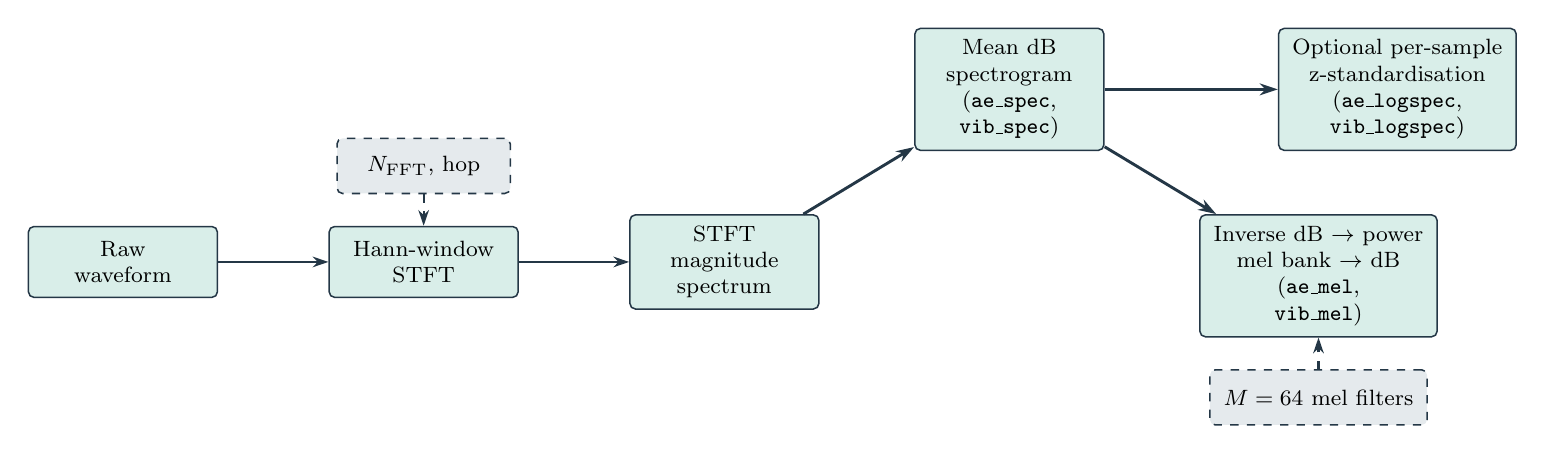
\begin{tikzpicture}[
  node distance=1.2cm and 1.4cm,
  box/.style={pub/representation, minimum width=2.4cm, minimum height=0.9cm},
  param/.style={pub/base, dashed, fill=pubSlateFill, minimum width=2.2cm, minimum height=0.7cm},
  arrow/.style={pub/arrow},
  splitarrow/.style={pub/flow}
]
\node[box] (raw) {Raw\\waveform};
\node[box, right=of raw] (stft) {Hann-window\\STFT};
\node[box, right=of stft] (lin) {STFT\\magnitude\\spectrum};
\node[box, above right=0.8cm and 1.2cm of lin] (db) {Mean dB\\spectrogram\\(\texttt{ae\_spec},\\\texttt{vib\_spec})};
\node[box, right=2.2cm of db] (z) {Optional per-sample\\z-standardisation\\(\texttt{ae\_logspec},\\\texttt{vib\_logspec})};
\node[box, below right=0.8cm and 1.2cm of db] (mel) {Inverse dB $\rightarrow$ power\\mel bank $\rightarrow$ dB\\(\texttt{ae\_mel},\\\texttt{vib\_mel})};
\node[param, above=0.4cm of stft] (stftp) {$N_{\rm FFT}$, hop};
\node[param, below=0.4cm of mel] (melp) {$M=64$ mel filters};
\draw[arrow] (raw) -- (stft);
\draw[arrow] (stft) -- (lin);
\draw[splitarrow] (lin) -- (db);
\draw[splitarrow] (db) -- (z);
\draw[splitarrow] (db) -- (mel);
\draw[arrow, dashed] (stftp) -- (stft);
\draw[arrow, dashed] (melp) -- (mel);
\end{tikzpicture}%
}
\caption{Preprocessing pipeline for AE and vibration signals. Raw
waveforms are transformed by a Hann-window STFT. The magnitude branch is
converted to dB and averaged over local maps; an optional per-sample
z-standardisation creates the historical \texttt{*\_logspec} caches. The
implemented log-mel branch inverse-converts the pass-mean dB cache to power,
applies the mel filter bank, and converts the result back to dB. All
representations are cached before model training. Because local maps are
averaged in dB before inverse conversion, this branch mel-filters a
geometric-mean power quantity rather than the arithmetic mean of local power
or log-mel maps.}
\label{fig:preprocessing-pipeline}
\end{figure}

\subsubsection{Time--frequency representations}

Short-time Fourier transforms are computed with a Hann window. For the
AE channel, the fast Fourier transform length is $N_{\text{FFT}}^{\rm
AE}=598$ samples and the hop length is $H^{\rm AE}=426$ samples,
yielding 300 frequency bins and 47 time frames per local AE map. For vibration,
$N_{\text{FFT}}^{\rm vib}=512$ and $H^{\rm vib}=426$, yielding 257
frequency bins and 13 time frames per local vibration map. The STFT complex coefficients are converted to magnitude and then to a decibel scale (clipped at $-80$~dB), producing local dB spectrogram maps. The AE cache has two planes labelled ``narrowband'' and ``broadband'' in the archived intermediate files; the available cache-generation code does not preserve the analogue/digital filter provenance needed to calibrate the channels' transfer paths. Raw-file metadata identify plane~1 as physical narrowband AE and plane~2 as physical broadband AE; this establishes channel provenance but not filter calibration. Both planes are included in every AE-dB and AE-dB-z configuration. The vibration arrays retain the three accelerometer axes. The effective frequency resolutions are
approximately $6.69$~kHz/bin for AE and
$100$~Hz/bin for vibration. Because the sampling rates differ by two
orders of magnitude, the stated STFT parameters yield different
effective physical window durations (transform lengths): approximately 150~\(\upmu\)s for AE and
10~ms for vibration, corresponding to total segment durations of approximately 5~ms and 
110~ms, respectively. The cached per-pass descriptor is not a single
middle-pass window. The per-pass intermediate \texttt{*\_spec.npz} files
contain \(N_p=2{,}910\) local maps for each modality and pass; the final
dataset-level \texttt{mean\_specs.npz} cache stores only their arithmetic
pass means with shapes \((319,2,300,47)\) and \((319,3,257,13)\). The retained intermediate cache does not
record the upstream local-map hop, overlap, terminal-window policy, or an
AE--vibration timestamp correspondence; consequently, ``aligned'' is not
claimed at event level. If the reported approximately 14.6~s pass duration
and uniform placement are assumed, 2,910 maps imply a nominal index spacing
of about 5.0~ms. This would imply negligible overlap for a 5~ms AE segment
and approximately 95\% overlap for a 110~ms vibration segment, but these are
arithmetic implications rather than recovered acquisition settings. The
common map index supports corresponding pass-position thirds only. For each pass \(p\), channel \(c\), frequency bin
\(f\), and STFT time frame \(t\), \texttt{compute\_mean\_spectrogram()}
stores
\begin{equation}
\bar S_{p,c,f,t}=\frac{1}{N_p}\sum_{j=1}^{N_p}S_{p,j,c,f,t}.
\label{eq:local-map-mean}
\end{equation}
This is a simple arithmetic mean over the local-map axis, with no temporal
weighting, selection, or learned aggregation. Thus the reported models use
a pass-level mean of local 5~ms AE and 110~ms vibration descriptors. This
averaging suppresses temporal ordering and transient localisation. A
retrospective early/middle/late-third and ordered three-window-concatenation
sensitivity analysis is reported in Supplementary
Table~\ref{tab:supp-pass-position}; fixed-distance windows and streaming
dispersion features remain future extensions. Both representations come
from the same grinding pass, but the fused inputs concatenate pass-level
descriptors with unequal local time extents. They are therefore not an
event-synchronised fusion. For tabular models, the maps are flattened and
concatenated, producing 38,223 features for fused full-resolution dB or dB-z
(\(2\times300\times47 + 3\times257\times13\)) and 8,512 features for fused
64-bin log-mel (\(2\times64\times47 + 3\times64\times13\)). Dimensions of the main
time--frequency representations are summarised in
Table~\ref{tbl:representation-dims}.

\begin{table}[htbp]
\centering
\caption{Dimensions of the principal time--frequency representations.
$N_{\rm FFT}$ is the transform length, $H$ the hop length, $C$ the number
of retained input planes or axes, $F$ the number of frequency bins, and
$T$ the number of time frames. For AE, $C=2$ denotes the physical narrowband and broadband AE channels; analogue filter specifications and gains are unavailable; for vibration, $C=3$ denotes the three accelerometer axes. The \texttt{*\_logspec} caches are per-sample z-standardised versions of the full-resolution dB maps, whereas the \texttt{*\_mel} caches are 64-bin log-mel maps.}
\label{tbl:representation-dims}
\begin{tabular}{@{}lccccc@{}}
\toprule
Representation & $N_{\rm FFT}$ & $H$ & $C$ & $F$ & $T$ \\
\midrule
\texttt{ae\_spec} & 598 & 426 & 2 & 300 & 47 \\
\texttt{vib\_spec} & 512 & 426 & 3 & 257 & 13 \\
\texttt{ae\_logspec} & 598 & 426 & 2 & 300 & 47 \\
\texttt{vib\_logspec} & 512 & 426 & 3 & 257 & 13 \\
\texttt{ae\_mel} & -- & -- & 2 & 64 & 47 \\
\texttt{vib\_mel} & -- & -- & 3 & 64 & 13 \\
\bottomrule
\end{tabular}
\end{table}

The historical \texttt{ae\_logspec} and \texttt{vib\_logspec} names denote
full-resolution dB spectrograms after per-sample, per-plane z-standardisation;
they do not apply an additional logarithm. They retain the 300 AE and
257 vibration frequency bins shown in Table~\ref{tbl:representation-dims}
and are standardised per sample and per channel. No subsequent fold-wise
spectral scaler is used in the RF experiments reported here. The 64-bin
log-mel descriptors are stored separately as \texttt{ae\_mel} and
\texttt{vib\_mel}. They are generated from the pass-mean dB cache by inverse
conversion to linear power, followed by multiplication by $M=64$ mel-spaced
filters covering the full Nyquist band. If $D$ is the pass-mean dB cache, the
implemented output is $10\log_{10}[\varepsilon + M(10^{D/10})]$ with a fixed global floor
$\varepsilon = 10^{-10}$ to avoid numerical underflow.
Because \(D\) is averaged over local maps in dB before this inverse
conversion, \(10^{D/10}\) is a geometric-mean power quantity. The implemented
cache is therefore distinct from an arithmetic pass-average of local
power-mel or log-mel maps; mel filtering and local-map averaging are not
interchangeable operations. Although originally
developed for audio, the mel-style filter bank is used here as a
logarithmic frequency-compression scheme rather than as a psychoacoustic
model. The mel-scale maps frequency $f$ (Hz) to
\begin{equation}
m = 2595 \log_{10}\!\left(1 + \frac{f}{700}\right),
\label{eq:mel}
\end{equation}
For the AE channel, the spectral representations cover the full Nyquist
band for empirical discrimination, but components above 1~MHz lie outside
the historically reported nominal AE response band and are interpreted
cautiously.
The full-resolution dB and 64-bin log-mel representations differ in both
frequency binning and amplitude transform. The dB-z caches differ from the
dB caches only by per-sample, per-plane z-standardisation. The canonical and
current RF spectral pipelines do not apply an additional fold-wise scaler to
spectrogram bins; therefore, the comparison is not a pure test of
mel-scale compression. The log-mel
variants (\texttt{ae\_mel}, \texttt{vib\_mel}) do not receive
per-sample normalisation; they therefore offer a partial sensitivity check
on whether removing absolute-energy information alters predictive
performance. A strict ablation omitting only per-sample/channel standardisation
is reported in Supplementary
Table~\ref{tab:supp-psnorm-ablation} and gives a small numerical mean-MAE
increase from 0.0210 to 0.0213~\(\upmu\)m without per-sample
standardisation. The maximum condition MAE increases from 0.1478 to
0.1863~\(\upmu\)m (Condition~7), so the ablation supports
mean-level robustness but not tail robustness.

Exact cache definitions, shapes, and SHA-256 provenance checksums are listed in Supplementary Table~\ref{tab:supp-cache-provenance}.
The available provenance for the two physical AE columns is separated from
the unavailable transfer-function information in Supplementary
Table~\ref{tab:supp-ae-plane-provenance}.

\subsubsection{Wavelet scattering and hand-crafted features}

Two-dimensional wavelet scattering transforms
(\texttt{ae\_wst}, \texttt{vib\_wst}) are computed with
\texttt{kymatio} \cite{mallat2012group}. We use second-order scattering
(\texttt{max\_order=2}) with $J=3$ octaves, Morlet wavelets, and
$L=8$ angular orientations (the constructor is
\texttt{Scattering2D(J=3, shape=(H,W), L=8, max\_order=2)}). Scattering coefficients are averaged over the
spatial (frequency--time) dimensions, producing a compact,
translation-invariant descriptor for each channel. The computation is
shown schematically in Figure~2. Note that for the vibration channel, the temporal dimension of the spectrogram is small ($T=13$ time frames). Using $J=3$ octaves corresponds to a maximum spatial support of $2^J = 8$ frames, which is close to the total signal length. Consequently, the wavelet filters at the largest scale ($j=2$) suffer from significant edge/boundary effects, and spatial averaging over this scale acts as a global smoother that discards almost all localized temporal variation, retaining only static spectral structures.

\begin{figure}[htbp]
\centering
\resizebox{\linewidth}{!}{%
\begin{tikzpicture}[
  node distance=1.4cm,
  box/.style={pub/representation, minimum width=2.6cm, minimum height=0.9cm},
  arrow/.style={pub/arrow}
]
\node[box] (spec) {2D spectrogram\\input};
\node[box, right=of spec] (psi1) {Morlet wavelet\\filter bank\\$L=8, J=3$};
\node[box, right=of psi1] (mod1) {Modulus\\$|\\cdot|$};
\node[box, right=of mod1] (psi2) {Second-order\\Morlet filters};
\node[box, right=of psi2] (mod2) {Modulus\\$|\\cdot|$};
\node[box, below=1.0cm of mod2] (avg) {Spatial\\averaging};
\node[box, left=of avg] (out) {Scattering\\coefficients};
\draw[arrow] (spec) -- (psi1);
\draw[arrow] (psi1) -- (mod1);
\draw[arrow] (mod1) -- (psi2);
\draw[arrow] (psi2) -- (mod2);
\draw[arrow] (mod2) -- (avg);
\draw[arrow] (avg) -- (out);
\end{tikzpicture}%
}
\caption{Wavelet scattering transform pipeline. A 2D spectrogram is
passed through two Morlet filter banks separated by modulus
nonlinearities, then spatially averaged to produce a compact,
translation-invariant descriptor per grinding pass.}
\label{fig:wst-pipeline}
\end{figure}

Time-domain statistics (\texttt{ae\_features}, \texttt{vib\_features})
include mean, standard deviation, skewness, kurtosis, RMS, peak, crest
factor, and frequency-domain band energy. Process parameters
(\texttt{pp}) are $v_s$, $v_w$, $a_p$. Physics-informed features
(\texttt{physics}) are heuristic indicators derived from process
parameters and sensor envelopes rather than dimensionally exact physical
quantities: AE wavelet energy (narrow 50--400\,kHz and broad 150--2000\,kHz
bands; the upper limit is capped at the AE Nyquist frequency of 2\,MHz,
and for the \texttt{cmor3-3} scales used the effective maximum frequency
is approximately 1.33\,MHz), AE burst rate (for each pass and band, $\sigma$ is computed from the
pass-level AE envelope after bandpass filtering; burst rate is the count
of envelope peaks above $4\sigma$, separated by at least 0.1\,ms. Because
$\sigma$ is computed per pass, the threshold is self-normalised and burst
rate captures relative burstiness rather than absolute AE amplitude), an equivalent chip-thickness proxy ($ec$), a normalized depth-of-cut
indicator ($bid=a_p/30$), a temperature-proxy term ($st$), envelope kurtosis for
the X/Y/Z vibration axes, and an overall vibration magnitude ($mag$). Each
indicator is aggregated over time by mean, standard deviation, maximum,
and minimum, producing a nominal 44-dimensional vector. A fold-wise audit
finds five globally constant aggregate columns (the two burst-rate minima
and the standard-deviation aggregates of (ec), (bid), and (st));
thus 39 columns vary across the campaign. These zero-variance columns are
retained for reproducibility, but fold-wise standardisation maps them to
zero and they must not be interpreted as independent physical
measurements. The audit is reported in Supplementary
Table~\ref{tab:supp-physics-audit}. The implemented process-derived and
temperature-indicator algorithms are specified directly in Supplementary
Table~\ref{tab:physics_features} and Equations~\eqref{eq:ec-implemented}--\eqref{eq:st-implemented}.
The archive does not preserve all filter settings for the burst features,
so those cached intermediate-derived values can be reused but are not
claimed to be fully reconstructible from raw signals. Because the
archived notes report the nominal AE response only up to 1~MHz, the 1--2\,MHz portion of
the broad band is retained only as an empirical descriptor and is not
interpreted as calibrated AE energy.

Tabular feature vectors and process parameters are standardised per fold
using training-set statistics. Spectrogram caches are not fold-wise scaled
in the canonical RF and current RF sensitivity pipelines. The dB-z cache is
instead normalised per sample and per channel before fitting; this removes
absolute energy information that may be physically meaningful. A strict
ablation that keeps the same RF architecture and omits only this per-sample
normalisation gives an overall LOGO
MAE of 0.0213~\(\upmu\)m, compared with 0.0210~\(\upmu\)m with
per-sample normalisation (Supplementary Table~\ref{tab:supp-psnorm-ablation}).
The result therefore does not
appear to depend on per-sample energy removal for mean LOGO MAE;
frequency-shape information appears sufficient for mean LOGO MAE in
this RF/dB-z configuration, although tail performance changes. Multimodal
tabular inputs are concatenated; multimodal deep-learning inputs are fed
through separate encoder branches that are fused before the regression
head.

\begin{figure}
\centering
\includegraphics[width=1\linewidth,height=\textheight,keepaspectratio]{methods_signal_representations.png}
\caption{Example signal representations for condition 10, sample 1
($R_a = 0.098~\upmu$m). (a)~AE dB spectrogram, (b)~AE log-mel
spectrogram, (c)~vibration (Z-axis) dB spectrogram, and
(d)~vibration log-mel spectrogram. The examples show dominant lower-frequency
energy in both modalities. Vibration below 5~kHz is compatible with structural
dynamics, whereas AE is treated as an empirical contact-related descriptor
because its transfer function is unavailable. Higher-frequency AE energy above 0.5~MHz and vibration energy near
17~kHz are located in frequency ranges commonly associated with
grain-contact and chatter-related dynamics, respectively.}
\label{fig:representations}
\end{figure}

\subsection{Predictive models}\label{predictive-models}

The model families share the outer LOGO test folds and metrics, with
model-specific training, validation, and preprocessing procedures
(Figure~\ref{fig:taxonomy}).

\textbf{Auditable classical baselines.} Ridge coefficients can be inspected
directly; the tree ensembles are analysed with post-hoc attribution. This is relevant to monitoring
workflows where model updates may be required after changes in wheel
grade, workpiece material, or dressing condition, although this workflow
is not tested here.

\begin{itemize}
\tightlist
\item
  \textbf{Ridge regression:} L2-regularised linear regression with
  $\alpha=1.0$; coefficients provide a signed importance score for every
  frequency bin.
\item
  \textbf{Random forest:} 200 trees, maximum depth 8, minimum 1 sample
  per leaf, $n_{\text{jobs}}=1$.
\item
  \textbf{LightGBM and XGBoost:} gradient-boosted trees with 200
  estimators, maximum depth 5, learning rate $0.05$, subsample
  $0.8$, and column sampling $0.8$.
\item
  \textbf{Shallow MLP:} two hidden layers of 128 and 64 units, L2
  penalty $\alpha=10^{-4}$, Adam optimiser with learning rate
  $10^{-3}$, early stopping on 10\% validation data, maximum 500
  iterations.
\end{itemize}

\textbf{Deep-learning baselines.} These models represent recent
literature on grinding monitoring:

\begin{itemize}
\tightlist
\item
  ResNet-style encoders for AE and vibration spectrograms
  (ResNetAECNN, ResNetVibCNN).
\item
  ResNet-based multimodal fusion (ResNetFusion).
\item
  Bilinear attention-based fusion network (BilinearFusionNetwork).
\item
  Multi-resolution spectrogram CNN.
\item
  Trajectory-based sequence CNN (TrajectoryCNN).
\item
  Graph-neural-network fusion (GraphNeuralNetworkFusion), TabTransformer (TabTransformerRegressor), and attention-based
  regressors.
\end{itemize}

Specifically, the advanced deep-learning baselines are structured as follows:
\begin{itemize}
\item \textbf{BilinearFusionNetwork:} uses dual ResNet encoders to extract feature maps from AE and vibration spectrograms, then applies low-rank bilinear pooling to fuse these representations with process parameters and physics-informed indicators before MLP regression.
\item \textbf{TrajectoryCNN:} is a sequence-based model that utilizes 1D temporal convolutions to process temporal sub-band energy trajectories from AE and vibration, capturing localized time-dependent dynamics instead of relying on time-averaged summaries.
\item \textbf{GraphNeuralNetworkFusion:} frames multimodal fusion as a graph learning task where individual modalities (AE, vibration, physics, parameters) represent nodes in a fully-connected graph. Node features are processed via Graph Attention Network (GAT) layers for cross-modal message passing, followed by global average graph pooling.
\item \textbf{TabTransformerRegressor:} embeds continuous features (physics, process parameters) by scaling a learned feature-specific embedding vector by the continuous scalar value and adding a bias. These embedded feature sequences are then processed by a multi-layer Transformer encoder.
\end{itemize}

The best-performing spectrogram CNN, ResNetVibCNN, processes vibration
dB spectrograms of shape $(3, 257, 13)$ through a stem convolution,
two residual blocks with squeeze-and-excitation attention and dropout
$p=0.3$, global average pooling, and a fully connected regressor with a
64-dimensional hidden layer. Its architecture is shown in
Figure~4. All deep-learning models are trained
with AdamW (learning rate $10^{-3}$, weight decay $10^{-4}$), MSE loss,
a ReduceLROnPlateau scheduler (factor $0.5$, patience 5 epochs), early
stopping (patience 20 epochs), and a maximum of 200 epochs. Batch sizes
are 16 for the ResNet encoders and 32 otherwise. The historical planned
comparison uses the canonical seed-42 results for all model--configuration
pairs; reproducible current RF reruns are reported before those artifacts in
the Results. To quantify training stochasticity, a secondary equal-budget
sensitivity analysis repeats the main stochastic architectures over five
seeds; details are provided in Section~\ref{experimental-workflow}.

\begin{figure}[htbp]
\centering
\resizebox{0.98\linewidth}{!}{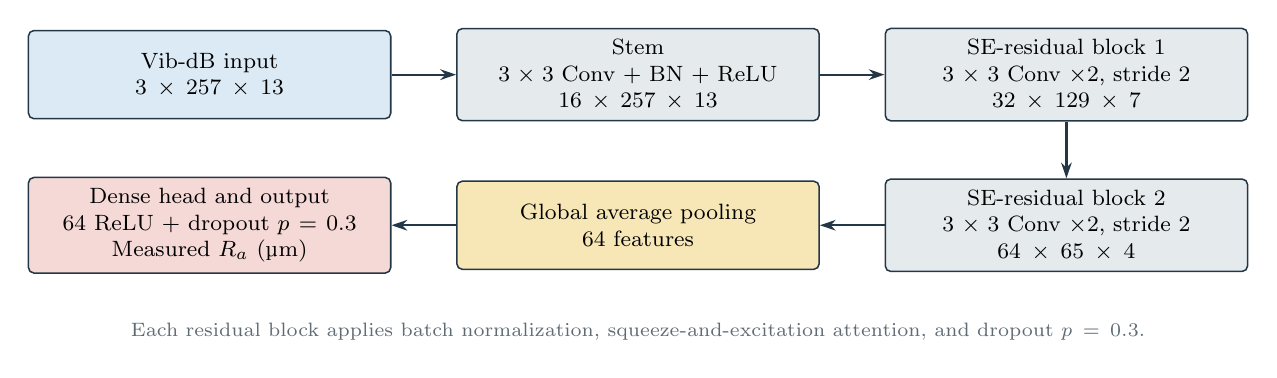
\begin{tikzpicture}[
    node distance=0.72cm and 0.82cm,
    stage/.style={pub/model, text width=4.25cm, minimum height=1.12cm},
    arrow/.style={pub/arrow},
]
\node[pub/input, text width=4.25cm, minimum height=1.12cm] (input)
  {Vib-dB input\\$3\times257\times13$};
\node[stage, right=of input] (stem)
  {Stem\\$3\times3$ Conv + BN + ReLU\\$16\times257\times13$};
\node[stage, right=of stem] (res1)
  {SE-residual block 1\\$3\times3$ Conv $\times2$, stride 2\\$32\times129\times7$};

\node[stage, below=of res1] (res2)
  {SE-residual block 2\\$3\times3$ Conv $\times2$, stride 2\\$64\times65\times4$};
\node[pub/explanation, text width=4.25cm, minimum height=1.12cm, left=of res2] (gap)
  {Global average pooling\\$64$ features};
\node[pub/target, text width=4.25cm, minimum height=1.12cm, left=of gap] (head)
  {Dense head and output\\$64$ ReLU + dropout $p=0.3$\\Measured $R_a$ (\textmu m)};

\draw[arrow] (input) -- (stem);
\draw[arrow] (stem) -- (res1);
\draw[arrow] (res1) -- (res2);
\draw[arrow] (res2) -- (gap);
\draw[arrow] (gap) -- (head);
\node[pub/note, text width=13.6cm, align=center, below=0.55cm of gap]
  {Each residual block applies batch normalization, squeeze-and-excitation attention, and dropout $p=0.3$.};
\end{tikzpicture}%
}
\caption{ResNetVibCNN architecture for vibration dB spectrogram
regression. The three-axis input is processed by a stem convolution and
two stride-two SE-residual blocks. Each residual block contains batch
normalisation, squeeze-and-excitation attention, and dropout; global average
pooling and a 64-unit dense head produce the measured-$R_a$ estimate.}
\label{fig:resnetvibcnn-arch}
\end{figure}

Table~\ref{tbl:dl-baselines} summarises the deep-learning baselines and
their input configurations.

\begin{table}[htbp]
\centering
\caption{Overview of the deep-learning baselines. The column ``Input''
uses the abbreviations defined in Table~\ref{tbl:config-abbreviations}.}
\label{tbl:dl-baselines}
\begin{tabular}{@{}llll@{}}
\toprule
Model & Input & Key mechanism & Fusion \\
\midrule
ResNetAECNN & AE-dB & ResNet encoder + SE & Single modality \\
ResNetVibCNN & Vib-dB & ResNet encoder + SE & Single modality \\
ResNetFusion & AE-dB + Vib-dB & Dual ResNet encoders & Early fusion \\
BilinearFusion & AE-dB + Vib-dB + phys + PP & Bilinear attention & Late fusion \\
Multi-resolution CNN & Vib-dB & Multi-scale convolutions & Single modality \\
Trajectory CNN & \texttt{Vib-traj} & 1D sequence CNN on temporal sub-bands & Single modality \\
GNN fusion & AE-dB + Vib-dB & Graph neural network & Structured fusion \\
TabTransformer & \texttt{AE/Vib feats + phys + PP} & Transformer on tabular & Tabular multimodal \\
Attention regressor & AE-dB + Vib-dB & Self-attention & Late fusion \\
\bottomrule
\end{tabular}
\end{table}

\begin{figure}
\centering
\resizebox{0.98\linewidth}{!}{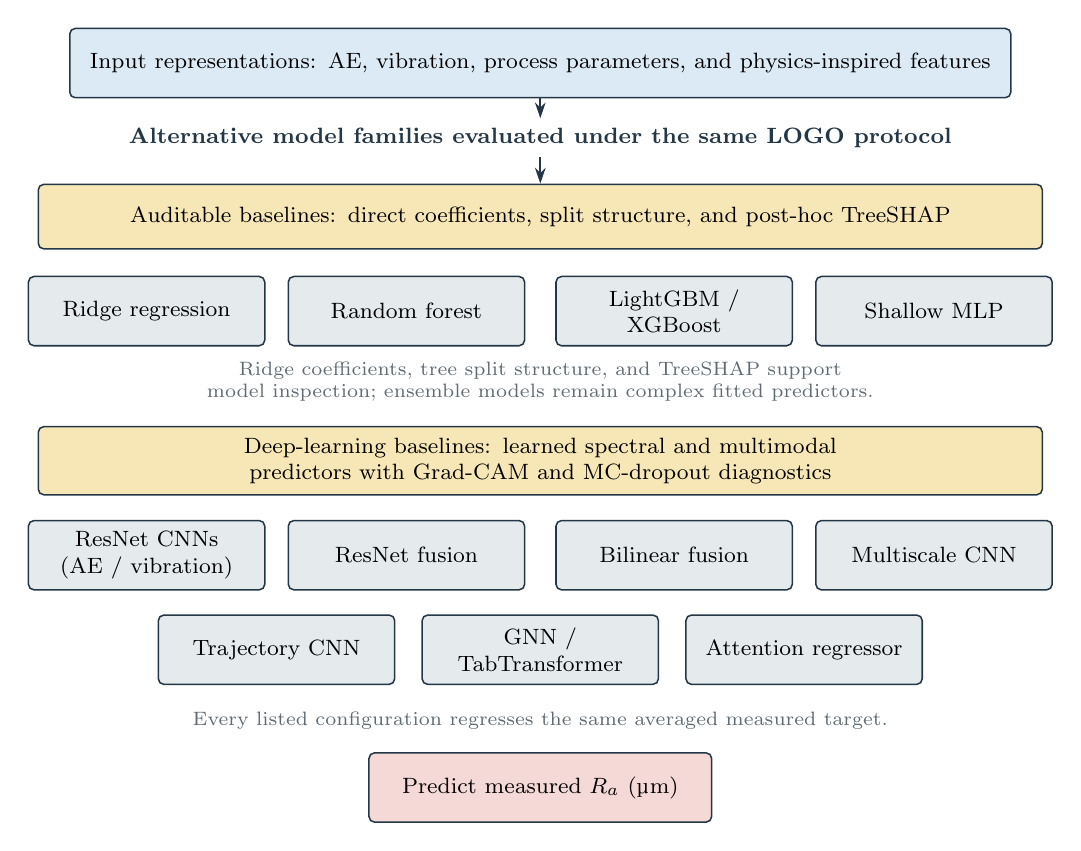
\begin{tikzpicture}[
    arrow/.style={pub/arrow},
    family/.style={pub/explanation, text width=12.4cm, minimum height=0.82cm},
    modelcard/.style={pub/model, text width=2.65cm, minimum height=0.88cm},
]
\node[pub/input, text width=11.6cm, minimum height=0.88cm] (input) at (0,6.4)
  {Input representations: AE, vibration, process parameters, and physics-inspired features};
\node[pub/heading] (choice) at (0,5.45)
  {Alternative model families evaluated under the same LOGO protocol};
\draw[arrow] (input) -- (choice);

\node[family] (auditable) at (0,4.45)
  {Auditable baselines: direct coefficients, split structure, and post-hoc TreeSHAP};
\draw[arrow] (choice) -- (auditable);
\node[modelcard] (ridge) at (-5.0,3.25) {Ridge regression};
\node[modelcard] (rf) at (-1.7,3.25) {Random forest};
\node[modelcard] (lgbm) at (1.7,3.25) {LightGBM /\\XGBoost};
\node[modelcard] (mlp) at (5.0,3.25) {Shallow MLP};
\node[pub/note, text width=12.0cm, align=center] at (0,2.35)
  {Ridge coefficients, tree split structure, and TreeSHAP support model inspection; ensemble models remain complex fitted predictors.};

\node[family] (deep) at (0,1.35)
  {Deep-learning baselines: learned spectral and multimodal predictors with Grad-CAM and MC-dropout diagnostics};
\node[modelcard] at (-5.0,0.15) {ResNet CNNs\\(AE / vibration)};
\node[modelcard] at (-1.7,0.15) {ResNet fusion};
\node[modelcard] at (1.7,0.15) {Bilinear fusion};
\node[modelcard] at (5.0,0.15) {Multiscale CNN};
\node[modelcard] at (-3.35,-1.05) {Trajectory CNN};
\node[modelcard] at (0,-1.05) {GNN /\\TabTransformer};
\node[modelcard] at (3.35,-1.05) {Attention regressor};

\node[pub/note, text width=12.0cm, align=center] at (0,-1.95)
  {Every listed configuration regresses the same averaged measured target.};
\node[pub/target, text width=4.0cm, minimum height=0.88cm] at (0,-2.8)
  {Predict measured $R_a$ (\textmu m)};
\end{tikzpicture}%
}
\caption{Model taxonomy evaluated in this study. The left branch contains
a directly inspectable regularised linear model and auditable tree ensembles
supported by post-hoc SHAP values. The right branch uses deep-learning
baselines whose decisions are analysed post-hoc with Grad-CAM and
MC-dropout. Both branches predict $R_a$ and are compared under the same
LOGO protocol.}
\label{fig:taxonomy}
\end{figure}

\begin{table}[htbp]
\centering
\caption{Key hyperparameters of the main auditable classical and baseline models.
Fixed hyperparameters were applied uniformly across all LOGO folds; deep-learning
entries (Shallow MLP) used additional early-stopping on the validation fold.}
\label{tbl:hyperparams}
\setlength{\tabcolsep}{8pt}
\renewcommand{\arraystretch}{1.25}
\begin{tabular}{@{}llr@{}}
\toprule
\textbf{Model} & \textbf{Hyperparameter} & \textbf{Value} \\
\midrule
Ridge                & Regularisation strength $\alpha$   & 1.0 \\
\addlinespace[4pt]
Random forest        & Number of trees                    & 200 \\
                     & Max depth                          & 8 \\
                     & Min samples per leaf               & 1 \\
\addlinespace[4pt]
LightGBM             & Number of estimators               & 200 \\
                     & Max tree depth                     & 5 \\
                     & Learning rate                      & 0.05 \\
                     & Subsample ratio                    & 0.8 \\
\addlinespace[4pt]
XGBoost              & Number of estimators               & 200 \\
                     & Max tree depth                     & 5 \\
                     & Learning rate                      & 0.05 \\
                     & Subsample ratio                    & 0.8 \\
\addlinespace[4pt]
Shallow MLP          & Hidden layers                      & (128, 64) \\
                     & L2 regularisation $\alpha$         & $10^{-4}$ \\
                     & Learning rate                      & $10^{-3}$ \\
\bottomrule
\end{tabular}
\end{table}

\subsection{Validation protocol}\label{validation-protocol}

We use strict leave-one-condition-out (LOGO) cross-validation with 16
outer folds. In each fold, one condition is held out as the test set, a
second condition is reserved for early-stopping validation, and the
remaining 14 conditions are used for training
(Figure~\ref{fig:logo}). The validation condition is selected from the
remaining conditions by successive draws from
\texttt{numpy.random.RandomState(42)} in ascending test-condition order.
The resulting train/validation/test split is
therefore identical for every model evaluated on a given fold. This prevents
information leakage across samples that share the same grinding
condition and measures whether a model generalises to previously unseen
process states. Typical fold sizes are approximately 280 training,
20 validation, and 20 test samples. The deterministic fold assignment is
shown in Figure~\ref{fig:logo-matrix}. Because only one validation
condition is used per fold, the validation loss is potentially volatile and
sensitive to that condition's characteristics. A fixed-hyperparameter
rotation diagnostic is reported for ResNetVibCNN and ResNetAECNN in
Supplementary Table~\ref{tab:supp-deep-validation-rotation}: it compares
the canonical seed-42 validation draw with a cyclic-next-condition
validation assignment. It tests early-stopping sensitivity only; it does
not rerun the original hyperparameter search or provide inner grouped model
selection. Tabular models such as RF use fixed hyperparameters and do not
rely on this early-stopping signal.
The exact 16 assignments are listed in Supplementary
Table~\ref{tab:supp-logo-assignments}; Figure~\ref{fig:logo-matrix} is
generated from the same rule and archived assignment CSV.

A model-selection caveat applies. The deep-learning entries were tuned
by random search over model and training hyperparameters (with a hyperparameter search space size of approximately 20 configurations per architecture) using the same
outer LOGO folds (the validation fold was used for early stopping and the
test fold was used for final model selection). The tree-based models used
fixed hyperparameters (Table~\ref{tbl:hyperparams}). This is not a fully
nested leave-one-condition-out comparison; using the held-out test fold
for final model selection means the deep-learning results are
post-selection estimates rather than unbiased generalisation estimates.
The reported differences should therefore be read as rankings under a
fixed evaluation budget rather than as population estimates of
generalisation error. This post-selection caveat applies to the selected
best RF as well as to the deep-learning entries. The primary purpose of
the benchmark is comparative evidence within this dataset, not an
unbiased population estimate.

The primary planned statistical testing is performed on the canonical seed-42 results using paired Wilcoxon signed-rank tests. However, because training sets overlap substantially across folds (each pair of training sets shares 13 out of 14 conditions), the fold MAEs are not strictly independent. This violation of the independence assumption means the resulting p-values must be interpreted as exploratory indicators of relative performance rather than strict, independent probability assessments. A secondary sensitivity analysis using five random seeds (42--46) is conducted to assess training stochasticity, as described in Section~\ref{experimental-workflow}.

\begin{figure}[htbp]
\centering
\includegraphics[width=89mm]{methods_logo_matrix.png}
\caption{Leave-one-condition-out fold assignment. Rows correspond to the
16 LOGO folds; columns correspond to the 16 grinding conditions. In each
fold the test condition is red, the validation condition is orange, and
the 14 training conditions are blue.}
\label{fig:logo-matrix}
\end{figure}

\begin{figure}
\centering
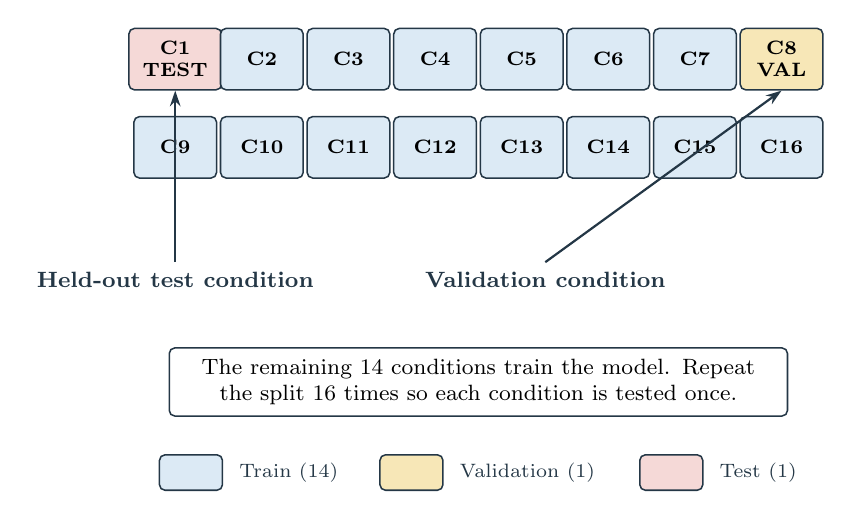
\begin{tikzpicture}[
    train/.style={pub/train},
    val/.style={pub/validation},
    test/.style={pub/test},
    arrow/.style={pub/arrow},
    ann/.style={pub/heading},
]

% One representative LOGO fold. The caption supplies the full figure title.
\foreach \c in {1,...,16} {
    \pgfmathsetmacro{\col}{mod(\c-1,8)}
    \pgfmathsetmacro{\row}{floor((\c-1)/8)}
    \pgfmathsetmacro{\x}{\col*1.10}
    \pgfmathsetmacro{\y}{0.45 - \row*1.12}
    \ifnum\c=1
        \node[test] (C\c) at (\x,\y) {C\c\\TEST};
    \else\ifnum\c=8
        \node[val] (C\c) at (\x,\y) {C\c\\VAL};
    \else
        \node[train] (C\c) at (\x,\y) {C\c};
    \fi\fi
}

\node[ann] (annTest) at (0.0,-2.35) {Held-out test condition};
\draw[arrow] (annTest.north) -- (C1.south);
\node[ann] (annVal) at (4.7,-2.35) {Validation condition};
\draw[arrow] (annVal.north) -- (C8.south);

\node[pub/base, fill=white, text width=7.5cm] at (3.85,-3.65) {
  The remaining 14 conditions train the model. Repeat the split 16 times so each condition is tested once.
};

\node[train, minimum width=0.8cm, minimum height=0.45cm] (legT) at (0.2,-4.8) {};
\node[right=0.08cm of legT, pub/legend] {Train (14)};
\node[val, minimum width=0.8cm, minimum height=0.45cm] (legV) at (3.0,-4.8) {};
\node[right=0.08cm of legV, pub/legend] {Validation (1)};
\node[test, minimum width=0.8cm, minimum height=0.45cm] (legTe) at (6.3,-4.8) {};
\node[right=0.08cm of legTe, pub/legend] {Test (1)};
\end{tikzpicture}%

\caption{Leave-one-condition-out cross-validation, illustrated with
canonical fold 1 (Condition 1 test; Condition 8 validation). Each of the 16
conditions is used once as the test fold (red); a different condition
serves as the validation fold (orange); the remaining 14 conditions are
used for training (blue). Per-fold performance is summarised by MAE, and
the 16 per-fold MAEs are aggregated as mean~$\pm$~std. Pairwise model
comparisons use the Wilcoxon signed-rank test with Holm-Bonferroni
correction.}
\label{fig:logo}
\end{figure}

The primary metric is mean absolute error (MAE) in micrometres:
\begin{equation}
\mathrm{MAE} = \frac{1}{N}\sum_{i=1}^{N} |y_i - \hat{y}_i|.
\label{eq:mae}
\end{equation}
We report mean~$\pm$~standard deviation of MAE across the 16 folds.
Bootstrap 95\% confidence intervals are computed with $B=1000$
replicates on the per-fold MAEs using the percentile method. Pairwise
comparisons use the two-sided Wilcoxon signed-rank test paired by LOGO
fold, with Holm-Bonferroni correction at family-wise error rate
$\alpha=0.05$. This statistical workflow is shown in
Figure~\ref{fig:statistical-workflow}.
The implementation uses \texttt{scipy.stats.wilcoxon} with
\texttt{zero\_method='zsplit'}; tied absolute differences receive average
ranks. Hodges--Lehmann intervals use 5,000 percentile bootstrap resamples
of the 16 paired fold differences with random seed 42. The point estimate
is the median of all Walsh averages $\{(d_i+d_j)/2:i\leq j\}$ of the
paired differences. These intervals are unadjusted descriptive intervals;
multiplicity correction applies only to the Wilcoxon $p$-values. Rank-biserial
correlation is the signed-rank sum divided by the total rank sum after
removing zero differences. No exact zero paired differences occur in the
reported 14 comparisons, so this removal does not create a discrepancy with
the Wilcoxon zero-handling rule.

\begin{figure}[htbp]
\centering
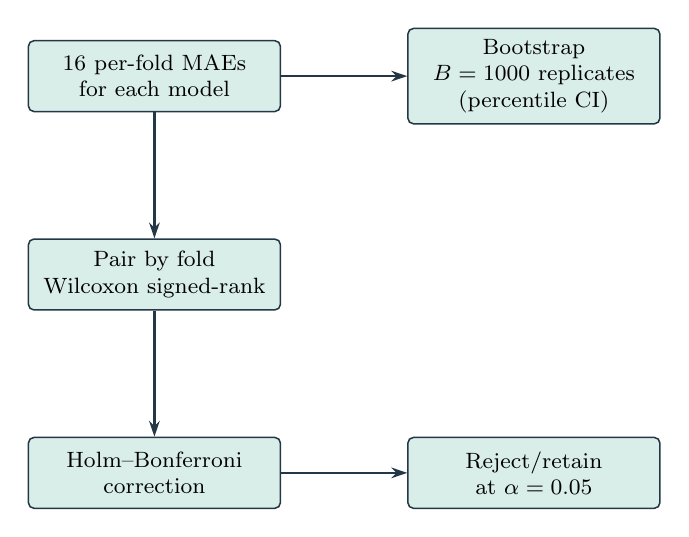
\begin{tikzpicture}[
  node distance=1.6cm,
  box/.style={pub/representation, minimum width=3.2cm, minimum height=0.9cm},
  arrow/.style={pub/arrow}
]
\node[box] (mae) {16 per-fold MAEs\\for each model};
\node[box, right=of mae] (boot) {Bootstrap\\$B=1000$ replicates\\(percentile CI)};
\node[box, below=of mae] (pair) {Pair by fold\\Wilcoxon signed-rank};
\node[box, below=of pair] (holm) {Holm--Bonferroni\\correction};
\node[box, right=of holm] (decide) {Reject/retain\\at $\alpha=0.05$};
\draw[arrow] (mae) -- (boot);
\draw[arrow] (mae) -- (pair);
\draw[arrow] (pair) -- (holm);
\draw[arrow] (holm) -- (decide);
\end{tikzpicture}
\caption{Statistical comparison workflow. Per-fold MAEs are used both to
build bootstrap confidence intervals and to perform paired Wilcoxon tests;
$p$-values are adjusted with Holm--Bonferroni correction.}
\label{fig:statistical-workflow}
\end{figure}

\subsection{Explainability and uncertainty}\label{explainability-and-uncertainty}

To assess whether the predictions can be audited, selected top models
are analysed using coefficient-, SHAP-, Grad-CAM-, and uncertainty-based
diagnostics.

\textbf{Model-attribution analyses.}
Ridge regression yields a signed coefficient for every frequency bin,
providing a global linear attribution; Figure~\ref{fig:xai-methods}a
shows the coefficient magnitudes for \texttt{vib\_spec}, which
concentrate in the low-frequency chatter and structural bands. TreeSHAP is applied to both (i)~the LightGBM model trained on
\texttt{ae\_spec+vib\_spec} as a representative tree-based model, and
(ii)~the recommended random forest trained on fused AE and vibration
dB-z descriptors (\texttt{AE-dB-z + Vib-dB-z}). For the
LightGBM model the training set is used as the background distribution
with exact TreeSHAP computations; for the random forest we use the
path-dependent TreeSHAP approximation. The LightGBM vibration profile
contains a sparse high-importance bin near 22~kHz. This lies in a
structural-frequency region, but neither a specific grinding mechanism nor
sensor/fixture resonance can be separated from the present data
(Figure~\ref{fig:xai-methods}b). The full ranked
SHAP importance for the LightGBM model is shown in Figure~\ref{fig:xai},
and the pooled out-of-fold SHAP profile for the current 14-condition RF/dB-z
pipeline is shown in Supplementary Figure~\ref{fig:supp-shap-rf}. It shows
AE importance above approximately
300~kHz and dominant vibration importance between approximately 16 and
24~kHz, with the largest pooled bin near 16.2~kHz. The profiles share a broad separation between
higher-frequency AE information and structural-frequency vibration
information, but their dominant bins differ by model and representation.
For each TreeSHAP analysis, feature importance is first defined as the mean
absolute SHAP value over the sampled explanatory passes. It is then averaged
over STFT time frames, retained separately by AE plane or vibration axis,
and summed within each reported physical-frequency band. Each modality and
explainer is normalised independently to 100\% only after this pooling.
The flattened arrays use NumPy C order. Within a modality, flattened feature
index $k=((cF)+f)T+t$ maps to channel/plane $c$, frequency bin $f$, and time
frame $t$; the vibration block begins after the $2\times300\times47$ AE
features. Physical frequency is $f f_s/N_{\rm FFT}$. This mapping is used by
both the plotted profiles and the archived per-frequency CSV files.
The attribution protocols are distinct. First, LightGBM uses a global
explanatory refit with 30 background and 50 explained passes as an
illustrative exact-tree explanation. Second, the RF analysis refits the
reproducible current 14-condition RF/dB-z pipeline in each LOGO fold and
explains only that fold's held-out condition using path-dependent TreeSHAP;
fold-specific profiles are pooled only after out-of-fold explanation. It
therefore explains the current RF predictions, not the historical canonical
0.0200~\(\upmu\)m artifact. Third, ResNetVibCNN uses Grad-CAM as described
below. No global RF explanation is used for the reported RF frequency profile.

For the deep-learning baseline ResNetVibCNN, Grad-CAM is computed on the
last convolutional layer to visualise the spectrogram regions that drive
predictions. The aggregated Grad-CAM frequency profile highlights chatter
and structural frequencies below 15~kHz, with additional high-frequency
vibration sensitivity above 15~kHz that may reflect wheel--spindle
structural response or high-frequency vibration modes. Because the input
is vibration, this high-frequency sensitivity should not be interpreted as
acoustic-emission energy (Figure~\ref{fig:xai-methods}c).
For Grad-CAM, the absolute activation map is averaged over all analysed
passes after bilinear interpolation from the final convolutional map to the
original \(257\times13\) vibration-STFT grid, then averaged over time frames
to produce the frequency profile. Thus CSV frequency bin \(k\) maps to
\(k\times 51{,}200/512\)~Hz. Interpolation supplies a common display grid;
the saliency still represents the receptive fields of the pooled
convolutional features rather than an isolated original-STFT bin.

\begin{figure}[htbp]
\centering
\includegraphics[width=\textwidth]{methods_xai_comparison.png}
\caption{Explainability methods applied to real grinding data. (a)~Ridge
regression coefficient magnitudes for Vib-dB. (b)~TreeSHAP
mean $|\text{SHAP}|$ for LightGBM on Vib-dB.
(c)~Grad-CAM frequency importance for ResNetVibCNN on Vib-dB.
Shaded bands mark low-frequency structural modes (green) and
higher-frequency vibration/chatter regions (blue).}
\label{fig:xai-methods}
\end{figure}

\textbf{Physics-consistency checks.}
Important bins are mapped to physical frequencies. For AE spectrograms
the bin spacing is approximately $6.69$~kHz/bin; for vibration
spectrograms it is approximately $100$~Hz/bin. A bin is considered
consistent with a known grinding mechanism if its centre frequency lies
within $\pm$10\% of an expected peak frequency for that mechanism; the
tolerance is intended only for narrow peak matching, whereas broad bands
such as 2--15~kHz are interpreted qualitatively. The band edges are
approximate and the tolerance is applied to the centre frequency rather
than to the band edges. In this study the expected bands are approximated
as: spindle rigid-body motion and low-order spindle drift below 500~Hz;
chatter and structural vibration roughly 2--15~kHz; and grain-contact
acoustic emission above 100~kHz, with the historically reported
100~kHz--1~MHz nominal band used only as a cautious reporting convention.
Figure~\ref{fig:bandmass} shows how the total attribution
mass is distributed across physical frequency bands for the three
explainers; the mass is concentrated in frequency regions that are
physically plausible for grinding dynamics.

\textbf{Uncertainty quantification.}
MC-dropout with 50 stochastic forward passes is used to quantify
predictive uncertainty for ResNetVibCNN on Vib-dB. All 16
uncertainty-analysis LOGO checkpoints are loaded without retraining,
substitution, or non-strict state-dictionary matching. Deterministic and
stochastic predictions are recomputed from each same checkpoint in one run.
These checkpoints give a deterministic mean fold MAE of 0.0443~\(\upmu\)m
and are not the distinct canonical 0.0268~\(\upmu\)m result artifact.
Dropout layers remain active at test time while
batch-normalisation layers are kept in evaluation mode so that small test
batches do not shift the population statistics. All dropout layers in the
network are activated for the stochastic passes, so the stochastic-forward
mean is treated as an uncertainty diagnostic and not as a recalibrated
deterministic predictor. The mean and variance of the 50 outputs form the
point prediction and the epistemic standard deviation, respectively. The
reported 95\% interval is computed as
\(\hat y \pm 1.96\,\sigma_{\text{MC}}\) and should be interpreted as an
illustrative epistemic interval rather than a calibrated predictive
interval including aleatoric uncertainty. The MC-dropout analysis is
evaluated under the same 16-fold LOGO protocol used for accuracy, so
every condition---including Condition~7---appears as a held-out test set
once. Figure~\ref{fig:uncertainty-methods} shows the resulting prediction
intervals sorted by predicted mean, a reliability diagram relating
predicted standard deviation to observed absolute error, and the
empirical coverage within each uncertainty bin. Across all 319 held-out
samples the aggregate coverage is 50.2\%, the mean interval width is
0.0479~\(\upmu\)m, the mean absolute error of the stochastic-mean prediction
is 0.0452~\(\upmu\)m, and the Pearson correlation between predicted standard
deviation and observed absolute error is 0.488. Although predicted
standard deviation is therefore correlated with absolute error, the
intervals remain far below the nominal 95\% level; MC-dropout does not
provide a calibrated predictive interval for this CNN. Condition~7 has
0\% coverage. A smaller 59-sample subset (Conditions 1, 2, and 6)
previously gave 100\% coverage but with a wider mean width
(0.073~\(\upmu\)m versus 0.0479~\(\upmu\)m under full LOGO), showing that the
apparent calibration of MC-dropout is highly sensitive to which conditions
are included.
Figure~\ref{fig:uncertainty-calibration} shows the per-sample
relationship between predicted standard deviation and observed absolute
error for the full LOGO evaluation.

For a separate 15-condition RF uncertainty variant, intervals are computed as
\(\hat y \pm c \, \sigma_{\text{tree}}\), where
\(\sigma_{\text{tree}}\) is the standard deviation of the individual
tree predictions. Within outer fold \(g\), let \(\bar y_i^{\rm OOB}\) and
\(s_i^{\rm OOB}\) be the mean and standard deviation over trees for which
training sample \(i\) is out of bag. The global factor is
\[
c_g=Q_{0.95}\left\{\frac{|y_i-\bar y_i^{\rm OOB}|}
{s_i^{\rm OOB}+10^{-8}}:i\in\mathcal T_g\right\},
\]
where \(Q_{0.95}\) is NumPy's default linear empirical quantile. The
condition-aware variant uses the same score restricted to samples from the
three Euclidean-nearest training conditions after min--max normalisation of
wheel speed, workpiece speed, and depth. The split variant removes the
single nearest condition from model fitting and applies the same scaled-score
quantile on that calibration condition. The naive variant uses
\(Q_{0.95}(|y_i-\bar y_i^{\rm OOB}|)\) directly, without tree-variance
scaling. Zero tree standard deviations are stabilised by \(10^{-8}\), and
all fitting, neighbour selection, and calibration are repeated independently
inside each outer fold. These are diagnostic post-hoc intervals, not formal
finite-sample conformal guarantees or intervals for the current 14-condition
benchmark RF.

\begin{figure}[htbp]
\centering
\includegraphics[width=\textwidth]{methods_uncertainty_overview.png}
\caption{Full 16-fold LOGO MC-dropout uncertainty for ResNetVibCNN on
Vib-dB. (a)~Nominal 95\% MC-dropout epistemic intervals and observed $R_a$
sorted by predicted mean. (b)~Reliability diagram: mean predicted
standard deviation versus mean observed absolute error per bin.
(c)~Empirical coverage per uncertainty bin against the nominal 95\%
level. Aggregate coverage is 50.2\% and mean interval width is
0.0479~\(\upmu\)m, indicating that MC-dropout is under-covering on this
CNN; the intervals are correlated with error but are not calibrated.}
\label{fig:uncertainty-methods}
\end{figure}

\subsection{Experimental workflow}\label{experimental-workflow}

The study follows a four-stage workflow: (1)~preprocessing of raw AE and
vibration signals and caching of all candidate representations; (2)~LOGO
training and evaluation of every model--configuration pair under the
same protocol; (3)~ranking, bootstrap confidence intervals, and
statistical testing; and (4)~post-hoc explainability and uncertainty
analysis of the top-performing systems. A high-level overview of the
pipeline is shown in Figure~\ref{fig:workflow}.

Because the 16 LOGO folds are deterministic and exhaustive over the
available grinding conditions, repeating the outer cross-validation would
not create new validation evidence. The historical planned comparison uses
the canonical seed-42 results and the pre-defined 14-comparison
Holm-corrected testing family.  To quantify training stochasticity, a
secondary sensitivity analysis trained the main stochastic architectures
(ResNetVibCNN, TrajectoryCNN, ResNetAECNN, ChannelAttentionCNN, ResNetFusion, BilinearFusionNetwork, and
the recommended random forest) under the same 16 outer LOGO folds with
five different random seeds. In every outer fold, the repeated RF excludes
the same canonical validation condition as the neural models and therefore
uses the same 14-condition training-data budget. The earlier 15-condition RF
repeat is retained only as a deployment-style sensitivity and is excluded
from the paired model-family tests. The reported seed-averaged MAE is the mean
over these five seeds; seed-level overall MAEs are given in
Supplementary Table~\ref{tab:supp-seed-level}.  For the sensitivity
analysis, per-condition MAEs were first averaged over seeds, preserving
the 16 condition-level paired observations; the 16 condition-level values
were not inflated by treating folds and seeds as independent samples.
This seed-repeat analysis provides a robustness check for training
stochasticity and is not treated as the primary inferential comparison.

The historical shallow-MLP baseline used scikit-learn's internal random
10\% validation fraction and is therefore an implementation-specific member
of the archived 14-comparison family. A corrected sensitivity uses the same
designated whole validation condition as the other models, standardises inputs
and targets from the 14-condition fitting subset only, disables the internal
random validation split, and selects among three training-only
architecture/regularisation settings. This corrected run is reported as a
separate sensitivity rather than substituted into the historical family.

\begin{figure}[htbp]
\centering
\resizebox{\linewidth}{!}{%
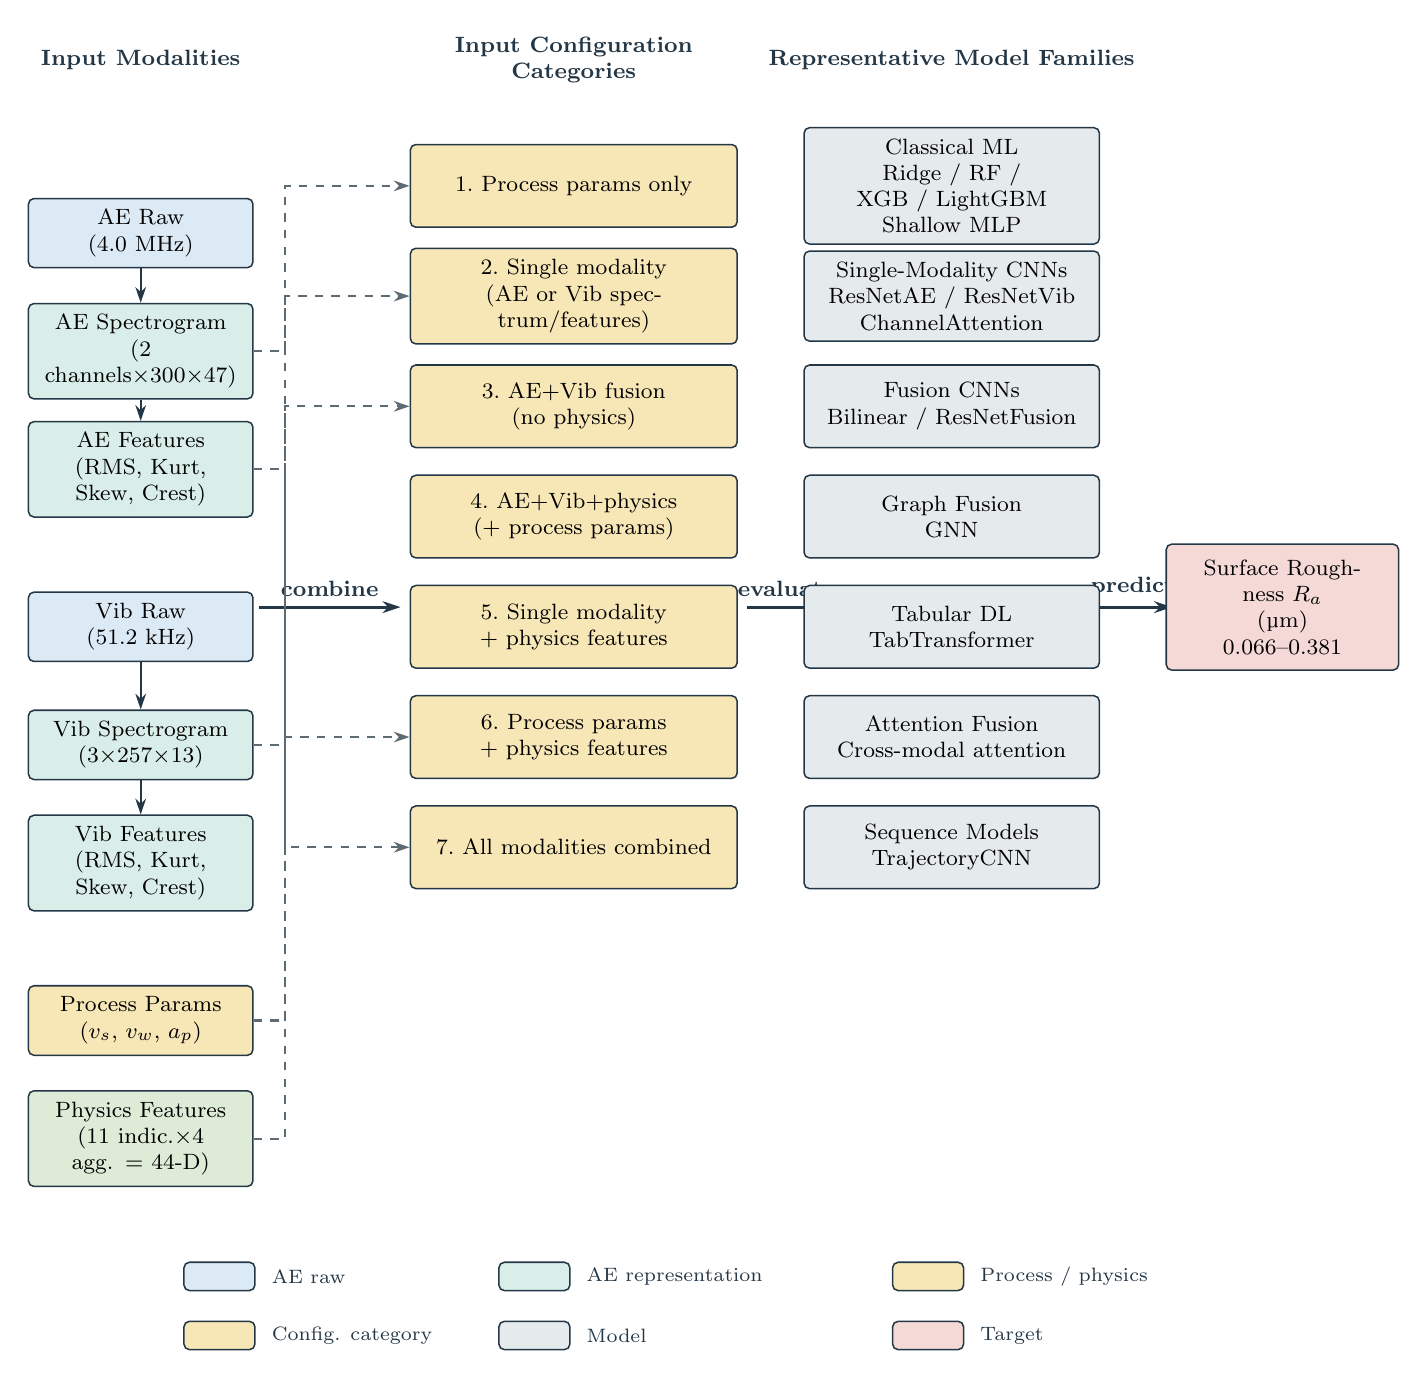
\begin{tikzpicture}[
    raw/.style={pub/input, minimum width=2.6cm, minimum height=0.85cm, text width=2.5cm},
    rep/.style={pub/representation, minimum width=2.6cm, minimum height=0.85cm, text width=2.5cm},
    pp/.style={pub/process, minimum width=2.6cm, minimum height=0.85cm, text width=2.5cm},
    phys/.style={pub/physics, minimum width=2.6cm, minimum height=0.85cm, text width=2.5cm},
    config/.style={pub/explanation, minimum width=4.0cm, minimum height=1.05cm, text width=3.8cm},
    model/.style={pub/model, minimum width=3.6cm, minimum height=1.05cm, text width=3.4cm},
    target/.style={pub/target, minimum width=2.8cm, minimum height=1.6cm, text width=2.6cm},
    arrow/.style={pub/arrow},
    flowarrow/.style={pub/flow},
    label/.style={pub/heading},
]

% ===== Left column: input modalities =====
\node[raw]  (ae_raw)  at (0, 5.0) {AE Raw\\(4.0 MHz)};
\node[rep]  (ae_spec) at (0, 3.5) {AE Spectrogram\\(2 channels$\times$300$\times$47)};
\node[rep]  (ae_feat) at (0, 2.0) {AE Features\\(RMS, Kurt, Skew, Crest)};
\draw[arrow] (ae_raw)  -- (ae_spec);
\draw[arrow] (ae_spec) -- (ae_feat);

\node[raw]  (vib_raw)  at (0, 0.0)  {Vib Raw\\(51.2 kHz)};
\node[rep]  (vib_spec) at (0,-1.5)  {Vib Spectrogram\\(3$\times$257$\times$13)};
\node[rep]  (vib_feat) at (0,-3.0)  {Vib Features\\(RMS, Kurt, Skew, Crest)};
\draw[arrow] (vib_raw)  -- (vib_spec);
\draw[arrow] (vib_spec) -- (vib_feat);

\node[pp]   (pp)   at (0,-5.0) {Process Params\\($v_s,\,v_w,\,a_p$)};
\node[phys] (phys) at (0,-6.5) {Physics Features\\(11 indic.$\times$4 agg. = 44-D)};

% Column headers
\node[label] at (0,   7.2) {Input Modalities};
\node[label] at (5.5, 7.2) {Input Configuration\\Categories};
\node[label] at (10.3,7.2) {Representative Model Families};

% ===== Flow arrows between columns =====
\draw[flowarrow] (1.5, 0.25) -- (3.3, 0.25) node[midway, above, pub/heading] {combine};
\draw[flowarrow] (7.7, 0.25) -- (8.7, 0.25) node[midway, above, pub/heading] {evaluate};
\draw[flowarrow] (12.1,0.25) -- (13.1,0.25) node[midway, above, pub/heading] {predict};

% ===== Middle column: configuration categories =====
\node[config] (c1) at (5.5, 5.6) {1.\ Process params only};
\node[config] (c2) at (5.5, 4.2) {2.\ Single modality\\(AE or Vib spectrum/features)};
\node[config] (c3) at (5.5, 2.8) {3.\ AE+Vib fusion\\(no physics)};
\node[config] (c4) at (5.5, 1.4) {4.\ AE+Vib+physics\\(+ process params)};
\node[config] (c5) at (5.5, 0.0) {5.\ Single modality\\+ physics features};
\node[config] (c6) at (5.5,-1.4) {6.\ Process params\\+ physics features};
\node[config] (c7) at (5.5,-2.8) {7.\ All modalities combined};

% ===== Right column: model zoo =====
\node[model] (m1) at (10.3, 5.6) {Classical ML\\Ridge / RF / XGB / LightGBM\\Shallow MLP};
\node[model] (m2) at (10.3, 4.2) {Single-Modality CNNs\\ResNetAE / ResNetVib\\ChannelAttention};
\node[model] (m3) at (10.3, 2.8) {Fusion CNNs\\Bilinear / ResNetFusion};
\node[model] (m4) at (10.3, 1.4) {Graph Fusion\\GNN};
\node[model] (m5) at (10.3, 0.0) {Tabular DL\\TabTransformer};
\node[model] (m6) at (10.3,-1.4) {Attention Fusion\\Cross-modal attention};
\node[model] (m7) at (10.3,-2.8) {Sequence Models\\TrajectoryCNN};

% ===== Target =====
\node[target] (target) at (14.5, 0.25) {Surface Roughness $R_a$\\(\textmu m)\\0.066--0.381};

% Representative dashed connectors
\draw[pub/dashed] (ae_spec.east)  -- ++(0.4,0) |- (c2.west);
\draw[pub/dashed] (ae_feat.east)  -- ++(0.4,0) |- (c7.west);
\draw[pub/dashed] (vib_spec.east) -- ++(0.4,0) |- (c3.west);
\draw[pub/dashed] (pp.east)       -- ++(0.4,0) |- (c1.west);
\draw[pub/dashed] (phys.east)     -- ++(0.4,0) |- (c6.west);

% ===== Compact two-row legend =====
\node[raw, minimum width=0.55cm, minimum height=0.36cm, text width=0.55cm] (leg1) at (1.0,-8.25) {};
\node[right=0.08cm of leg1, pub/legend] {AE raw};

\node[rep, minimum width=0.55cm, minimum height=0.36cm, text width=0.55cm] (leg2) at (5.0,-8.25) {};
\node[right=0.08cm of leg2, pub/legend] {AE representation};

\node[pp, minimum width=0.55cm, minimum height=0.36cm, text width=0.55cm] (leg3) at (10.0,-8.25) {};
\node[right=0.08cm of leg3, pub/legend] {Process / physics};

\node[config, minimum width=0.55cm, minimum height=0.36cm, text width=0.55cm] (leg4) at (1.0,-9.0) {};
\node[right=0.08cm of leg4, pub/legend] {Config. category};

\node[model, minimum width=0.55cm, minimum height=0.36cm, text width=0.55cm] (leg5) at (5.0,-9.0) {};
\node[right=0.08cm of leg5, pub/legend] {Model};

\node[target, minimum width=0.55cm, minimum height=0.36cm, text width=0.55cm] (leg6) at (10.0,-9.0) {};
\node[right=0.08cm of leg6, pub/legend] {Target};

\end{tikzpicture}%
}

\caption{End-to-end experimental workflow. Raw AE and vibration signals
are converted into physics-aware representations, optionally combined
with process parameters and physics-informed features, and evaluated by
auditable classical or deep-learning models under the unified LOGO protocol. The
two AE spectrogram planes map to the physical narrowband and broadband raw
AE columns; their analogue filter specifications and gains were not
archived. The full 27-model, 38-input inventory is given in the
Supplementary Materials.}
\label{fig:workflow}
\end{figure}

Software versions used for the experiments are Python 3.11, NumPy 1.26,
SciPy 1.14, scikit-learn 1.5, LightGBM 4.5, XGBoost 2.1, PyTorch 2.4,
Kymatio 0.3.0, and SHAP 0.51.0.

\subsection{Configuration abbreviations}\label{sec:config-abbreviations}

Table~\ref{tbl:config-abbreviations} lists the short labels used for
input configurations in the Results tables and figures. The labels follow
the convention \texttt{modality--representation} (e.g.~AE-dB-z for the
acoustic-emission per-sample-standardised dB spectrogram), with fused inputs joined by a plus
sign and auxiliary feature groups (physics-informed features, process
parameters) indicated by \texttt{phys} and \texttt{PP}.

\begin{table}[htbp]
\centering
\caption{Abbreviations for model input configurations used in the
Results section.}\label{tbl:config-abbreviations}
\begin{tabular}[]{@{}ll@{}}
\toprule
Abbreviation & Full configuration \\
\midrule
AE-dB-z & AE per-sample-standardised dB spectrogram \\
Vib-dB-z & Vibration per-sample-standardised dB spectrogram \\
AE-dB-z + Vib-dB-z & Pass-level fused AE and vibration dB-z descriptors \\
AE-dB-z + Vib-dB-z + PP & Pass-level fused dB-z descriptors + process parameters \\
AE-log-mel & AE log-mel spectrogram \\
Vib-log-mel & Vibration log-mel spectrogram \\
AE-log-mel + Vib-log-mel & Pass-level fused AE and vibration log-mel descriptors \\
AE-log-mel + Vib-log-mel + PP & Pass-level fused log-mel descriptors + process parameters \\
AE-dB & AE dB spectrogram \\
Vib-dB & Vibration dB spectrogram \\
AE-dB + Vib-dB & Pass-level fused AE and vibration dB descriptors \\
AE-dB + Vib-dB + PP & Pass-level fused dB descriptors + process parameters \\
AE-dB + Vib-dB + phys & Pass-level fused dB descriptors + physics-informed features \\
AE-dB + Vib-dB + phys + PP & Pass-level fused dB descriptors + physics + process parameters \\
Vib-WST & Vibration wavelet scattering transform \\
Vib-traj & Vibration trajectory/image representation \\
AE/Vib feats + phys + PP & AE and vibration hand-crafted features + physics + process parameters \\
Process params & Process parameters only \\
\bottomrule
\end{tabular}
\end{table}

In internal file names and cached feature files the full-resolution
dB-z descriptors are labelled \texttt{ae\_logspec} and
\texttt{vib\_logspec}, which correspond one-to-one to the AE-dB-z and
Vib-dB-z labels used here and in the result tables. The 64-bin log-mel
representations are stored as \texttt{ae\_mel} and \texttt{vib\_mel}.

\section{Results}\label{results}

\subsection{Predictive accuracy}\label{predictive-accuracy}

The reproducible current fixed RF on AE-dB-z + Vib-dB-z gives a mean
LOGO MAE of \(0.0210~\upmu\)m, median \(0.0093~\upmu\)m, and maximum
\(0.1478~\upmu\)m. Cache-matched inner-grouped runs give 0.0207~\(\upmu\)m
for dB-z and 0.0206~\(\upmu\)m for log-mel, supporting a leading
representation group by mean MAE rather than a unique winner. Their tails are
not equivalent: the current nested maximum fold MAE is 0.1402~\(\upmu\)m for
dB-z and 0.2061~\(\upmu\)m for log-mel. Thus, dB-z has materially better
observed worst-condition robustness in this 16-fold analysis. Table~\ref{tbl:top10}
and Figure~\ref{fig:ranking} retain the historical canonical benchmark for
comparison with the archived 14-test family; those artifacts cannot be
regenerated exactly in the current environment. In that historical ranking,
the dB-z RF gives 0.0200~\(\upmu\)m, median 0.0089~\(\upmu\)m, and maximum
0.1437~\(\upmu\)m. In both current and historical pipelines the mean is dominated by a single
difficult condition. The
largest single-fold errors are driven by condition 7 (see
Section~\ref{sec:conditions} and Figure~\ref{fig:top-models-fold-mae}).
Configuration abbreviations are defined in
Table~\ref{tbl:config-abbreviations}.

\begin{table}[htbp]
\centering
\caption{Primary reproducible current RF results. Fixed and nested runs use
the same 14 training conditions in each outer fold; nested runs differ only
through inner grouped hyperparameter selection.}
\label{tbl:current-rf-primary}
\begin{tabular}{@{}lcccc@{}}
\toprule
Representation/protocol & Training conditions & Mean & Median & Maximum \\
\midrule
dB-z, fixed RF & 14 & 0.0210 & 0.0093 & 0.1478 \\
dB-z, inner-grouped RF & 14 & 0.0207 & 0.0093 & 0.1402 \\
Log-mel, inner-grouped RF & 14 & 0.0206 & 0.0087 & 0.2061 \\
\bottomrule
\end{tabular}
\end{table}

\begin{figure}[htbp]
\centering
\includegraphics[width=183mm]{nested_rf_dbz_logmel_folds.png}
\caption{Paired outer-fold MAE for the current nested dB-z and implemented
log-mel RF analyses. Their means are nearly identical, but log-mel has the
larger Condition~7 and maximum-fold error.}\label{fig:nested-rf-tail}
\end{figure}

Table~\ref{tbl:top10} should be read as a post-selection ranking because
model family and representation vary together. First, multimodal fusion gives the best point
estimate, but the gain over the best vibration-only configuration
(Random Forest on Vib-log-mel, rank~7; MAE 0.0211~\(\upmu\)m, and the
vibration-only ablation in Section~\ref{sec:robustness}, MAE
0.0207~\(\upmu\)m) is small and should not be interpreted as a
statistically established multimodal advantage. Second, per-sample-standardised full-resolution dB descriptors and
log-mel descriptors occupy the top ranks, but the difference
relative to dB spectrograms is small
and not statistically significant under the present LOGO protocol (see
Section~\ref{statistical-comparison}). Third, adding process parameters
(PP) to the top dB-z/log-mel configurations has a negligible effect (MAE
changes by \(<0.0006~\upmu\)m). Because each condition is a unique
process-parameter combination, LOGO tests generalization to withheld
process-parameter combinations within the sampled factor space; the poor
added value of PP may therefore reflect the sparse 16-condition design
rather than true physical irrelevance.

\subsubsection{Current fixed-setting repeated-baseline sensitivity of stochastic
architectures}\label{sec:seed-repeat}

To assess stochastic variability under a common current protocol, the main stochastic architectures
were each repeated over five random seeds under the same 16 LOGO folds
(Supplementary Table~\ref{tab:supp-seed-level}). These runs do not exactly
reproduce the historical canonical checkpoints and should therefore be
interpreted as a current fixed-setting stochastic sensitivity, not as variance
around the historical tuned seed-42 models. The repeated neural models
and RF use the same canonical 14-condition training budget in each fold. For
the current random forest on AE-dB-z + Vib-dB-z, the seed-averaged MAE is
\(0.0203 \pm 0.0360~\upmu\)m, with per-seed overall MAEs of 0.0210,
0.0205, 0.0204, 0.0201, and 0.0197~\(\upmu\)m. The seed-level standard
deviation of these five overall MAEs is 0.00043~\(\upmu\)m, showing
that the RF result is stable across seeds; this internal stability does
not, however, address measurement uncertainty or external generalisation. The deep-learning baselines
exhibit larger seed-to-seed instability: ResNetVibCNN seed-level MAEs
range from 0.0283 to 0.0441~\(\upmu\)m, ResNetFusion from 0.0369 to
0.0487~\(\upmu\)m, BilinearFusionNetwork from 0.0414 to 0.0492~\(\upmu\)m,
TrajectoryCNN from 0.0439 to 0.0484~\(\upmu\)m, ResNetAECNN from 0.0353 to
0.0478~\(\upmu\)m, and ChannelAttentionCNN from 0.0334 to 0.0503~\(\upmu\)m.
Their seed-averaged MAEs (ResNetVibCNN 0.0384, ResNetFusion 0.0417,
BilinearFusionNetwork 0.0447, TrajectoryCNN 0.0450, ResNetAECNN 0.0423,
and ChannelAttentionCNN 0.0423~\(\upmu\)m) differ from the historical
canonical point estimates. Within the repeated set, seed 42 is not uniformly
the lowest-error seed. Supplementary
Table~\ref{tab:supp-seed-repeat-all} gives the per-condition
seed-averaged errors for the equal-budget current random forest and the six
repeated deep-learning baselines. The seed-averaged per-condition
MAE for the current random forest remains dominated by Condition~7
(0.1509~\(\upmu\)m), followed by Condition~8 (0.0585~\(\upmu\)m), so the
seed-repeat analysis shares the same failure mode as the primary
benchmark. The $\pm$ values in the seed-averaged MAE paragraph refer to
fold-level variability across the 16 LOGO conditions; seed-level
variability is reported separately through the per-seed overall MAEs.

Paired Wilcoxon signed-rank tests on the 16 condition-level seed-averaged
MAEs show that the random forest is significantly lower than the six
repeated deep-learning baselines after Holm--Bonferroni correction for the
six comparisons (all \(p_{\text{Holm}} < 0.01\); the largest corrected
\(p\)-value is 0.0027 versus TrajectoryCNN). This equal-budget sensitivity analysis
provides robustness evidence within the selected current fixed-setting
baselines. Because the historical tuned checkpoints are not reproduced, the
differences reflect the current protocol as well as seed variation and do not
independently confirm superiority over those historical neural models. The inference
family here contains only the six selected repeated stochastic baselines
and should not be combined with the 14-comparison primary family. Because
the repeated model set was selected from the broader benchmark, this
result is reported as robustness evidence rather than as the primary
inferential comparison.

The validation-condition rotation diagnostic provides a separate check on
the deep early-stopping split. With fixed default architectures and training
settings, ResNetVibCNN changes from 0.0393~\(\upmu\)m under the canonical
seed-42 validation draw to 0.0471~\(\upmu\)m under the cyclic-next
assignment; ResNetAECNN is similar at 0.0440 and 0.0435~\(\upmu\)m,
respectively (Supplementary Table~\ref{tab:supp-deep-validation-rotation}).
These values are a validation-assignment sensitivity analysis, not a
replacement for the separately tuned canonical benchmarks, because the
original per-fold tuning states are not reconstructed here.

Table~\ref{tbl:top10-summary} supplements the mean and standard
deviation with median MAE, interquartile range, bootstrap 95\% CI, and
the minimum and maximum fold MAE for the top five models. The bootstrap
CI is computed by resampling the 16 LOGO folds with replacement. The
summary confirms that the top models are strongly tail-sensitive:
the maximum fold MAE is an order of magnitude larger than the median for
every leading model. Because the expanded profilometer uncertainty is
0.025~\(\upmu\)m, the best MAE of 0.020~\(\upmu\)m should be interpreted as
error against the averaged measured \(R_a\), not against latent true
roughness. Raw trace-level repeatability is unavailable, so the reported
MAE combines model error and measurement uncertainty; the true
roughness-prediction error cannot be separated from measurement
uncertainty, and ranking differences smaller than approximately
0.005--0.010~\(\upmu\)m should be treated as exploratory.

\begin{table}[htbp]
\centering
\caption{Historical canonical benchmark: distribution of fold-level MAE for the top five
model--configuration pairs. These archived results are not the reproducible
current RF reruns. The 10\% trimmed mean removes the lowest and
highest folds and is descriptive only; CI = bootstrap 95\% confidence
interval for the mean obtained by resampling folds.}
\label{tbl:top10-summary}
\begin{tabular}{@{}lccccccc@{}}
\toprule
Model / Config & Mean & Median & IQR & 10\% trim. & Min & Max & 95\% CI \\
\midrule
Random forest / AE-dB-z + Vib-dB-z & 0.0200 & 0.0089 & 0.0055 & 0.0124 & 0.0031 & 0.1437 & 0.0077--0.0405 \\
Random forest / AE-log-mel + Vib-log-mel & 0.0201 & 0.0084 & 0.0044 & 0.0083 & 0.0048 & 0.2010 & 0.0072--0.0448 \\
Random forest / AE-dB-z + Vib-dB-z + PP & 0.0205 & 0.0091 & 0.0047 & 0.0127 & 0.0032 & 0.1472 & 0.0076--0.0417 \\
Random forest / AE-log-mel + Vib-log-mel + PP & 0.0205 & 0.0091 & 0.0053 & 0.0084 & 0.0046 & 0.2067 & 0.0072--0.0459 \\
Random forest / AE-dB + Vib-dB + PP & 0.0210 & 0.0094 & 0.0039 & 0.0110 & 0.0033 & 0.1785 & 0.0084--0.0437 \\
\bottomrule
\end{tabular}
\end{table}

The ranking should be interpreted using both mean and worst-condition
performance because the mean is dominated by Condition~7. The distribution
is strongly tail-sensitive: the median fold MAE for the best RF is
0.0089~\(\upmu\)m, but the maximum fold MAE is 0.1437~\(\upmu\)m
(Condition~7), so the mean is dominated by a single difficult condition. The 10\% trimmed mean (excluding the lowest and
highest folds) is 0.0124~\(\upmu\)m, and the 20\% trimmed mean is
0.0090~\(\upmu\)m, confirming that typical-condition performance is
lower-error than the mean, while worst-condition performance remains the
practical limiting case. These trimmed means are descriptive only and do not
replace the main LOGO mean.

Figure~\ref{fig:ranking} extends this historical view to the top 20. Auditable
tree-ensemble model--configuration pairs occupy the top ranks, with the
first nine places held exclusively by random forests. The first non-tree
model, Trajectory CNN on Vib-traj, appears at rank 13 (MAE
\(= 0.0259 \pm 0.0565~\upmu\)m), about 30\% higher in point estimate
than the best random forest, although the primary corrected paired
comparison is not statistically significant. The best spectrogram-based
deep CNN, ResNetVibCNN on Vib-dB, is at rank 14 (MAE
\(= 0.0268 \pm 0.0443~\upmu\)m), about 34\% higher in point estimate
and likewise non-significant after Holm--Bonferroni correction.
This ordering is noteworthy because the deep models have tens of
thousands of gradient-trained weights, whereas the tree ensembles store
split thresholds and leaf statistics rather than conventional network
weights. The ranking should not, however, be read as a controlled
model-only comparison: model family and representation are partly
confounded, because a model may rank highly in part because it was paired
with a stronger representation.

A model-selection caveat applies to this comparison. The deep-learning
entries were tuned by random search over model and training hyperparameters
on the same outer LOGO folds, while the tree-based models used fixed
hyperparameters (Table~\ref{tbl:hyperparams}). This non-nested design may
favour the deep-learning estimates \cite{varma2006bias}; the ranking should
therefore be interpreted as a relative performance ordering under a fixed
evaluation budget rather than an unbiased estimate of population
generalisation.

\begin{table}[htbp]
\centering
\caption{Historical canonical benchmark: top 10 model--configuration pairs
ranked by LOGO MAE. Current reproducible fixed and inner-grouped RF results
are reported in the opening paragraph of Section~\ref{predictive-accuracy}.}
\label{tbl:top10}
\begin{tabular}{@{}rlcc@{}}
\toprule
Rank & Model & Configuration & MAE (\(\upmu\)m) \\
\midrule
1 & Random forest & AE-dB-z + Vib-dB-z & 0.0200 \\
2 & Random forest & AE-log-mel + Vib-log-mel & 0.0201 \\
3 & Random forest & AE-dB-z + Vib-dB-z + PP & 0.0205 \\
4 & Random forest & AE-log-mel + Vib-log-mel + PP & 0.0205 \\
5 & Random forest & AE-dB + Vib-dB + PP & 0.0210 \\
6 & Random forest & AE-dB + Vib-dB & 0.0210 \\
7 & Random forest & Vib-log-mel & 0.0211 \\
8 & Random forest & Vib-dB & 0.0221 \\
9 & Random forest & Vib-dB-z & 0.0223 \\
10 & Ridge regression & AE-dB & 0.0246 \\
\bottomrule
\end{tabular}
\end{table}

Because the best reported MAE (0.020~\(\upmu\)m) is only about twice the
manufacturer-quoted profilometer repeatability and raw trace-level
repeatability is unavailable, differences smaller than approximately
0.005--0.010~\(\upmu\)m among the top RF variants should be treated as
exploratory.

\begin{figure}
\centering
\includegraphics[width=183mm]{submission_ranking_top20.png}
\caption{Historical canonical top-20 model-configuration pairs ranked by LOGO MAE.
Auditable tree-ensemble model--configuration pairs occupy the upper
ranks by point-estimate MAE, although model and representation effects
are partly confounded.}\label{fig:ranking}
\end{figure}

Figure~\ref{fig:scatter-top3} shows predicted versus observed surface
roughness for the three best-performing configurations. The points cluster
around the ideal \(y=x\) line across most of the measured range,
consistent with useful predictive accuracy. The scatter is wider at
higher roughness values, where condition 7 contributes several large
residuals (see Section~\ref{sec:conditions}). Residuals are generally
small within the training-target support, but they show marked
regime-dependent bias outside that support. Condition~7 is
systematically underpredicted, consistent with regression toward the
training target range. Overall, the random forest on AE-dB-z +
Vib-dB-z is one of the leading point-estimate candidates, but its fold-level
variance limits how strongly its condition-wise reliability can be
asserted.

\begin{figure}
\centering
\includegraphics[width=183mm]{submission_prediction_scatter_top3.png}
\caption{Historical canonical benchmark predictions versus observed surface
roughness for the top three model-configuration pairs. The dashed black line marks ideal
\(y=x\) calibration.}\label{fig:scatter-top3}
\end{figure}

To test whether these accuracy differences are statistically robust, the
next subsection reports a systematic pairwise comparison of the leading
models.

\subsection{Primary post-selection statistical comparison}\label{statistical-comparison}

The planned family used for the historical canonical analysis contains 14
Holm--Bonferroni-corrected Wilcoxon signed-rank tests on
per-fold LOGO MAEs (Section~\ref{validation-protocol}); the five-seed
sensitivity analysis in Section~\ref{sec:seed-repeat} is reported
separately as robustness evidence and is not included in this family.
Because model and representation selection used observed LOGO results, the
paired tests are post-selection diagnostics rather than confirmatory
population-level inference. To assess whether the accuracy
differences in Section~\ref{predictive-accuracy} are robust, we performed
nine of the planned pairwise Wilcoxon signed-rank tests on per-fold LOGO
MAEs; the raw \(p\)-values were corrected with Holm--Bonferroni across
the full family of 14 planned comparisons (Table~\ref{tbl:statistical};
the complete family is given in Supplementary
Table~\ref{tab:supp-holm}). The nine comparisons shown here isolate
specific effects: the strongest auditable classical model versus the strongest
deep CNN; the best random forest versus the best wavelet-scattering
model; the same fused spectrogram input given to a random forest or a
ridge regressor; a random forest on spectrograms versus a shallow MLP on
hand-crafted features; the same vibration spectrogram given to a random
forest or ResNetVibCNN; and dB-z versus dB spectrograms within the
random forest.

\subsubsection{Pairwise model comparisons}\label{sec:pairwise-comparisons}

\begin{table}[htbp]
\centering
\caption{Historical canonical benchmark pairwise statistical tests (Holm-Bonferroni corrected
across the full family of 14 planned comparisons). HL \(\Delta\) is the
Hodges--Lehmann paired location shift for model~A minus model~B, with an
unadjusted descriptive bootstrap 95\% confidence interval; \(r_{rb}\) is the Wilcoxon
rank-biserial correlation. Negative values favour model~A.}\label{tbl:statistical}
\resizebox{\linewidth}{!}{\begin{tabular}{@{}lccccccc@{}}
\toprule
Comparison & MAE A & MAE B & HL $\Delta$ & 95\% CI & $r_{rb}$ & $p$ raw & $p$ Holm \\
\midrule
Best RF (auditable ML) vs Best DL & 0.0200 & 0.0268 & -0.0042 & [-0.0164, 0.0003] & -0.49 & 0.0934 & 1.0000 \\
Best RF (spectrogram) vs Best WST & 0.0200 & 0.0225 & -0.0011 & [-0.0039, 0.0018] & -0.26 & 0.3755 & 1.0000 \\
RF dB vs Ridge dB & 0.0210 & 0.0248 & -0.0050 & [-0.0097, -0.0012] & -0.60 & 0.0335 & 0.4360 \\
RF dB vs Shallow MLP features & 0.0210 & 0.0495 & -0.0249 & [-0.0412, -0.0127] & -1.00 & 3.05e-5 & 4.27e-4 \\
RF Vib-dB vs ResNetVibCNN Vib-dB & 0.0221 & 0.0268 & -0.0032 & [-0.0086, -0.0001] & -0.54 & 0.0577 & 0.6921 \\
RF dB-z vs RF dB & 0.0200 & 0.0210 & -0.0006 & [-0.0031, 0.0017] & -0.18 & 0.5619 & 1.0000 \\
RF AE-dB vs ResNetAECNN & 0.0403 & 0.0300 & 0.0045 & [-0.0016, 0.0266] & 0.34 & 0.2522 & 1.0000 \\
ResNetAECNN vs ChannelAttentionCNN & 0.0300 & 0.0406 & -0.0098 & [-0.0229, 0.0029] & -0.37 & 0.2114 & 1.0000 \\
ResNetVibCNN vs ResNetAECNN & 0.0268 & 0.0300 & -0.0002 & [-0.0123, 0.0093] & -0.01 & 0.9799 & 1.0000 \\
\bottomrule
\end{tabular}
}
\end{table}

Only one comparison survives Holm-Bonferroni correction: the random
forest on AE-dB + Vib-dB is markedly better than the shallow MLP on
AE/Vib feats + PP (Hodges--Lehmann paired difference
\(-0.0249~\upmu\)m, \(p_{\text{Holm}}=4.27\times10^{-4}\)). This is a
comparison of the archived implementations: the historical MLP used an
internal random validation fraction rather than the designated condition.
The primary statistical family is therefore an artifact-based post-selection
analysis of preserved historical canonical predictions, not an independently
regenerated comparison.
A corrected grouped-validation, target-scaled shallow MLP gives mean MAE
0.0529~\(\upmu\)m (maximum 0.2645~\(\upmu\)m), compared with 0.0210 for
the current RF; the descriptive paired Wilcoxon raw \(p\)-value is
\(3.05\times10^{-5}\) (Supplementary
Table~\ref{tab:supp-grouped-mlp}). This sensitivity supports the observed
separation but is not part of the historical Holm family. All other
displayed comparisons are non-significant after correction. Most favour
the auditable or simpler model by point estimate, but not all:
RF on AE-dB versus ResNetAECNN favours the CNN by point estimate
(\(p_{\text{Holm}}=1.0\)). The signed-rank tests use
only 16 paired observations, so the study is underpowered for small
model differences; non-significant results should not be interpreted as
equivalence. The reported Hodges--Lehmann confidence intervals and
rank-biserial correlations are standard non-parametric effect-size
summaries, but the effective paired sample size is 16 conditions and the
confidence intervals quantify fold-level uncertainty within this design,
not population-level uncertainty. The Holm-Bonferroni
adjustment was applied across the full family of 14 planned
comparisons (Table~\ref{tbl:statistical} and Supplementary
Table~\ref{tab:supp-holm}); the corrected values should be interpreted
within this family. The lack of significance is driven by high fold-level
variance: condition 7 (Section~\ref{sec:conditions}) inflates the MAE of
every model and is the largest contributor to the LOGO error budget.

The closest comparison is the random forest versus ResNetVibCNN on the
same Vib-dB input (HL \(\Delta=-0.0032~\upmu\)m,
\(p_{\text{Holm}}=0.6921\)). Although the point estimate favours the
random forest, the wide fold-level variance prevents a definitive
conclusion. The same pattern holds for the best random forest versus the
best spectrogram-based CNN (HL \(\Delta=-0.0042~\upmu\)m,
\(p_{\text{Holm}}=1.0000\)) and versus the best gradient-boosted model
(LightGBM on Vib-dB-z, reported in Supplementary
Table~\ref{tab:supp-holm}, HL \(\Delta=-0.0008~\upmu\)m,
\(p_{\text{Holm}}=1.0\)). Even the
ridge regressor on the same fused spectrogram is not significantly worse
than the random forest (\(p_{\text{Holm}}=0.4360\)), suggesting that the
representation itself carries most of the predictive signal. The
dB-z versus dB-spectrogram comparison within the random forest is
essentially a null result (HL \(\Delta=-0.0006~\upmu\)m,
\(p_{\text{Holm}}=1.0\)); the small ranking advantage of the dB-z cache
seen in Table~\ref{tbl:top10} is therefore not statistically decisive
under LOGO.

Because condition 7 is the dominant source of fold-level variance,
Table~\ref{tbl:condition7-sensitivity} reports the median paired
difference, Wilcoxon \(p\)-value, and bootstrap 95\% confidence interval
for three key comparisons with and without condition 7. Excluding
condition 7 narrows the point estimates but does not change the
qualitative conclusion: the random forest remains favourable by point
estimate, yet the reduction in variance is modest because other
conditions also contribute spread. This sensitivity analysis is
illustrative only; condition 7 is retained in all main reported metrics.

\begin{table}[htbp]
\centering
\caption{Exploratory sensitivity of paired differences to excluding
condition 7. Negative \(\Delta\) favours model A. Values are median
paired LOGO MAE differences (\(\upmu\)m) with unadjusted Wilcoxon
\(p\)-values and bootstrap 95\% CIs; these \(p\)-values are reported only
for post-hoc sensitivity analysis.}
\label{tbl:condition7-sensitivity}
\begin{tabular}{@{}lcccccc@{}}
\toprule
& \multicolumn{3}{c}{All folds} & \multicolumn{3}{c}{Excl. condition 7} \\
\cmidrule(lr){2-4} \cmidrule(lr){5-7}
Comparison & \(\Delta\) & \(p\) & 95\% CI & \(\Delta\) & \(p\) & 95\% CI \\
\midrule
Best RF vs RF AE-dB + Vib-dB + PP & \(-0.0005\) & 0.528 & \(-0.0024, 0.0011\) & \(-0.0002\) & 0.804 & \(-0.0014, 0.0031\) \\
Best RF vs ResNetVibCNN (Vib-dB) & \(-0.0042\) & 0.093 & \(-0.0083, 0.0015\) & \(-0.0040\) & 0.169 & \(-0.0071, 0.0029\) \\
Best RF vs LightGBM (Vib-dB-z) & \(-0.0005\) & 0.375 & \(-0.0026, 0.0007\) & \(-0.0002\) & 0.599 & \(-0.0022, 0.0007\) \\
\bottomrule
\end{tabular}
\end{table}

\begin{figure}
\centering
\includegraphics[width=183mm,height=\textheight,keepaspectratio]{results_statistical_comparison_pairs.png}
\caption{Historical canonical benchmark: paired mean LOGO MAE and fold
standard deviation for the nine statistical comparisons in
Table~\ref{tbl:statistical}. Comparison IDs
C1--C9 follow the table order. Stars mark Holm-Bonferroni significance
(*~\(p<0.05\)).}\label{fig:statistical-pairs}
\end{figure}

Figure~\ref{fig:statistical-pairs} restates the nine displayed comparisons as
paired mean MAEs with fold-level standard deviations. Most auditable classical or
simpler configurations sit on the lower-error side of their pair, but the
AE-only RF versus ResNetAECNN comparison is an exception. The overlapping
error bars explain why only the shallow-MLP comparison is formally
significant.

\begin{figure}
\centering
\includegraphics[width=183mm,height=\textheight,keepaspectratio]{results_statistical_comparison_forest.png}
\caption{Historical canonical benchmark forest plot of median paired LOGO MAE differences for the nine
comparisons in Table~\ref{tbl:statistical}, with descriptive 95\% bootstrap
confidence intervals. These intervals are unadjusted and should not be interpreted as Holm--Bonferroni significance. Negative values favour Model~A.}\label{fig:statistical-forest}
\end{figure}

Figure~\ref{fig:statistical-forest} recasts the same comparisons as a
forest plot of median paired differences with descriptive 95\% bootstrap confidence
intervals. Two unadjusted descriptive intervals exclude zero: RF dB spectrogram versus Ridge dB spectrogram and RF dB spectrogram versus shallow MLP. Only the RF-versus-MLP comparison remains significant after Holm--Bonferroni correction; the Holm-corrected inference comes from Table~\ref{tbl:statistical}, rather than from the plotted intervals. Taken together, the
tests support clear superiority over the shallow MLP baseline, while the
remaining comparisons show favourable but non-significant point-estimate
differences. Because the remaining variance appears to be driven by how
sensor information is represented, the next subsection compares the
signal-representation families directly.

\subsection{Signal-representation
comparison}\label{signal-representation-comparison}

Table~\ref{tbl:representations} summarises the historical canonical best LOGO-only result
obtained with each signal-representation family, and
Figure~\ref{fig:representations-bar} visualises the corresponding mean
LOGO MAEs. Because the best-performing model within each family was
selected separately, representation and model choice are confounded in
this table; it shows the best observed model--representation combination
within each family rather than a controlled representation-only
comparison. Table~\ref{tbl:controlled-representations} and
Figure~\ref{fig:representation-controlled} instead hold the exact
input configuration fixed within each representation row for Random
Forest, Ridge, and LightGBM. They are a controlled
learner-by-representation sensitivity analysis, not a post-selection
ranking. The observed values span a substantial
range across the three stable learners. The fixed-input rows are a
representation sensitivity analysis, not a ranking that identifies a
unique best representation. Preprocessing parameters for these
representations are given in Section~\ref{signal-representations}.

\begin{table}[htbp]
\centering
\caption{Historical canonical best-observed LOGO-only result per signal
representation. These values are retained for benchmark provenance rather
than as the reproducible current representation ranking.}\label{tbl:representations}
\begin{tabular}[]{@{}
  >{\raggedright\arraybackslash}p{(\linewidth - 10\tabcolsep) * \real{0.2000}}
  >{\raggedright\arraybackslash}p{(\linewidth - 10\tabcolsep) * \real{0.1800}}
  >{\raggedright\arraybackslash}p{(\linewidth - 10\tabcolsep) * \real{0.1600}}
  >{\raggedright\arraybackslash}p{(\linewidth - 10\tabcolsep) * \real{0.1600}}
  >{\raggedright\arraybackslash}p{(\linewidth - 10\tabcolsep) * \real{0.1700}}
  >{\raggedright\arraybackslash}p{(\linewidth - 10\tabcolsep) * \real{0.0800}}@{}}
\toprule
\begin{minipage}[b]{\linewidth}\raggedright
Representation
\end{minipage} & \begin{minipage}[b]{\linewidth}\raggedright
Model
\end{minipage} & \begin{minipage}[b]{\linewidth}\raggedright
Config
\end{minipage} & \begin{minipage}[b]{\linewidth}\raggedright
MAE (\(\upmu\)m)
\end{minipage} & \begin{minipage}[b]{\linewidth}\raggedright
MSE (\(\upmu\)m\(^2\))
\end{minipage} & \begin{minipage}[b]{\linewidth}\raggedright
Folds
\end{minipage} \\
\midrule
dB-z spectrogram & Random forest & \texttt{AE-dB-z + Vib-dB-z}
& \(0.0200 \pm 0.0356\) & \(0.0016 \pm 0.0052\) & 16 \\
Log-mel spectrogram & Random forest & \texttt{AE-log-mel + Vib-log-mel} &
\(0.0201 \pm 0.0483\) & \(0.0028 \pm 0.0107\) & 16 \\
Spectrogram & Random forest & AE-dB + Vib-dB + PP &
\(0.0210 \pm 0.0425\) & \(0.0023 \pm 0.0083\) & 16 \\
Wavelet scattering & LightGBM & \texttt{Vib-WST} &
\(0.0225 \pm 0.0358\) & \(0.0019 \pm 0.0050\) & 16 \\
Trajectory & Trajectory CNN & \texttt{Vib-traj} &
\(0.0259 \pm 0.0565\) & \(0.0040 \pm 0.0140\) & 16 \\
Time-domain features & Bilinear fusion &
\texttt{AE/Vib feats + phys + PP} & \(0.0358 \pm 0.0424\) &
\(0.0034 \pm 0.0073\) & 16 \\
Process parameters & TabTransformer & \texttt{Process params} &
\(0.0418 \pm 0.0672\) & \(0.0060 \pm 0.0162\) & 16 \\
\bottomrule
\end{tabular}
\end{table}

The exact input configurations in
Table~\ref{tbl:controlled-representations} are, by row, AE-dB + Vib-dB,
AE-dB-z + Vib-dB-z, AE-log-mel + Vib-log-mel, AE-WST + Vib-WST,
AE/Vib time-domain features, and process parameters. The same 16 seed-42
LOGO folds, auxiliary-input policy, and fixed learner hyperparameters are
used for all cells. This design isolates the representation/input choice
within each learner more directly than the best-observed ranking in
Table~\ref{tbl:representations}; it does not turn the broader benchmark
into nested confirmatory inference.

\begin{figure}
\centering
\includegraphics[width=183mm]{methods_signal_representation_comparison.png}
\caption{Historical canonical best-observed mean LOGO MAE for each signal representation family.
Error bars show fold standard deviation across the 16 LOGO folds; lower
whiskers are capped at zero because MAE is non-negative.}
\label{fig:representations-bar}
\end{figure}

\begin{table}[htbp]
\centering
\caption{Fixed-input representation comparison across three stable tabular
learners. Every cell within a row uses the exact configuration named in
the first column, the same 16 seed-42 LOGO folds, and no auxiliary inputs
unless they are named. Values are mean LOGO MAE across folds; fold standard
deviations are shown in Figure~\ref{fig:representation-controlled}. The
shallow MLP is excluded because its raw-target fixed-input fits failed
numerically; a target-scaled and tuned MLP comparison would be a separate
experiment.}
\label{tbl:controlled-representations}
\begin{tabular}{@{}lccc@{}}
\toprule
Fixed input & RF & Ridge & LightGBM \\
\midrule
AE-dB + Vib-dB & 0.0212 & 0.0248 & 0.0321 \\
AE-dB-z + Vib-dB-z & 0.0210 & 0.0237 & 0.0326 \\
AE-log-mel + Vib-log-mel & 0.0205 & 0.0396 & 0.0287 \\
AE-WST + Vib-WST & 0.0331 & 0.0329 & 0.0302 \\
AE/Vib time-domain features & 0.0493 & 0.0451 & 0.0453 \\
Process parameters & 0.0803 & 0.0591 & 0.0733 \\
\bottomrule
\end{tabular}
\end{table}

\begin{figure}
\centering
\includegraphics[width=183mm,height=\textheight,keepaspectratio]{representation_controlled_comparison.png}
\caption{Fixed-input mean LOGO MAE comparison across three stable tabular
learners. Each row uses the exact AE/vibration or process-parameter input
named in Table~\ref{tbl:controlled-representations}; cells show mean
MAE $\pm$ fold standard deviation across the 16 seed-42 LOGO folds.
Trajectory is not shown because no common trajectory input exists for all
three fixed learners.}
\label{fig:representation-controlled}
\end{figure}

The shallow MLP is excluded from this fixed-input table because its
raw-target high-dimensional fits failed numerically. Its values would not
be evidence about representation quality; a target-scaled and tuned MLP
comparison is required before it can be reintroduced. The fixed-input
comparison is therefore most informative for the representation sensitivity
of the three stable tabular learners.

\subsubsection{Modality and fusion effects}\label{sec:modality-fusion}

The leading canonical point estimates are pass-level fused AE and vibration
dB-z descriptors (0.0200~\(\upmu\)m) and log-mel descriptors
(0.0201~\(\upmu\)m), followed by fused dB descriptors with process
parameters (0.0210~\(\upmu\)m). The documented current dB-z pipeline
regenerates 0.0210~\(\upmu\)m rather than the canonical artifact, so this
near-tie should be treated as an observed top group rather than a unique
representation winner. A current-cache inner-grouped sensitivity gives
0.0207~\(\upmu\)m for dB-z and 0.0206~\(\upmu\)m for log-mel RF inputs
(Supplementary Table~\ref{tab:supp-nested-logo}). After inner selection,
each RF is refitted on the same 14 conditions used by the fixed RF; the
archived validation condition remains excluded, so this comparison does not
gain a fifteenth training condition. This independently
supports a leading representation group rather than a unique winner.
This clustering suggests that frequency-domain content carries much
of the predictive information, although model and representation effects
are not fully separated. The vibration-only wavelet-scattering transform gives a close
point estimate (0.0225~\(\upmu\)m), although the difference relative to
pass-level fused dB-z descriptors is not statistically decisive. The trajectory CNN (0.0259~\(\upmu\)m) sits in a middle tier:
it outperforms hand-crafted features and process parameters but does
not reach the spectrogram family. Under the evaluated architectures and
training budget, the trajectory configuration performs less well than the
leading spectral configurations.

Time-domain statistics (0.0358~\(\upmu\)m) and process parameters alone
(0.0418~\(\upmu\)m) fall substantially behind. Their lower performance is
consistent with loss of frequency-localised information, although feature
construction, learner choice, dimensionality, and tuning are not fully
separated. The evaluated scalar statistics compress the selected
steady-state signal windows and may therefore discard localised spectral
structure, while process parameters only capture the nominal grinding state
and cannot resolve condition-specific dynamics. Taken together, these results suggest that,
among the evaluated configurations, frequency-domain vibration-dominant
inputs provide the strongest signal; adding AE gives only a small
mean-level improvement in the recommended RF configuration.

\subsubsection{Time--frequency representation and preprocessing effects}\label{sec:preprocessing-effects}

The observed ranking is consistent with several preprocessing effects,
although these are not isolated experimentally. A controlled comparison
of STFT magnitude, STFT power, log-STFT, mel, and log-mel variants would
be needed to determine whether dynamic-range compression or frequency
binning drives the RF advantage. The small gap between dB spectrograms and
wavelet scattering (0.0210 versus 0.0225~\(\upmu\)m) shows that
frequency-domain inputs are consistently competitive, but the relative
contributions of frequency resolution, compression, normalisation, and
learner choice remain unresolved. A strict ablation removing per-sample/channel standardisation from the
top RF/dB-z configuration leaves the overall LOGO MAE essentially
close (0.0210~\(\upmu\)m with per-sample standardisation and
0.0213~\(\upmu\)m without it), so frequency-shape
information appears sufficient for the mean MAE of this RF/dB-z
configuration. The worst-condition tail is not unchanged, however: the
maximum condition MAE increases from 0.1478 to 0.1863~\(\upmu\)m
(Supplementary Table~\ref{tab:supp-psnorm-ablation}). The ablation therefore supports
mean-level robustness but not tail robustness, and it was not
performed for all models, representations, or uncertainty analyses, so the
conclusion is limited to this RF configuration. Third, adding process parameters or physics
features to the top dB-z/log-mel configurations has a small effect (MAE
changes by \(<0.0006~\upmu\)m), suggesting that the spectrograms already
encode most of the condition-related information in this sparse design.
This result should not be interpreted as physical irrelevance of process
parameters; it may reflect the sparse fractional design and the fact
that condition information is indirectly encoded in the sensor signals.
Because frequency-domain content appears to be the strongest source of
predictive information among the evaluated configurations, the next
question is whether the models exploit physically plausible frequency
regions.

\subsection{Interpretability and physics
consistency}\label{interpretability-and-physics-consistency}

\subsubsection{Feature-attribution methods}\label{sec:feature-attribution}

To understand what the models learn, we examined gradient-based and
tree-based explanations. Grad-CAM was applied to ResNetVibCNN on the
vibration spectrogram only; TreeSHAP was applied to LightGBM on the fused
AE and vibration spectrograms. Both methods assign importance to input
frequency bins, but Grad-CAM does not provide an AE explanation.
Table~\ref{tbl:bandmass} summarises the distribution of importance mass
across physical frequency bands. For vibration, the bands separate
low-frequency wheel/spindle dynamics (\(<500\)~Hz), mid-frequency
structural response (500~Hz--2~kHz), the chatter/structural band where
wheel--workpiece interactions are prominent (2--15~kHz), and the
high-frequency vibration response (\(>15\)~kHz). For the vibration spectrogram, Grad-CAM and TreeSHAP
concentrate most importance in the chatter/structural and high-frequency
bands, with only small fractions below 2~kHz. AE is reported only with
modality-appropriate bands in Table~\ref{tab:ae-bands}; for the current
out-of-fold random forest 34.21\% of AE attribution mass lies above 1~MHz, outside
the historically reported nominal response band, and should be treated as a model
attribution rather than calibrated physical AE energy. For the recommended RF/dB-z model, TreeSHAP shows AE
importance concentrated above approximately 300~kHz and vibration
importance primarily between approximately 16 and 24~kHz; the AE importance above 1~MHz remains
sensor-response-limited (Figure~\ref{fig:rf-oof-shap}).

\begin{table}[htbp]
\centering
\caption{Importance mass by physical frequency
band.}\label{tbl:bandmass}
\begin{tabular}[]{@{}
  >{\raggedright\arraybackslash}p{(\linewidth - 10\tabcolsep) * \real{0.1515}}
  >{\raggedright\arraybackslash}p{(\linewidth - 10\tabcolsep) * \real{0.1212}}
  >{\raggedright\arraybackslash}p{(\linewidth - 10\tabcolsep) * \real{0.1667}}
  >{\raggedright\arraybackslash}p{(\linewidth - 10\tabcolsep) * \real{0.2273}}
  >{\raggedright\arraybackslash}p{(\linewidth - 10\tabcolsep) * \real{0.1667}}
  >{\raggedright\arraybackslash}p{(\linewidth - 10\tabcolsep) * \real{0.1667}}@{}}
\toprule
\begin{minipage}[b]{\linewidth}\raggedright
Modality
\end{minipage} & \begin{minipage}[b]{\linewidth}\raggedright
Method
\end{minipage} & \begin{minipage}[b]{\linewidth}\raggedright
\(<500\) Hz
\end{minipage} & \begin{minipage}[b]{\linewidth}\raggedright
500 Hz--2 kHz
\end{minipage} & \begin{minipage}[b]{\linewidth}\raggedright
2--15 kHz
\end{minipage} & \begin{minipage}[b]{\linewidth}\raggedright
\(>15\) kHz
\end{minipage} \\
\midrule
Vibration & Grad-CAM & 0.09\% & 2.26\% & 44.55\% & 53.10\% \\
Vibration & LightGBM global TreeSHAP & 3.55\% & 4.97\% & 13.33\% & 78.15\% \\
Vibration & RF OOF TreeSHAP & 0.21\% & 0.26\% & 10.89\% & 88.63\% \\
\bottomrule
\end{tabular}
\end{table}

\begin{figure}[htbp]
\centering
\includegraphics[width=183mm]{rf_dbz_oof_treeshap.png}
\caption{Primary interpretability analysis: out-of-fold TreeSHAP frequency
profiles for the reproducible current RF on AE-dB-z + Vib-dB-z. Curves show
sample-pooled attribution, equal-condition aggregation after fold-wise
normalisation, and the latter excluding Condition~7. Each held-out pass is
explained only by the RF trained without its condition. The analysis reproduces
the current 0.0210~\(\upmu\)m OOF MAE. Condition-balanced vibration attribution
above 15~kHz is 85.76\% (85.74\% without Condition~7), with a 16.2~kHz peak;
the AE profile peaks at 334~kHz.}\label{fig:rf-oof-shap}
\end{figure}

\textit{Note:} This shared-band table is restricted to vibration. AE
interpretation uses the modality-specific bands in Table~\ref{tab:ae-bands}.

\begin{table}[htbp]
\centering
\caption{Out-of-fold TreeSHAP importance mass for the reproducible current
random forest using AE-appropriate frequency bands.}\label{tab:ae-bands}
\begin{tabular}{@{}lc@{}}
\toprule
AE frequency band & Importance mass \\
\midrule
\(<100\)~kHz & 2.58\% \\
100--300~kHz & 6.59\% \\
300--800~kHz & 33.96\% \\
800~kHz--1~MHz & 22.66\% \\
\(>1\)~MHz & 34.21\% \\
\bottomrule
\end{tabular}
\end{table}

\subsubsection{Frequency-domain consistency with grinding mechanics}\label{sec:frequency-consistency}

Figure~\ref{fig:bandmass} visualises the same distribution. The
attribution distributions differ clearly between modalities: AE
explanations are almost entirely localised at high frequencies, whereas
vibration explanations are spread across the chatter and high-frequency
bands. The shared four-band taxonomy in Table~\ref{tbl:bandmass} is
retained only for visual comparison; AE-specific interpretation should
use separate bands such as \(<100\)~kHz, 100--300~kHz, 300--800~kHz,
800~kHz--1~MHz, and \(>1\)~MHz. Within vibration, Grad-CAM places
44.6\% of its mass in the 2--15~kHz chatter/structural band, while
RF out-of-fold TreeSHAP assigns 88.63\% to \(>15\)~kHz; the separate
LightGBM global TreeSHAP profile assigns 78.15\%. These differences cannot be
assigned to the explainer alone because model architecture, input
configuration, fitted predictor, and attribution aggregation also differ.

\begin{figure}
\centering
\includegraphics[width=183mm,height=\textheight,keepaspectratio]{results_interpretability_bandmass.png}
\caption{Vibration importance mass by physical frequency band for
ResNetVibCNN Grad-CAM, LightGBM global TreeSHAP, and RF out-of-fold
TreeSHAP. The differing model and input
configurations mean this is a descriptive comparison, not an isolated
comparison of explainers.}\label{fig:bandmass}
\end{figure}

\subsubsection{Physical interpretation of top features}\label{sec:top-features}

The dominant bins are compatible with grinding-related spectral activity,
but they do not identify a unique surface-generation mechanism. The
frequency-band ablation, sensor-response limitations, and absence of
archived no-cut spectra prevent a causal conclusion. Global LightGBM
TreeSHAP on vibration ranks bin 209 (\(20.9\) kHz)
first, accounting for 69.5\% of total importance mass. Grad-CAM peaks at
\(4.1\) kHz (bin 41), with the top ten bins spanning 3.7--12.0 kHz.
Global LightGBM TreeSHAP on AE peaks at \(1.22\) MHz (bin 182), which lies above the
historically reported 100~kHz--1~MHz nominal AE response band; this bin
should therefore be interpreted cautiously unless the sensor transfer
function above 1~MHz is independently verified. The top three AE bins
all lie above 840~kHz and together account for 55.3\% of AE importance
mass. A single dominant vibration bin contributes a large fraction of
importance. This is treated as upper-band predictive sensitivity; its
mechanical versus acquisition-chain origin cannot be resolved. Mounting,
sensor-response, preprocessing, or condition-specific artefacts cannot be
excluded. Fold-specific TreeSHAP was computed for the
reproducible current RF/dB-z pipeline using only each held-out condition's
predictions. The pooled out-of-fold profile peaks at 16.2~kHz for vibration
and 334~kHz for AE; vibration peaks remain mainly in the 16--24~kHz region,
whereas the dominant AE bin varies more strongly among folds
(Figure~\ref{fig:rf-oof-shap}). The current refits reproduce
an overall OOF MAE of 0.0210~\(\upmu\)m. The separate faster impurity-based
diagnostic in Supplementary Figure~\ref{fig:supp-shap-stability} provides a
qualitatively related stability check but is not SHAP. The AE attribution
should therefore be interpreted more cautiously. Additional
sensor-transfer-function and background-noise checks are needed to
exclude instrumentation artefacts. Because no-cut spectra and definitive
attribution stability are unavailable, the physical interpretation should
be treated as plausible but not validated.

Figure~\ref{fig:xai} illustrates model- and modality-specific explanations
from TreeSHAP (LightGBM on AE-dB + Vib-dB) and Grad-CAM
(ResNetVibCNN on Vib-dB). The TreeSHAP panel shows sparse AE importance
with labels converted from internal feature indices to MHz, while the
Grad-CAM panel shows a broader vibration-frequency profile. The profiles
share a broad separation between higher-frequency AE information and
structural-frequency vibration information, but their dominant bins differ
substantially by model and representation.

\begin{figure}
\centering
\includegraphics[width=183mm,height=\textheight,keepaspectratio]{shap_importance_LightGBMModel_ae_spec+vib_spec.png}
\caption{Explainability analysis. Left: TreeSHAP mean absolute
importance for the top AE frequency bins (LightGBM on
AE-dB + Vib-dB), labelled by physical frequency.
Right: Grad-CAM frequency
importance for ResNetVibCNN on Vib-dB. The panels illustrate modality- and model-specific attribution patterns and should not be interpreted as direct agreement between explainers. AE attributions above 1 MHz should be interpreted cautiously. The ablation tests are reported separately for their exact frequency ranges and do not make the attributed bands causally essential.}\label{fig:xai}
\end{figure}

\subsection{Uncertainty
quantification}\label{uncertainty-quantification}

\subsubsection{Coverage failure of MC-dropout epistemic-only intervals}\label{sec:aggregate-coverage}

MC-dropout was applied to ResNetVibCNN on Vib-dB under the
same 16-fold LOGO protocol used for accuracy, so every condition,
including Condition~7, appears as a held-out test set once under grouped
condition shift. Fifty
stochastic forward passes were run with dropout active and
batch-normalisation frozen in evaluation mode so that small test batches
did not shift the population statistics. The 95\% intervals are
\(\hat y \pm 1.96\,\sigma_{\text{MC}}\). Across all 319 held-out
LOGO samples the aggregate coverage is 50.2\%, the mean interval width
is \(0.0479~\upmu\)m, and the mean absolute error of the stochastic mean
prediction is \(0.0452~\upmu\)m. The exact same checkpoints give a
deterministic mean fold MAE of 0.0443~\(\upmu\)m and a stochastic-mean
fold MAE of 0.0452~\(\upmu\)m; their mean absolute prediction shift is
0.0023~\(\upmu\)m. The separate canonical 0.0268~\(\upmu\)m result is not a
same-checkpoint comparator. Supplementary Table~\ref{tab:supp-mcdropout-deterministic}
reports the fold-specific deterministic MAE, stochastic-mean MAE, and
mean absolute prediction shift. Activating dropout changes the point
predictor only slightly for this checkpoint set; the principal failure is
the severe interval undercoverage, so the output should be treated as an
uncertainty diagnostic rather than a calibrated predictive model.
Condition~7 has 0\% coverage, with a mean interval width of
\(0.041~\upmu\)m and a mean absolute error of \(0.247~\upmu\)m
(Supplementary Table~\ref{tab:supp-mcdropout-full-logo}). Condition~1
also has 0\% coverage (MAE \(0.044~\upmu\)m), so the undercoverage is
not confined to the extreme Condition~7 outlier; it affects any
held-out condition whose residual exceeds the narrow dropout variance.
Coverage is at or below 25\% for six of the 16 conditions, including
the hardest Conditions 7 and 8, reflecting a general inability of
dropout variance to scale with grouped condition shift. MC-dropout
therefore does not provide a predictive interval for this CNN's observed targets,
but it does carry ranking information: the Pearson correlation between
predicted standard deviation and absolute error is 0.48, the Spearman
correlation is 0.61, and the area under the ROC curve for detecting the
top 20\% highest-error samples is 0.82.

\begin{figure}
\centering
\includegraphics[width=183mm,height=\textheight,keepaspectratio]{mc_dropout_intervals_ResNetVibCNN_vib_spec.png}
\caption{Full 16-fold LOGO MC-dropout intervals for
ResNetVibCNN on Vib-dB. Blue band: nominal 95\%
MC-dropout epistemic interval; orange dots: observed \(R_a\). Samples are sorted by predicted
mean. Descriptive target coverage is 50.2\% across 319 held-out LOGO samples; the
mean interval width is 0.0479~\(\upmu\)m.}\label{fig:uncertainty}
\end{figure}

Figure~\ref{fig:uncertainty} shows the intervals sorted by predicted
mean. The intervals are far too narrow: many observed points lie outside
the band, especially in the difficult held-out conditions. The failure is
not restricted to Condition~7; coverage exceeds 75\% for five conditions
and reaches 75\% for one additional condition, but it is at or below
25\% for six conditions. This result
overturns the earlier 59-sample case study (Conditions 1, 2, and 6),
which reported 100\% coverage with a mean width of 0.073~\(\upmu\)m;
the apparent calibration of MC-dropout is therefore highly sensitive to
which conditions are included.

\subsubsection{Reliability by uncertainty bins}\label{sec:reliability-bins}

\begin{figure}
\centering
\includegraphics[width=183mm,height=\textheight,keepaspectratio]{mc_dropout_reliability.png}
\caption{Reliability diagram for full 16-fold LOGO MC-dropout on
ResNetVibCNN on Vib-dB. \textbf{a}, Empirical coverage per
uncertainty bin versus the nominal 95\% level. \textbf{b}, Mean absolute error
and nominal interval half-width per bin. Coverage remains below the nominal level in most bins; interval
half-width is too small to cover the observed error in high-error bins and some difficult conditions show systematic prediction bias.}\label{fig:reliability}
\end{figure}

Figure~\ref{fig:reliability} examines reliability by binning the 319
samples into five nearly equal-sized bins by predicted standard
deviation. The left panel shows empirical coverage for each bin. Most bins
are below the nominal 95\% level, so MC-dropout is generally
overconfident. The right panel shows that the mean nominal 95\% interval half-width is
much smaller than the mean absolute error in the highest-error bins,
confirming that the stochastic-forward variance underestimates prediction
error for the hardest samples.

\subsubsection{Sample-level calibration}\label{sec:sample-calibration}

\begin{figure}
\centering
\includegraphics[width=89mm,height=\textheight,keepaspectratio]{results_uncertainty_calibration.png}
\caption{Full 16-fold LOGO MC-dropout predicted standard deviation
versus observed absolute error for ResNetVibCNN on
Vib-dB. Pass-level Pearson $r=0.488$, Spearman $\rho=0.594$; the
empirical coverage is 50.2\%. Points above the diagonal are
outside one predicted standard deviation; the nominal 95\% boundary
would be error \(=1.96\sigma\). Many points lie above the one-standard-deviation
diagonal, especially at higher error. Green points are covered by the
nominal interval and red points are uncovered.}\label{fig:uncertainty-calibration}
\end{figure}

Figure~\ref{fig:uncertainty-calibration} disaggregates the reliability
assessment to individual samples. The pass-level Pearson correlation between
predicted uncertainty and absolute error is 0.488 (Spearman 0.594; AUROC for
detecting the top 20\% highest-error samples 0.818), indicating that
MC-dropout has some ranking ability---larger dropout variance tends to
accompany larger error---but the 95\% intervals are too narrow to cover
the observed error for roughly half of the samples. Calibration and
discrimination are therefore distinct: MC-dropout can partially rank
samples by predicted difficulty yet still fail as a calibrated
prediction interval. It should not be used as a standalone process-warning
signal for this CNN. Because passes are clustered within 16 conditions,
these pass-level quantities are descriptive. Across the 16 condition means,
the correlation between mean predicted standard deviation and mean absolute
error is Pearson $r=0.492$ (Spearman $\rho=0.732$). A condition-cluster
bootstrap gives wide 95\% intervals for the pass-level Pearson correlation
([0.202, 0.951]), Spearman correlation ([0.252, 0.817]), and AUROC
([0.471, 0.992]); Supplementary Table~\ref{tab:supp-clustered-uncertainty}
reports the corresponding leave-one-condition-out sensitivity.

Because MC-dropout is evaluated on a CNN, we also constructed diagnostic
intervals for a separate 15-condition RF uncertainty variant
(AE-dB-z + Vib-dB-z). The interval is computed as
\(\hat y \pm c \, \sigma_{\text{tree}}\), where
\(\sigma_{\text{tree}}\) is the standard deviation of the individual
tree predictions and the scaling factor \(c\) is calibrated using
out-of-bag (OOB) residuals from the training folds so that the test-fold
residuals do not influence interval width. The resulting 95\% intervals
achieve 80.3\% sample-weighted coverage across all 319 LOGO test samples
(Figure~\ref{fig:rf-conformal}), with a mean width of
\(0.070~\upmu\)m. This is below the nominal 95\% level, indicating that
OOB-based calibration is anti-conservative on this small dataset and
produces intervals that are too narrow. Coverage is uneven across
conditions: Condition~7 has 0\% coverage, whereas several well-behaved
conditions reach 100\% (Supplementary
Table~\ref{tab:rf-oob-coverage}). The undercoverage suggests that OOB
residuals underestimate held-out-condition residuals under grouped
distribution shift; future calibration should be condition-level, not
sample-level. A more fundamental limitation is that Condition~7 is
uncovered by every calibration strategy tested. Condition~7 has the
largest negative prediction bias (mean predicted $R_a$ about 0.217~\(\upmu\)m
versus mean measured 0.3540~\(\upmu\)m) and its observed $R_a$ lies above the
range seen in the training conditions, so the failure combines a
systematic directional bias with extrapolation outside the training-target
support. Condition~8, the next hardest condition, has the widest
calibrated interval (0.291~\(\upmu\)m) and 100\% coverage because its
observed $R_a$ remains inside the training-target range; Condition~7's
interval, although the second widest, is still too narrow because the
target lies outside that range. Tree variance alone cannot widen the
interval enough to cover this shift; future calibration must explicitly
model condition-level bias or reserve held-out conditions at the
parameter-space frontier.
We therefore compared the global OOB-scaled interval with three alternatives: a condition-aware factor calibrated from the three
nearest training conditions in normalised process-parameter space, a
split-conformal factor calibrated on one held-out condition, and a naive
residual interval using the 95th percentile of absolute OOB residuals
without tree-variance scaling. Table~\ref{tab:calibration-strategies}
shows that the global OOB-scaled interval actually gives the highest
mean condition-level coverage (80.3\%); the condition-aware and
split-conformal variants achieve 77.8\% and 72.4\%, respectively, and the
naive residual interval only 67.5\%. The split-conformal variant is
limited by having only one held-out calibration condition per fold, so it
cannot reliably calibrate condition-level tails. The interval uses the same
held-out LOGO test conditions as the accuracy evaluation, but its RF is fitted
on all 15 non-test conditions rather than the 14-condition current benchmark
split. It is therefore a separate uncertainty variant and a post-hoc
diagnostic, not an interval for the exact recommended RF or a full conformal
prediction guarantee.

\begin{table}[htbp]
\centering
\caption{Comparison of nominal 95\% interval strategies for a 15-condition
RF uncertainty variant. Coverage and width are averaged over the 16
LOGO test folds (mean per-condition coverage; the sample-weighted
aggregate for the global OOB strategy is the same to one decimal place,
80.3\%).}\label{tab:calibration-strategies}
\begin{tabular}{@{}lcc@{}}
\toprule
Strategy & Mean coverage & Mean width (\(\upmu\)m) \\
\midrule
Global OOB scaled & 80.3\% & 0.0704 \\
Condition-aware k-NN & 77.8\% & 0.0693 \\
Split conformal (1 calib. condition) & 72.4\% & 0.0810 \\
Naive residual 95\% & 67.5\% & 0.0264 \\
\bottomrule
\end{tabular}
\end{table}

\begin{figure}
\centering
\includegraphics[width=183mm,height=\textheight,keepaspectratio]{rf_conformal_intervals.png}
\caption{OOB-calibrated nominal 95\% intervals for a 15-condition RF
uncertainty variant (AE-dB-z + Vib-dB-z). Blue band: OOB-scaled interval; blue
dots: observed \(R_a\). Samples are sorted by predicted mean. Coverage is
80.3\% across all 319 held-out LOGO samples; mean width is
0.070~\(\upmu\)m.}
\label{fig:rf-conformal}
\end{figure}

\subsection{Condition-level failure analysis}\label{sec:conditions}

\subsubsection{Hard conditions and error-budget decomposition}\label{sec:hard-conditions}

Table~\ref{tbl:conditions} lists the grinding conditions with the
highest mean MAE across all model-configuration pairs. The ranking is
computed over 16 distinct conditions and all trained
model--configuration pairs. Condition~7 is a robust prediction failure:
its mean MAE of \(0.234~\upmu\)m is 2.2 times that of Condition~8 and
5.8 times that of Condition~10. Across the evaluated model--configuration
inventory, it accounts for 35.2\% of the summed condition-level mean MAEs;
this inventory-weighted quantity depends on the included configurations.
For the recommended RF alone, Condition~7 is discussed separately through
its held-out mean MAE and target-support diagnostic, while the top
three conditions (7, 8 and 10) together account for 57.4\%. Condition~7
also has the highest mean $R_a$ in the design, but its mean AE and
tri-axial vibration RMS values (0.437 and 1.591, respectively) are not
the highest (Supplementary Table~\ref{tab:supp-condition-diagnostics}),
ruling out a simple broadband RMS explanation. This does not exclude spectral, burst, thermal, force, coolant, or wheel-state mechanisms. By contrast, the median
condition MAE across all 16 conditions is only \(0.024~\upmu\)m, and
the remaining 11 conditions fall below \(0.030~\upmu\)m. For the canonical
recommended RF, descriptively excluding Condition~7 reduces mean fold MAE
from 0.0200 to 0.0118~\(\upmu\)m. Condition~7 remains part of every
principal result and should not be removed unless it
is proven to be invalid data, because difficult conditions are often the
most important cases in process monitoring.

\begin{table}[htbp]
\centering
\caption{Hardest grinding conditions (mean MAE across all
models).}\label{tbl:conditions}
\begin{tabular}[]{@{}ll@{}}
\toprule
Condition ID & Mean MAE (\(\upmu\)m) \\
\midrule
7 & 0.2337 \\
8 & 0.1073 \\
10 & 0.0402 \\
11 & 0.0343 \\
9 & 0.0300 \\
\bottomrule
\end{tabular}
\end{table}

Condition~7 is a consistent prediction outlier across models, but direct
process evidence for a distinct regime is not yet available. The failure
motivates spectral, force, power, or wheel-state diagnostics. Because workpiece speed and depth of
cut are not fully crossed in the fractional design, the Condition~7
interpretation is partly confounded with interaction effects that the
16-condition experiment cannot cleanly isolate. Until additional process
evidence is collected, Condition~7 should be treated as a difficult
prediction condition rather than as a confirmed process-regime outlier.
Conditions 8 and 10 are also elevated: Condition~8 has a mean MAE of
\(0.107~\upmu\)m, more than four times the median, and Condition~10 has
a mean MAE of \(0.040~\upmu\)m, still 1.7 times the median. These three
conditions are the only ones that lie clearly above the central cluster,
suggesting they represent distinct difficult grinding conditions rather
than random prediction noise.
For the recommended RF, absolute-residual Spearman correlation with run
order is 0.220, weaker than the corresponding correlations with
training-target support distance (0.429) and measured \(R_a\) (0.291);
therefore, the Condition~7 failure is not explained by a simple monotonic
run-order trend.

Figure~\ref{fig:condition-bars} shows the full condition ranking. The
spike is observed for the best random forest, ResNetVibCNN, and the best
LightGBM configuration, confirming that Condition~7 is a robust
prediction failure rather than an artefact of any single model. The
visual emphasises how disproportionately Condition~7 contributes to the
error budget---its bar is more than twice the height of the next largest and roughly an
order of magnitude above the median---so the practical priority is to identify
and monitor the few high-contribution conditions rather than to squeeze average MAE across
the remaining conditions. Because these condition-level differences have
direct implications for which model can be deployed, the next subsection
compares the deployment characteristics of the top candidates.

\begin{figure}
\centering
\includegraphics[width=183mm]{results_condition_error_bars.png}
\caption{Mean MAE across all model-configuration pairs for each
grinding condition, sorted from lowest to highest. Condition~7 is
highlighted as the largest outlier.}\label{fig:condition-bars}
\end{figure}

\begin{figure}
\centering
\includegraphics[width=183mm]{top_models_fold_mae.png}
\caption{Per-fold MAE for the top five model--configuration pairs. The
vertical dashed line marks condition 7, which produces the largest errors
for every leading model.}\label{fig:top-models-fold-mae}
\end{figure}

\begin{figure}
\centering
\includegraphics[width=183mm]{top_models_per_condition_mae.png}
\caption{Per-condition fold MAE heatmap for the top five
model--configuration pairs. Condition 7 stands out as the dominant source
of fold-level error.}\label{fig:top-models-per-condition}
\end{figure}

\subsection{Robustness and ablation
experiments}\label{sec:robustness}

\subsubsection{Cross-validation schemes}

Table~\ref{tab:cv-schemes} compares the separate 15-condition RF robustness
pipeline under
the available validation schemes. Standard 16-fold LOGO and the
workpiece-speed and grinding-depth grouped LOGO schemes give MAEs around
0.020--0.021~\(\upmu\)m. In contrast, LOGO grouped by wheel speed gives
0.0382~\(\upmu\)m, indicating that generalisation across wheel-speed
groups is materially harder for this model than generalisation across the
other two grouped process-parameter axes. This result should be
interpreted cautiously because each wheel-speed fold aggregates only four
design conditions, but the per-group results show that the 30~m/s group
(Conditions 5--8, including Condition~7) drives the degradation
(MAE 0.1088~\(\upmu\)m). The 25 and 40~m/s groups are both near
0.009~\(\upmu\)m, and the 35~m/s group reaches 0.0260~\(\upmu\)m.
Thus, the grouped result reflects both wheel-speed transfer difficulty and
the known high-error Condition~7 regime; it is not evidence of a uniform
wheel-speed effect across all four levels.
Random 5-fold CV and random 80/20 splits give
much lower MAEs (0.0053~\(\upmu\)m), which is below the
manufacturer-quoted repeatability and illustrates the optimism that
arises when highly similar passes from the same grinding condition appear in both training and test sets. Such random-split MAEs should not be interpreted
as physically meaningful predictive performance. The grouped designs are
therefore essential for an honest estimate of generalisation.

\begin{table}[htbp]
\centering
\caption{Validation-scheme comparison for the 15-condition RF robustness
pipeline (AE-dB-z + Vib-dB-z). For each grouped scheme, the complete indicated
group is withheld and all remaining groups are used for fitting. This is not
the 14-condition current benchmark RF.}\label{tab:cv-schemes}
\begin{tabular}{@{}lrc@{}}
\toprule
Scheme & Folds & MAE (\(\upmu\)m) \\
\midrule
LOGO (16 conditions) & 16 & 0.0202 \\
LOGO by workpiece speed & 4 & 0.0210 \\
LOGO by grinding depth & 4 & 0.0204 \\
LOGO by wheel speed & 4 & 0.0382 \\
Random 5-fold CV (mean of 5 seeds) & 5 & 0.0053 \\
Random 80/20 split (mean of 10 seeds) & 10 & 0.0053 \\
\bottomrule
\end{tabular}
\end{table}

\begin{table}[htbp]
\centering
\caption{Per-group errors for wheel-speed grouped validation of the
recommended random forest. Each group is withheld as four complete design
conditions.}\label{tab:wheel-speed-groups}
\begin{tabular}{@{}lcc@{}}
\toprule
Wheel speed (m/s) & Held-out conditions & MAE (\(\upmu\)m) \\
\midrule
25 & 1--4 & 0.0088 \\
30 & 5--8 & 0.1088 \\
35 & 9--12 & 0.0260 \\
40 & 13--16 & 0.0086 \\
\bottomrule
\end{tabular}
\end{table}

The 0.0200~\(\upmu\)m value in Table~\ref{tbl:top10} is the canonical
top-ranking LOGO summary. The strict regenerated normalisation ablation
uses the recorded seed-42 LOGO validation exclusions, current cache hashes,
and the documented RF settings, but gives 0.0210~\(\upmu\)m for dB-z
inputs and 0.0213~\(\upmu\)m for raw dB inputs. These values and their
experiment identifier are reported in Supplementary
Table~\ref{tab:supp-psnorm-ablation}. The 0.0010~\(\upmu\)m difference
from the canonical artifact means that this ablation is a reproducible
current-cache sensitivity analysis, not an exact reproduction of the
earlier canonical prediction artifact; it remains below the stated
practical metrology scale.

\subsubsection{Pass-position sensitivity}

The cached descriptor averages local spectrogram maps over an entire pass,
which removes temporal ordering. To test whether this averaging hides a
large position effect, the recommended RF was retrained on the early,
middle, or late third of the available local-map axis for every pass,
using the same 16 seed-42 LOGO folds and per-sample dB-z normalisation.
The mean MAEs were 0.0213, 0.0204, and 0.0198~\(\upmu\)m, respectively
(Supplementary Table~\ref{tab:supp-pass-position}). Concatenating the three
ordered third descriptors before fitting gives 0.0195~\(\upmu\)m
(fold SD 0.0338~\(\upmu\)m). This small numerical difference is below the
practical metrology scale used for top-model ranking and does not validate a
streaming system: all variants are retrospective partitions of archived pass
data, and the cache does not retain the information needed to compare fixed
physical-distance windows.

For context, simple LOGO baselines that use only the training targets are
substantially weaker: the training-target mean gives 0.0453~\(\upmu\)m MAE,
the training-target median gives 0.0340~\(\upmu\)m, and the nearest
training condition in standardised process-parameter space gives
0.0591~\(\upmu\)m. These baselines confirm that the recommended RF improves
on trivial target-distribution and parameter-neighbour predictors, while
still failing on the high-roughness frontier.

\subsubsection{Sensor-modality ablation}

Table~\ref{tab:modality-ablation} reports an exact 14-condition current-pipeline
ablation when only AE, only vibration, or both modalities are used. Vibration
alone achieves 0.0217~\(\upmu\)m, close to the fused configuration
(0.0210~\(\upmu\)m), whereas AE alone degrades to 0.0282~\(\upmu\)m. Under
the current sensor channels, preprocessing, and unequal window lengths,
vibration therefore carries most of the predictive information. The
0.0008~\(\upmu\)m AE-fusion difference is below the stated practical
metrology scale and is not evidence of a practically meaningful average
accuracy gain.

\begin{table}[htbp]
\centering
\caption{Sensor-modality ablation for the current 14-condition dB-z RF under
16-fold LOGO. The canonical test and validation conditions are excluded in
every fold.}\label{tab:modality-ablation}
\begin{tabular}{@{}lc@{}}
\toprule
Input & MAE (\(\upmu\)m) \\
\midrule
AE only & 0.0282 \\
Vib only & 0.0217 \\
AE + Vib & 0.0210 \\
\bottomrule
\end{tabular}
\end{table}

\subsubsection{Frequency-band ablation}

Table~\ref{tab:frequency-ablation} reports the original 15-condition robustness-pipeline evaluation-time
masking experiment, in which selected standardized features are replaced by
their training-fold mean in an already trained RF. Removing the AE content
above 1~MHz or the vibration 2--15~kHz band individually changes MAE by
less than 0.0001~\(\upmu\)m; removing both gives a small numerical increase
to 0.0208~\(\upmu\)m. Supplementary
Table~\ref{tab:supp-retrained-band-ablation} then retrains the RF after
setting the selected dB-z features to zero before both fitting and testing.
Removing vibration above 15~kHz raises MAE from 0.0210 to
0.0285~\(\upmu\)m; the mean paired increase is 0.00755~\(\upmu\)m with a
descriptive condition-bootstrap 95\% interval of [0.00149, 0.01532]. Removing
only the narrower 16--24~kHz region gives 0.0234~\(\upmu\)m, but its paired
interval includes zero. Thus, the AE >1~MHz and vibration 2--15~kHz bands
are redundant under these RF experiments, whereas the broader vibration
region above 15~kHz contributes predictive information when removed in full.
Because those bins were zeroed after the original full-spectrum dB-z
normalisation, retained bins could still encode the removed band's contribution
to the sample mean and variance. A stricter sensitivity deletes the vibration
band from the dB cache before recomputing each sample/channel z-score
(Supplementary Table~\ref{tab:supp-prez-band-ablation}). The recomputed full
baseline gives 0.0209~\(\upmu\)m; removing >15~kHz gives 0.0255~\(\upmu\)m
(paired increase 0.00455, descriptive 95\% interval [0.00063, 0.01066]), and
removing 16--24~kHz gives 0.0254~\(\upmu\)m (increase 0.00447, interval
[-0.00035, 0.01050]). Thus, direct upper-band dB-z features are predictive,
and the broader >15~kHz sensitivity persists when indirect normalisation
information is removed.
These ablations do not establish that any band is physically causal. In
particular, the >1~MHz AE result remains a model-response finding rather than
a calibrated physical-energy claim. The (>15)~kHz vibration region also
lies close to the 25.6~kHz Nyquist limit. Because the accelerometer response,
analogue anti-alias filter, and mounting transfer function were not archived,
its predictive value cannot be assigned to a mechanical mechanism rather
than acquisition-chain roll-off or resonance.

\begin{table}[htbp]
\centering
\caption{Evaluation-time frequency-band masking for the 15-condition robustness RF under 16-fold LOGO. Only the test condition is excluded; this is not an exact ablation of the 14-condition current benchmark RF.}\label{tab:frequency-ablation}
\begin{tabular}{@{}lc@{}}
\toprule
Input & MAE ($\upmu$m) \\
\midrule
Full AE + Vib & 0.0202 \\
AE \textgreater 1~MHz removed & 0.0203 \\
Vib 2--15~kHz removed & 0.0202 \\
Both removed & 0.0208 \\
\bottomrule
\end{tabular}
\end{table}


\subsection{Deployment
characteristics}\label{deployment-characteristics}

\subsubsection{Latency--accuracy frontier}\label{sec:latency-accuracy}

The present deployment analysis is limited to feature-precomputed
model-inference timing; full online latency from raw signal to prediction
remains future work. Table~\ref{tbl:latency} summarises single-sample CPU
inference latency after feature extraction and
checkpoint size for representative top model--configuration pairs. The
timings were measured on a single logical core of an Intel Xeon Silver
4514Y (2.0~GHz base, 3.4~GHz max turbo, Ubuntu 22.04 with kernel
5.15.0-179, `powersave' governor, PyTorch 2.5.1, scikit-learn 1.6.1) with
all threading libraries pinned to one thread, batch size one, and 100 warm-up repetitions excluded; garbage collection was disabled during each timing block, and the benchmark was repeated in five independent blocks of 200 runs each. The results quantify model inference only and do not include signal acquisition, STFT/dB-z/log-mel computation, feature scaling, communication overhead, or edge-hardware scheduling. These
software versions are those
of the latency-measurement environment; the original LOGO
training/evaluation runs were performed under earlier package versions
and may differ in minor dependency details. The `powersave' governor can
increase latency variability, so the reported p95 values are timing
diagnostics under the measurement environment and should not be
interpreted as hard real-time bounds. They should be repeated under a fixed
performance governor for a hard real-time assessment. Each row pools timing
over the same 16 canonical repeat-0 outer-fold checkpoints that produce its
reported 16-fold MAE. Every checkpoint is timed in five independent blocks of
200 calls using the first held-out sample from its corresponding condition,
giving 16,000 calls per configuration. Checkpoint paths, complete SHA-256
digests, and fold-specific timing summaries are provided in
\texttt{edge\_latency\_benchmark\_per\_fold.csv}. Random forest on dB-z has
a pooled median latency of 8.0 ms, p95 latency of 13.7 ms, and median
checkpoint size of 2.92 MB. The RF on AE-dB + Vib-dB has a similar pooled
median of 8.0 ms and a tighter p95 of 8.2 ms.

The CNNs are the fastest options: ResNetVibCNN on Vib-dB
has a pooled median latency of 1.3 ms and ResNetAECNN on AE-dB of
2.3 ms, and their median checkpoints are the smallest (0.35 MB). Their
point-estimate MAEs are \(0.0068\)--\(0.0100~\upmu\)m above the historical
best RF value; most corresponding pairwise comparisons are not significant
after multiplicity correction. LightGBM on \texttt{Vib-dB-z}
sits between the two: MAE \(0.0250~\upmu\)m and pooled median latency 4.9 ms,
with a p95 of 5.0 ms; it remains less accurate than the best RF while
offering a much smaller checkpoint. Bilinear fusion on
AE-dB + Vib-dB + phys + PP is the largest deep-learning
entry (171k parameters, 4.0 ms median latency, 4.0 ms p95). This is its
overall best configuration, distinct from the time-domain-feature
variant in Table~\ref{tbl:representations}; even so, its accuracy
(\(0.0317~\upmu\)m) is no better than the much simpler CNNs.

\begin{table}[htbp]
\centering
\caption{CPU feature-precomputed model-inference latency and checkpoint
storage footprint. Each row combines the 16-fold benchmark MAE with timing
pooled over the same 16 historical canonical repeat-0 fold checkpoints. The
timed dB-z RF row therefore corresponds to the historical 0.0200~\(\upmu\)m
artifact, not the reproducible current 0.0210~\(\upmu\)m checkpoint set; the
current set has the same architecture and feature dimensions but was not timed.
Each checkpoint
uses five independent blocks of 200 runs, with warm-up excluded and garbage
collection disabled; p50 is the pooled median. Checkpoint size is the median
serialized size across the 16 checkpoints, not peak runtime memory. Tree
ensembles do not have gradient-trained neural weights, but they store
learned split thresholds, feature indices, and leaf predictions.}
\label{tbl:latency}
\scriptsize
\resizebox{\linewidth}{!}{%
\begin{tabular}{@{}llccccccc@{}}
\toprule
Model & Config & Benchmark MAE (\(\upmu\)m) & p50 (ms) & p90 (ms) & p95 (ms) & p99 (ms) & Max (ms) & Median checkpoint (MB) \\
\midrule
Random forest & \texttt{AE-dB-z + Vib-dB-z} & 0.0200 & 8.0 & 8.2 & 13.7 & 14.0 & 15.3 & 2.92 \\
Random forest & AE-dB + Vib-dB & 0.0210 & 8.0 & 8.1 & 8.2 & 8.3 & 10.8 & 2.74 \\
LightGBM & \texttt{Vib-dB-z} & 0.0250 & 4.9 & 5.0 & 5.0 & 5.0 & 7.7 & 0.70 \\
ResNetVibCNN & Vib-dB & 0.0268 & 1.3 & 1.3 & 1.3 & 1.4 & 4.1 & 0.35 \\
ResNetAECNN & AE-dB & 0.0300 & 2.3 & 2.3 & 2.3 & 2.9 & 5.2 & 0.35 \\
Bilinear fusion & AE-dB + Vib-dB + phys + PP & 0.0317 & 4.0 & 4.0 & 4.0 & 4.2 & 6.9 & 0.72 \\
\bottomrule
\end{tabular}
}
\end{table}

Supplementary Table~\ref{tab:supp-runtime-memory} reports a separate
fresh-process resident-memory diagnostic. After cached inputs are loaded,
model loading and one warm-up inference add 5--7~MB for the tree models,
14--15~MB for the single-modality CNNs, and 20~MB for bilinear fusion.
This is an incremental resident-memory measurement under the timing
environment, not peak deployment memory or an end-to-end edge-hardware
requirement.

The latency--accuracy trade-off is visualised in Figure~\ref{fig:pareto}.
Under the observed feature-precomputed inference comparison, the evaluated
tree-based configurations occupy the lowest-error region of the frontier: no
CNN reaches their low error, while LightGBM, bilinear fusion, and both CNNs
achieve approximately sub-5-ms pooled median model inference. These
configurations therefore occupy the faster-but-less-accurate region of the
plot. After cached features are available, every listed configuration exceeds
50 model calls per second by pooled median latency; this is not a 50~Hz
process-monitoring update rate. ResNetVibCNN provides the lowest median and
p95 latency. The reported cache
averages 2,910 local windows over the recorded pass, so its observation
horizon is the full pass (approximately 14.6~s in the raw AE record), not
110~ms. A streaming system with shorter or overlapping aggregation windows
would require a separate end-to-end evaluation. When the priority is minimising
point-estimate prediction error under the current evaluation, the random
forest is the preferred candidate. The deployment analysis is limited to
feature-precomputed model-inference timing; full online latency remains
future work.

\begin{figure}
\centering
\includegraphics[width=183mm]{latency_vs_accuracy.png}
\caption{Feature-precomputed latency versus accuracy for representative
models. Points use median latency; rightward horizontal whiskers extend to
p95 latency from Table~\ref{tbl:latency}. The y-axis shows mean LOGO MAE
without symmetric fold-standard-deviation bars because MAE is nonnegative
and the fold distribution is tail-sensitive.}\label{fig:pareto}
\end{figure}

\subsubsection{Footprint and maintainability}\label{sec:footprint-maintainability}

Figure~\ref{fig:deployment-tradeoffs} places the same models in a
three-way accuracy--latency--footprint space. Bubble size encodes
checkpoint size and colour distinguishes model configurations. The two random
forest configurations remain the preferred point-estimate candidates
under feature-precomputed model-inference timing: they combine the lowest
error with
pooled medians of approximately 8 ms, p95 values of 8.2--13.7 ms, and the
largest median checkpoints (2.7--2.9 MB). The
tree ensembles store learned split thresholds, feature indices, and leaf
predictions rather than gradient-trained weights. Their stored structure permits inspection of split rules and feature attributions, whereas retraining effort and engineer auditability were not measured. LightGBM lies in the middle of the latency--error
plane with a moderate median checkpoint (0.70 MB) and a pooled p95 of 5.0 ms.
The deep-learning CNNs cluster in the fast, small-footprint
lower-left region with \(\sim\)86k parameters, indicating that their
advantages are deployment size and speed, not accuracy under this LOGO
protocol. These trade-offs frame the practical recommendations discussed
in Section~\ref{discussion}.

\begin{figure}
\centering
\includegraphics[width=183mm]{results_deployment_tradeoffs.png}
\caption{Deployment trade-offs for representative models using the exact
Table~\ref{tbl:latency} median latencies. Bubble size is proportional to
checkpoint size and colour distinguishes model configurations; numbered markers identify
models in the legend below the plot. Auditable tree ensembles occupy the
accuracy-efficient region of the frontier.}\label{fig:deployment-tradeoffs}
\end{figure}

\section{Discussion}\label{discussion}

\subsection{Why auditable tree ensembles perform
strongly}\label{why-auditable-models-perform-strongly}

The central empirical finding is that auditable tree ensembles occupy the
leading observed point-estimate group and are competitive with deep-learning
alternatives under strict leave-one-condition-out evaluation.  In the
primary single-seed planned comparison, corrected statistical comparisons
established clear superiority only over the implementation-specific historical
shallow MLP baseline, while
most pairwise differences against deep-learning models were favourable by
point estimate but not significant.  A secondary current fixed-setting
five-seed sensitivity produces the same qualitative ordering for the selected
repeated baselines. These runs use the same canonical 14-condition
training budget for every repeated model, the current random forest is
significantly lower than the six repeated deep-learning baselines under
Holm--Bonferroni-corrected Wilcoxon tests on the 16 condition-level paired
MAEs (Supplementary Table~\ref{tab:supp-seed-repeat-all}). They do not exactly
reproduce the historical tuned neural checkpoints, so this sensitivity mixes
seed variation with protocol/configuration differences relative to the
historical artifacts. It is reported as current-protocol robustness evidence,
not as independent confirmation or the primary inferential conclusion. The observed RF advantage is most
plausibly related to dataset size, spectral feature structure, and the
grouped validation protocol.

\subsubsection{Small-data bias--variance
behaviour}\label{small-data-bias-variance}

The dataset contains only 319 samples spread across 16 grinding
conditions. With roughly 20 samples per condition, deep networks with
86--171k gradient-trained weights may have more capacity than the
319-sample dataset can reliably constrain. Random forests and LightGBM, by contrast,
partition the feature space with a large collection of shallow, axis-parallel
rules; they do not have gradient-trained neural weights and instead store tree counts, depths, leaves, split thresholds, feature indices, and leaf predictions. The observed ranking may reflect differences in inductive bias, regularisation, optimisation stability, and effective complexity under the small condition-level sample size:
Figure~\ref{fig:discussion-complexity} shows that tree ensembles achieve the lowest mean LOGO MAE, while the comparison uses checkpoint size as a storage-footprint proxy rather than a one-parameter stand-in for trees. ResNetVibCNN and the bilinear fusion network still require many trainable weights yet deliver higher error (0.027 and 0.032~\(\upmu\)m versus 0.020~\(\upmu\)m for the best random forest). This should be interpreted as a hypothesis
because architecture design and regularization could change the result; it
is consistent with broader evidence that tree-based models remain
competitive on small tabular or pre-processed spectral datasets
\cite{grinsztajn2022tree, shwartz2022tabular}.

\begin{figure}[htbp]
\centering
\includegraphics[width=140mm]{discussion_complexity_accuracy.png}
\caption{Model size versus LOGO accuracy. Tree ensembles (Random Forest, LightGBM) are compared with deep models using checkpoint size on a log scale rather than a one-parameter stand-in; lower MAE does not imply smaller checkpoints.}\label{fig:discussion-complexity}
\end{figure}

The fold-level variance seen in Table~\ref{tbl:statistical} reinforces
this interpretation. Even when the random forest has a lower point-estimate
MAE, the wide per-fold confidence intervals prevent most pairwise
differences from reaching significance. This variance likely reflects condition-to-condition heterogeneity,
potentially mixed with run-order or wheel-state effects; the present deep
models did not reduce this heterogeneity relative to the regularised tree
ensembles.

\subsubsection{Inductive bias of tree ensembles on spectral
features}\label{inductive-bias}

Spectrograms and scattering transforms are naturally organised as
frequency-indexed tables. A tree ensemble can place a split directly on a
single frequency bin, making it easy to isolate narrow bands such as the
20.9~kHz vibration bin identified by TreeSHAP in
Section~\ref{sec:top-features}; AE bins above 1~MHz should be treated as
empirical model attributions rather than as independently validated
physical features. The evaluated CNN architectures apply translation-invariant filters
and pooling operations that may blur some fine-grained frequency-bin
information. The sparse attribution profile suggests that narrow-bin
information may be useful, but controlled feature and architecture
ablations are needed to verify this.

In this dataset, per-sample dB-z and log-mel preprocessing appear to produce feature spaces in which tree splits are effective. Their canonical RF MAEs differ by only 0.0001~\(\upmu\)m, while the current documented dB-z pipeline does not exactly reproduce the 0.0200~\(\upmu\)m artifact. The evidence therefore supports a top group rather than a unique representation winner. In the implemented log-mel cache, local dB maps are averaged before inverse conversion to power and mel filtering. The recovered linear quantity is consequently a geometric-mean power representation, not the arithmetic mean obtained by mel-filtering each local power map before pass averaging. This non-standard processing order may suppress transient energy and should be considered when comparing the representation with conventional log-mel pipelines. Per-sample standardisation and mel filtering may alter the relative weighting of high-energy AE components and lower-energy vibration modes; controlled preprocessing ablations would be needed to verify this mechanism.
Wavelet scattering achieves a similar stabilisation through
mathematically-defined translation and deformation invariants. However, because our WST features (\texttt{ae\_wst}, \texttt{vib\_wst}) are computed by applying the 2D spatial scattering transform on top of the already-computed 2D STFT spectrogram (rather than directly on the raw 1D time-domain signals), there is a significant mathematical redundancy. The STFT magnitude operation has already discarded phase information and performed local temporal averaging, meaning that the subsequent scattering transform acts as a secondary layer of modulation filtering rather than a raw signal representation. This redundancy, combined with boundary smoothing on the short vibration time series ($T=13$), may contribute to the observed WST ranking, but controlled ablations would be needed to establish the mechanism. In this dataset, simple learners on engineered spectral
representations achieve lower point-estimate errors than the evaluated
neural baselines---a pattern that has been observed in other small-data
spectral tasks and is reproduced here for precision grinding.

\subsubsection{LOGO as a proxy for operational generalisation and the
risk of CV leakage}\label{logo-operational-generalisation}

Many prior studies in tool-condition and surface-quality monitoring use
ordinary K-fold cross-validation, which can place samples from the same
grinding condition in both training and test folds. Because a condition
shares wheel state, coolant history, dressing state, and perhaps thermal
history, this protocol leaks condition-specific artefacts across folds and
overestimates real-world performance.

LOGO cross-validation treats each condition as a unit, so the test fold
always contains a previously unseen grinding state. This is a stricter proxy
for transfer to an unseen process-parameter combination within the same machine, wheel campaign, workpiece material, and sensor installation. The auditable tree ensembles achieved lower point-estimate errors under this protocol, possibly
because they did not overfit to the idiosyncrasies of individual
conditions. The persistent influence of
Condition~7 (Section~\ref{sec:conditions}) is precisely the kind of
condition-level heterogeneity that LOGO exposes and that ordinary K-fold
would dilute.

A final caveat concerns model selection. The deep-learning entries were
optimised by random search over model and training hyperparameters on the
same outer LOGO folds, whereas the tree-based models used fixed
hyperparameters (Table~\ref{tbl:hyperparams}). This is not a fully nested
algorithm comparison, and the search budget may favour the deep-learning
estimates \cite{varma2006bias}. The same caveat applies to the claim that
the random forest is the best model, because that model was also selected
from the observed benchmark. The reported differences should therefore be
read as relative rankings under a fixed evaluation budget, not as unbiased
population estimates of generalisation error.

\subsection{Model-attribution patterns and possible physical
interpretation}\label{grinding-process-insights}

Beyond predictive accuracy, the attribution analyses identify measured
frequency regions associated with the fitted roughness predictions. They do
not establish how surface roughness is physically generated.

\subsubsection{Frequency signatures of surface
generation}\label{frequency-signatures}

The explanation analysis in Section~\ref{sec:feature-attribution} shows a
broad separation between higher-frequency AE and structural-frequency
vibration information, but the dominant bins differ substantially by model
and representation. AE importance is concentrated mainly above 800~kHz, with a substantial
fraction above the historically reported nominal 1~MHz response limit. This pattern is
compatible with high-frequency AE activity associated with grain--workpiece
contacts and micro-fracture events \cite{tonshoff1992acoustic}, although
the component above 1~MHz is not calibrated by an archived sensor response.
These frequencies may encode aspects of grain--workpiece interaction, but
this interpretation requires sensor-response and process-force validation.
For the reproducible current random forest, 34.21\% of out-of-fold AE attribution mass lies
above 1~MHz, outside the historically reported nominal response band; this
component is therefore treated as a model attribution rather than strong
physical evidence.

Vibration attribution is model-dependent: LightGBM TreeSHAP peaks near
20.9~kHz, ResNetVibCNN Grad-CAM peaks near 4~kHz with additional 10--12~kHz
regions, and the current RF out-of-fold TreeSHAP analysis assigns its
strongest vibration importance mainly between approximately 16 and 24~kHz.
Lower-frequency regions receive relatively little
attribution in the evaluated fitted models. These associations are not a
direct agreement between explainers or a causal frequency taxonomy. This
range lies close to the 25.6~kHz Nyquist limit. Because the accelerometer
response, analogue anti-alias filter, and mounting transfer function were
not archived, the attribution and ablation sensitivity cannot distinguish
mechanical content from upper-band acquisition-chain behaviour.
Sensor-transfer-function and fold-stability analyses would be required to
rule out recording-chain artefacts; because no-cut spectra were not
archived, attribution-based physical interpretation remains plausible rather
than experimentally verified.

\subsubsection{Condition 7 as a case study in outlier-driven
failure}\label{condition-seven-case}

Condition~7 is the largest outlier across the evaluated model--configuration
inventory: its mean MAE of 0.234~\(\upmu\)m accounts for 35.2\% of the
summed condition-level mean MAE and is more than
twice that of the next hardest condition (Section~\ref{sec:hard-conditions}).
The failure is not model-specific; every architecture performs worse on
Condition~7, which points to a robust prediction failure rather than a
weakness of any one learner. A critical contributing factor for tree-based
models is the \emph{extrapolation regime}: Condition~7 contains the
highest observed pass-level $R_a$ values (up to 0.381~\(\upmu\)m), which
are absent from the training set when this condition is held out
(Supplementary Table~\ref{tab:supp-logo-extrapolation}). The evaluated constant-leaf random forest cannot produce predictions beyond the range represented by its terminal-leaf training responses and therefore underpredicts near the training maximum of
0.259~\(\upmu\)m (Condition~8, the next-roughest condition), explaining the large
held-out-condition errors. This is a limitation of the evaluated
constant-leaf tree ensembles; it cannot be solved by spectral descriptors
alone unless the training data or model class supports the target range.
Because the design is fractional, this
interpretation is partly confounded with the workpiece-speed/depth-of-cut
pairing and cannot be cleanly isolated from interaction effects.

The training-target-support distance is a post-hoc diagnostic because it
requires the measured test \(R_a\), which is unavailable at prediction
time. It therefore cannot serve as an online warning signal. Deployable
out-of-distribution monitoring must instead use input-space evidence such
as distance in process-parameter or representation space, density/leverage,
ensemble disagreement, or sensor-feature support.
As a descriptive check, the nearest remaining-condition centroid in the
training-fold-standardised AE-dB-z + Vib-dB-z space has a Spearman
association of \(\rho = 0.512\) with the canonical RF LOGO MAE across the 16
conditions (unadjusted \(p=0.043\); leave-one-condition-out range
0.414--0.625; Supplementary Table~\ref{tab:supp-input-ood}). The analogous
nearest process-parameter distance has \(\rho = -0.256\). Thus, the archived
representation contains a potentially useful novelty signal that is not
available from the three programmed parameters alone. This 16-condition,
post-hoc association is not a calibrated online alarm; a deployable method
must fix a threshold without using the unknown test target and be validated
on independent campaigns.

Table~\ref{tbl:condition-seven} compares the process parameters of
Condition~7 with the median of the remaining 15 conditions. Condition~7
combines the highest workpiece speed (80~r/min), a below-median wheel speed
(30~m/s), and the shallowest grinding depth (20~\(\upmu\)m). Condition~7 is
mechanistically ambiguous. Its high workpiece speed and low wheel speed
increase the kinematic chip-thickness proxy, while the shallow depth and
possible wheel-state effects could still produce rubbing, ploughing, or
thermal/wheel-loading behaviour. The current data are insufficient to
distinguish these mechanisms. The kinematic undeformed chip thickness scales as
\begin{equation}
h_m \propto \left(\frac{v_w}{v_s}\right)^{1/2}\left(\frac{a_e}{D_e}\right)^{1/4},
\label{eq:chip-thickness}
\end{equation}
where \(v_w\) and \(v_s\) are expressed in consistent linear surface speed units (using the workpiece outer diameter \(d_w = 214\)~mm to convert \(v_w\) from r/min to m/s), \(a_e\) is the effective depth of cut, and \(D_e\) is the
equivalent wheel diameter \cite{malkin2008grinding, tonshoff1992acoustic}. For this descriptive calculation, \(a_e=a_p\); \(D_e\) and the r/min-to-surface-speed conversion cancel in the ratio because the same wheel and workpiece diameter apply to both cases. Substituting Condition~7 and the component-wise medians gives
\(\sqrt{(80/30)/(40/35)}(20/40)^{1/4}=1.28\).
This kinematic interpretation remains
post-hoc and is not definitively settled. Because our experimental setup
did not archive direct grinding force, spindle power, contact temperature,
wheel loading/dressing state, coolant state, surface images, or
high-resolution spectral difference plots for Condition~7, the exact
material-removal mechanism remains speculative. Future work must integrate
these physical diagnostics to validate regime transitions.

\begin{table}[htbp]
\centering
\caption{Process parameters for Condition~7 versus the median of the
other 15 conditions.}\label{tbl:condition-seven}
\begin{tabular}{@{}lcc@{}}
\toprule
Parameter & Condition~7 & Median of others \\
\midrule
Wheel speed (m/s) & 30 & 35 \\
Workpiece speed (r/min) & 80 & 40 \\
Grinding depth (\(\upmu\)m) & 20 & 40 \\
\bottomrule
\end{tabular}
\end{table}

Condition~10 provides a near-matched diagnostic contrast: it shares the
same workpiece speed and depth of cut as Condition~7 but uses 35 rather
than 30~m/s wheel speed. Its mean measured \(R_a\) is
0.0783~\(\upmu\)m, versus 0.3540~\(\upmu\)m for Condition~7. Figure~\ref{fig:condition7-condition10}
compares the archived mean dB spectra and shows why this target contrast
should be treated as a priority data and machine-state audit, not as proof
of a wheel-speed-only regime transition. Machine logs, dressing/loading
state, coolant state, surface images, force, power, and temperature data
are unavailable for distinguishing the alternatives.
The quantitative cache comparison is consistent with this distinction:
Condition~7 is 2.77~dB higher in the archived 0.1--1.0~MHz AE band and
3.14~dB lower in the archived 2--15~kHz vibration band than Condition~10;
the respective nonparametric pass-bootstrap 95\% intervals are
[1.37, 4.16] and [-4.24, -2.09]~dB (Supplementary
Table~\ref{tab:supp-condition7-condition10-bands}). These are
cache-level contrasts after the recorded signal chain, not calibrated
spectral measurements or evidence for a material-removal mechanism. The
bootstrap resamples repeated passes within each single condition; its
interval quantifies within-condition pass variability and cannot establish
generalisability of the wheel-speed contrast across independently repeated
conditions.

\begin{figure}
\centering
\includegraphics[width=\linewidth]{condition7_condition10_spectra.png}
\caption{Archived-cache spectral comparison for Conditions~7 and 10.
The conditions share workpiece speed and depth of cut but differ in wheel
speed and measured roughness. These descriptive spectra do not identify a
causal mechanism.}\label{fig:condition7-condition10}
\end{figure}

Condition~7 should be treated as a critical failure case for model
robustness and may require either explicit regime identification or
condition-aware uncertainty estimation. In practice it warrants
inspection of wheel wear, dressing state, coolant flow, and possible
thermal damage. It should remain part of the main evaluation unless it is
proven to be invalid data, because difficult or outlier conditions are
precisely the cases that matter most in process monitoring.

\subsection{Reliability and decision-making under
uncertainty}\label{uncertainty-and-decisions}

\subsubsection{Coverage failure of MC-dropout epistemic-only intervals}\label{why-mc-dropout-fails}

MC-dropout produced epistemic-only bands with 50.2\% descriptive target coverage
under full 16-fold LOGO evaluation (319 held-out samples). The intervals
are therefore substantially under-covering. However, predicted standard
deviation is correlated with absolute error at pass level (Pearson
$r=0.488$, Spearman $\rho=0.594$; AUROC for detecting the top 20\%
highest-error samples is 0.818), so MC-dropout has some discrimination
ability but does not provide calibrated predictive intervals. This is not a
formal calibration test of the epistemic posterior variance because the band
omits residual and aleatoric variability. The corresponding 16-condition mean
correlation is Pearson $r=0.492$ (Spearman $\rho=0.732$), but the
condition-cluster bootstrap intervals are wide and the pass-level metrics
must remain descriptive.
Condition~7 has 0\% coverage, showing that it fails on the dominant hard
condition. The earlier 59-sample subset (Conditions 1, 2, and 6)
reported 100\% coverage with a wider mean width (0.073~\(\upmu\)m versus
0.0479~\(\upmu\)m under full LOGO), demonstrating that the apparent quality of
MC-dropout is highly sensitive to which conditions are included. Under the full LOGO evaluation most uncertainty bins are far
below the nominal 95\% level, and the mean interval width is much smaller
than the mean absolute error in the highest-error bins. The failure is
therefore not merely an artefact of the earlier 59-sample subset. It represents a substantial calibration failure for the evaluated CNN, dropout configuration, and grouped-shift setting: dropout variance partially ranks error magnitude but does not
provide calibrated prediction intervals and should not be used alone as a
process-warning signal \cite{ovadia2019can}.

Contributing reasons for the poor predictive coverage include omission of
residual or aleatoric variability, systematic model bias under condition
shift, model misspecification, and limited sensitivity of the evaluated
dropout approximation to out-of-support inputs. If an outlier similar to Condition~7 were presented to the network, the
dropout masks might still produce similar hidden representations, so the
interval could remain narrow even though the prediction would likely be
wrong.

This distinction has direct operational consequences. A plant engineer
relying on MC-dropout intervals would not receive a reliable warning that
Condition~7 is about to produce a large residual. Aggregate coverage is
therefore not sufficient for process control; the calibration of
uncertainty at the sample level matters at least as much as the overall
coverage rate (Figure~\ref{fig:reliability}).

\subsubsection{Practical alternatives for shop-floor
uncertainty}\label{shop-floor-uncertainty}

The failure of both MC-dropout and OOB-scaled RF intervals on Condition~7
indicates that future uncertainty methods must calibrate at condition
level and include frontier conditions. Ensembles of
structurally different models (tree, CNN, scattering) can provide
uncertainty estimates that reflect genuine model disagreement rather than
internal Monte-Carlo noise \cite{lakshminarayanan2017simple}. Conformal
prediction is a candidate approach, but with only 16 conditions the calibration set would be small, and coverage would depend strongly on whether calibration conditions span the same process frontier as Condition~7 \cite{angelopoulos2021gentle}.
Exchangeability can be questioned when conditions differ as strongly as
Condition~7 does from the rest, so adaptive or condition-aware conformal
variants should be considered in practice. For multivariate industrial
targets, copula-based conformal methods provide a way to build joint
prediction regions that respect output correlations
\cite{zhang2023improved}. Evidential regression models, such as Normal-Inverse-Gamma
formulations, or explicit aleatoric/epistemic decomposition could also
separate process noise from model ignorance.
Evaluating these alternatives under the same LOGO protocol is an important
direction for future work.

\subsection{Industrial deployment
implications}\label{industrial-deployment}

The present evidence is retrospective and pass-level: every cached input is
the arithmetic aggregate of 2,910 local maps spanning its recorded pass.
Accordingly, the reported feature-precomputed inference times do not imply
within-pass prediction, a closed-loop update interval, or first-decision
latency. A deployable streaming system would need to fix an aggregation
horizon and hop, then measure raw-signal-to-decision timing and accuracy on
partial or overlapping pass windows.

\subsubsection{Matching model choice to plant
constraints}\label{model-choice-by-constraints}

The deployment trade-offs in Section~\ref{sec:latency-accuracy} and
Section~\ref{sec:footprint-maintainability} can be summarised as a simple
decision rule (Table~\ref{tbl:deployment-choice}). Under the present post-selection benchmark, if the overriding priority
is point-estimate accuracy and the application can tolerate a
pooled median of approximately 8~ms (p95 13.7~ms) for feature-precomputed
model inference, the random
forest on fused AE and vibration dB-z descriptors is one leading
point-estimate candidate alongside the nearly tied log-mel RF by mean MAE.
The current nested dB-z result has the lower maximum fold error
(0.1402 versus 0.2061~\(\upmu\)m), so dB-z is the better observed tail-risk
candidate in this dataset (its
superiority is not statistically conclusive versus most deep-learning
alternatives under the primary test family). It can be audited through the
out-of-fold RF TreeSHAP analysis reported for the same dB-z pipeline. If the application
requires sub-5~ms median inference on an edge device or must run at high
cached-feature model-call rates, ResNetVibCNN provides the lowest median and
p95 latency, while ResNetAECNN is the AE-only CNN alternative. LightGBM and
bilinear fusion also have pooled medians near or below 5~ms but different
accuracy and interpretability trade-offs. Both CNN choices have MAEs
approximately 0.0068--0.0100~\(\upmu\)m above the historical best RF point
estimate; most corresponding pairwise differences are not statistically
conclusive after multiplicity correction. Their decisions are also less
directly auditable under the explanation methods evaluated here.

\begin{table}[htbp]
\centering
\caption{Recommended model--configuration pair by deployment
priority. All latency figures are \emph{feature-precomputed model-inference
only}; true online latency must additionally account for the full-pass temporal aggregation used by the current cache, signal acquisition, STFT/dB-z/log-mel preprocessing, feature
scaling, and communication/edge-hardware overhead.}
\label{tbl:deployment-choice}
\begin{tabular}{@{}lll@{}}
\toprule
Priority & Recommended model & Configuration \\
\midrule
Lowest observed point-estimate group & Random forest & \texttt{AE-dB-z + Vib-dB-z} or \texttt{AE-log-mel + Vib-log-mel} \\
Better observed nested worst-fold robustness & Random forest & \texttt{AE-dB-z + Vib-dB-z} \\
Lowest median and p95 model-only latency & ResNetVibCNN & \texttt{Vib-dB} \\
Out-of-fold attribution for recommended model & Random forest & \texttt{AE-dB-z + Vib-dB-z} \\
Exact local TreeSHAP where individual examples are required & LightGBM & \texttt{AE-dB + Vib-dB} \\
Observed low-error baseline under limited data & Random forest & \texttt{AE-dB-z + Vib-dB-z} \\
\bottomrule
\end{tabular}
\end{table}

\noindent\textbf{Latency caveat.} The reported inference latencies are
\emph{feature-precomputed model-inference times only} and do not represent
end-to-end online latency. The complete acquisition-to-decision pipeline would
additionally require a chosen partial-pass aggregation horizon and hop,
signal acquisition, signal preprocessing (STFT, dB-z/log-mel computation,
feature scaling), network communication, and edge-hardware boot-up. The
current cached descriptor instead aggregates the full recorded pass
(approximately 14.6~s in the raw AE record). Industrial claims
about real-time capability must specify the full pipeline budget; the present
latency figures serve only as a relative ranking of model-inference overhead.

LightGBM offers a middle ground in accuracy and its p95 latency is
5.0~ms in the fold-complete controlled rerun, which keeps it within the same
order-of-magnitude latency band as the RF configurations while remaining
less accurate than the best RF. Bilinear fusion is not competitive: it is the largest deep-learning entry without any
point-estimate accuracy advantage over the simpler CNNs.

\subsubsection{Human-in-the-loop, interpretability, and
retraining}\label{human-in-the-loop}

Auditable models may be easier to inspect because their frequency-bin attributions and split rules can be examined, but this expected advantage was not tested through a user study, retraining-time benchmark, or plant deployment. TreeSHAP attributions let engineers inspect whether a
prediction is associated with physically plausible frequency regions
rather than with sensor drift or anomalous wheel loading, although this
audit is post-hoc and does not prove causal reliance. When a new wheel
grade, workpiece material, or dressing strategy is introduced, the random
forest is expected to require less tuning than a deep CNN, but this
maintainability claim was not measured here. For production environments
where models must be updated frequently, this expected advantage should be
tested alongside point-estimate accuracy.

\subsection{Limitations and future
work}\label{limitations-and-future-work}

\subsubsection{Dataset scale and
generalisability}\label{scale-and-generalisability}

The study is based on 319 samples from 16 grinding conditions. While this
collection is large enough to expose clear performance differences and
condition-level failure modes, it is not large enough to guarantee
generalisation to every wheel grade, workpiece material, dressing protocol,
or coolant formulation. Future work should expand the dataset across these
dimensions and report external validation on independently collected data.

\subsubsection{Statistical power and inference limitations}\label{power-limitations}

With only 16 condition-level folds, most pairwise model comparisons are underpowered to detect subtle performance differences under Holm--Bonferroni correction. The experimental design can detect only relatively large paired condition-level effects; non-significance is not evidence of equivalence. Consequently, while the random forest's point-estimate advantage is suggestive, the lack of statistically significant differences against many deep learning baselines must be interpreted with caution.

\subsubsection{Reproducibility, preprocessing, and measurement
caveats}\label{reproducibility-caveats}

Several reproducibility caveats bound the scientific claims. Only the
final averaged $R_a$ value per pass is archived; the raw profilometer
traces and trace-level repeatability were not retained, so gauge R\&R
	and experimental uncertainty cannot be computed. The best reported MAE
	(0.020~\(\upmu\)m) is only about twice the manufacturer-quoted
	repeatability (0.01~\(\upmu\)m) and is below the expanded uncertainty
	scale of 0.025~\(\upmu\)m. It should therefore be interpreted as error
	against the averaged measured \(R_a\), not error against latent true
	roughness. Because trace-level repeatability is unavailable, the latent
	error relative to latent roughness cannot be separated from
	measurement uncertainty. Differences among the top RF
variants are smaller than the available measurement-resolution evidence,
so their ranking is exploratory. No-cut background spectra were
not archived, so frequency attributions cannot be verified against
background-noise measurements and remain plausible rather than
experimentally confirmed. A strict per-sample/channel normalisation ablation for the top RF
configuration changes the overall LOGO MAE only slightly (0.0210
versus 0.0213~\(\upmu\)m), but the worst-condition MAE increases without
per-sample normalisation (Supplementary
Table~\ref{tab:supp-psnorm-ablation}), so the ablation supports
mean-level robustness but not necessarily tail robustness. The top RF
result does not therefore appear to depend on removing absolute
AE/vibration energy for mean MAE. Physics-informed features are computed by
the implemented algorithms and parameters documented in Supplementary
Table~\ref{tab:physics_features}; any cached intermediate-derived
preprocessing must be preserved for full reproducibility. Historical campaign
notes report a nominal 100~kHz--1~MHz AE response band, but the sensor
specification and transfer-function record are unavailable; AE
attributions above 1~MHz (34.21\% of the current RF's out-of-fold AE importance)
remain sensor-response-limited and must not be treated as validated grinding physics. In this high-frequency regime, the measured content is heavily shaped by sensor-mounting, couplant resonance, and the sensor's own transfer function rather than raw workpiece interactions. Because our experimental setup did not characterize the sensor transfer function, collect no-cut spectra, or measure mount/couplant resonance, we cannot physically validate the attributions above 1~MHz. The nominal 100~kHz--1~MHz band is a cautious reporting convention, not a calibrated physical-interpretation range; high-frequency features serve solely as empirical statistical predictors.

\subsubsection{Wheel-state dynamics and cyclostationary
features}\label{wheel-state-dynamics}

The current feature set captures frequency content but does not explicitly
model wheel-pass modulation or cyclostationary dynamics. As a wheel wears
or loads, the periodicity of grain engagements changes, and
cyclostationary features---cyclic spectral correlation, averaged cyclic
periodograms, or spectral kurtosis---could track this evolution more
directly than static spectrograms \cite{antoni2007cyclic, antoni2004cyclostationary}.
Including such features is a natural next step, particularly for
Condition~7-style outliers where wheel state may be the dominant factor.

\subsubsection{Robustness of feature and validation
choices}\label{feature-validation-robustness}

The cross-validation-scheme comparison shows that random sample-level
splits give MAEs of roughly 0.005~\(\upmu\)m, about four times lower than
grouped LOGO. Because this value is below the manufacturer-quoted
profilometer repeatability and primarily reflects within-condition similarity, it
should not be interpreted as practically meaningful performance. This
confirms that condition-level grouping is essential and that the modest
differences among top models are only meaningful under grouped evaluation.
The current descriptors are temporal means over 2,910 archived local windows per pass; they do not retain early/middle/late temporal ordering. The retrospective early/middle/late-third sensitivity and ordered three-window concatenation have similar mean MAEs, but fixed-distance and streaming-dispersion features remain necessary to test whether transients add information beyond the pass-level mean. The sensor-modality ablation shows that
vibration alone achieves 0.0217~\(\upmu\)m, nearly matching the fused
0.0210~\(\upmu\)m result, while AE alone degrades to 0.0282~\(\upmu\)m.
This comparison uses the exact 14-condition current benchmark split. AE therefore
provides a secondary, condition-specific benefit rather than a dominant
signal. The frequency-band ablation shows that removing AE content above
1~MHz or the vibration 2--15~kHz chatter band individually changes MAE by
less than 0.0001~\(\upmu\)m; only removing both bands together raises MAE
to 0.0208~\(\upmu\)m. This supports treating the >1~MHz AE attribution as
a model response pattern rather than calibrated physical energy: the
band is not required for near-optimal accuracy, even though the RF
assigns it substantial importance. The complementary retrained analysis
finds no interval-supported condition-level change after removing AE >1~MHz,
vibration 2--15~kHz, or the narrower vibration 16--24~kHz region. In
contrast, removing the complete vibration region above 15~kHz raises MAE
from 0.0210 to 0.0285~\(\upmu\)m, with a descriptive paired 95\% interval
that excludes zero. The fitted RF therefore uses predictive information
distributed across the high-frequency vibration region; this result does
not establish a causal grinding mechanism. A stricter dB-source analysis
deletes the bands before recomputing the retained-bin z-score and again finds
an increase for removal of >15~kHz (0.0209 to 0.0255~\(\upmu\)m). Therefore,
the finding is not explained solely by indirect encoding through the original
full-spectrum normalisation.

\subsubsection{Broader uncertainty-quantification
methods}\label{broader-uq}

The MC-dropout analysis is limited to one CNN architecture and shows poor
per-sample calibration. The full-LOGO MC-dropout values reported in
Section~\ref{uncertainty-quantification} supersede the earlier 59-sample
subset, which is retained only to show sensitivity to subset choice. We
also tested four interval strategies for a separate 15-condition RF uncertainty variant (global OOB scaling, condition-aware k-NN calibration,
split conformal with one held-out calibration condition, and a naive
residual interval). None covers Condition~7, indicating that the largest
outlier lies outside the support of in-distribution residuals. Future
work should compare conformal prediction
\cite{angelopoulos2021gentle, zhang2023improved}, deep ensembles
\cite{lakshminarayanan2017simple}, and evidential or explicitly decomposed
uncertainty estimates under the same LOGO protocol, with explicit
calibration reserves that span the parameter-space frontier. The goal is
an uncertainty estimate that not only covers the aggregate error but also
flags condition-specific outliers before they enter the control loop.

\subsubsection{Benchmarking and deployment caveats}

The model ranking is the outcome of a non-nested/post-selection benchmark:
the best random forest and the best deep-learning configurations were
selected from the same observed results, and the deep-learning entries
were further tuned by random search on the outer LOGO folds. The reported
differences should be read as relative rankings under a fixed evaluation
budget, not as unbiased population estimates. This caveat applies to the
selected best RF as well as to the deep-learning entries. A current-cache,
inner-grouped rerun gives 0.0207~\(\upmu\)m for dB-z and 0.0206~\(\upmu\)m
for log-mel RF descriptors; an earlier nested log-mel artifact gives
0.0455~\(\upmu\)m and is not reproduced by the current pipeline
(Supplementary Table~\ref{tab:supp-nested-logo}). This provenance discrepancy
reinforces that dB-z and log-mel should be treated as a leading observed group,
not a uniquely ordered pair. Random 5-fold CV and
random 80/20 splits give MAEs of roughly 0.0053~\(\upmu\)m, so validation
schemes that allow condition leakage between training and test sets are
overly optimistic for this dataset; grouped LOGO or parameter-group LOGO
is required for an honest estimate of generalisation. Four RF interval
calibration strategies (global OOB, condition-aware k-NN, split
conformal, naive residual) all fail to cover Condition~7, confirming that
the dominant outlier is not captured by in-distribution residual
patterns. The latency analysis is limited to feature-precomputed
model-inference timing on a single CPU core with the `powersave'
governor; it excludes signal acquisition, the full-pass temporal aggregation used by the current cache, STFT/dB-z/log-mel computation, feature scaling, and communication
	overhead. A full end-to-edge deployment assessment remains future work, and
	the reported timings do not imply full edge-deployment readiness. Robust
	latency benchmarking should repeat the measurements in multiple blocks
	under a fixed CPU performance governor and report p90, p95, p99, and
	maximum latency before using any model for hard real-time conclusions.

% \input{main/Case_study.tex}
\section{Conclusion}\label{conclusion}

We present a broad model--representation LOGO benchmark showing that regularised linear models and auditable tree ensembles
using physics-motivated signal representations achieve competitive and often lower
point-estimate errors than the evaluated deep-learning baselines under
strict leave-one-condition-out validation. The main conclusions are:
\begin{itemize}
\tightlist
\item
  Random forests on pass-level fused acoustic-emission and vibration
	  dB-z and log-mel descriptors form the leading observed point-estimate
	  group. The reproducible current fixed dB-z pipeline gives
	  0.0210~\(\upmu\)m, and cache-matched inner-grouped reruns give
	  0.0207~\(\upmu\)m for dB-z and 0.0206~\(\upmu\)m for log-mel.
	  The nearly equal means mask different tails: nested maximum fold MAE is
	  0.1402~\(\upmu\)m for dB-z and 0.2061~\(\upmu\)m for log-mel, making
	  dB-z the better observed worst-condition candidate in this dataset.
	  Historical canonical values of 0.0200 and 0.0201~\(\upmu\)m are retained
	  for provenance and the planned post-selection comparison, not as a
	  uniquely reproducible winner. The primary planned comparison of 14
  Holm--Bonferroni-corrected Wilcoxon tests finds clear superiority only
  over the implementation-specific historical shallow MLP baseline; a corrected
  grouped-validation MLP sensitivity remains worse, while the remaining pairwise differences are
  favourable by point estimate but not significant. This family is an
  artifact-based post-selection analysis of preserved historical predictions,
  not an independently regenerated comparison. A secondary current-protocol
  five-seed analysis produces the same qualitative ordering for the selected
  repeated baselines, although it does not exactly reproduce the historical
  tuned checkpoints. The ranking among the
  top RF variants is exploratory because the MAE differences are smaller
  than the available measurement-resolution evidence, and the comparison
	  remains non-nested/post-selection.
\item
	  In the matched 14-condition modality ablation, vibration alone gives
	  0.0217~\(\upmu\)m versus 0.0210~\(\upmu\)m for fusion. Vibration therefore
	  carries most of the predictive signal in the present setup, while the
	  AE mean-level gain is below the practical metrology scale.
\item
  Quantitative explainability analysis associates model decisions with
  physically plausible frequencies: vibration importance lies in the
  chatter/structural and high-frequency bands, and acoustic-emission
  importance has leading peaks near 334 and 883~kHz, with 34.21\% of the
  current RF's out-of-fold AE attribution above the nominal 1~MHz response
  limit; this requires sensor-transfer-function verification before it
  can be treated as validated physics.
\item
  Uncertainty calibration is currently the weakest component. Full
  16-fold LOGO MC-dropout on the separately regenerated ResNetVibCNN
  checkpoint set (deterministic MAE 0.0443~\(\upmu\)m) gives only 50.2\% empirical coverage
  (0\% on Condition~7), and OOB-calibrated tree-standard-deviation
  intervals for a separate 15-condition RF uncertainty variant under-cover the nominal 95\% level
  (80.3\% sample-weighted coverage, 0\% on Condition~7). Future
  calibration must be condition-aware.
\item
  The fitted RF depends predictively on vibration content above 15~kHz, but
  this region lies close to the 25.6~kHz Nyquist limit. Without archived
  accelerometer, anti-alias-filter, and mounting transfer functions, this
  dependence cannot be assigned to a mechanical mechanism.
\item
  Deployment timing is limited to feature-precomputed model-inference
  latency. The cached descriptors are full-pass aggregates, so the present
  benchmark does not establish within-pass, closed-loop, or end-to-end
  prediction latency; streaming aggregation and independent external
  validation remain future work.
\end{itemize}

For engineering-informatics practice, the results support considering
physics-motivated signal representations and auditable classical learners as strong baseline
models that should be evaluated before selecting higher-capacity deep
architectures. On small-data monitoring
problems, this combination can deliver competitive point-estimate
accuracy and auditability through tree-based attribution methods; the
evidence is not strong enough to claim universal superiority over deep
learning and full online latency remains future work. These findings
remain limited to the present machine, wheel, material, and sensor setup
and require external validation before industrial generalisation. Future
work will archive all profilometer traces, compute gauge R\&R, add
cyclostationary and multi-window features, extend uncertainty calibration
to all top models, report end-to-end latency from raw signals, and
validate latency-memory trade-offs on dedicated edge hardware.

\section*{Supplementary Materials}

\subsection*{Full family of pairwise comparisons}

Table~\ref{tab:supp-holm} lists all 14 planned pairwise comparisons on
which the Holm-Bonferroni correction in Table~\ref{tbl:statistical} was
based. Nine of these comparisons are highlighted in the main text.

\begin{table}[htbp]
\centering
\caption{Full family of pairwise Wilcoxon signed-rank tests with
Holm-Bonferroni correction.}\label{tab:supp-holm}
\resizebox{\linewidth}{!}{\begin{tabular}{@{}lccccccc@{}}
\toprule
Comparison & MAE A & MAE B & HL $\Delta$ & 95\% CI & $r_{rb}$ & $p$ raw & $p$ Holm \\
\midrule
Best RF (auditable ML) vs Best DL & 0.0200 & 0.0268 & -0.0042 & [-0.0164, 0.0003] & -0.49 & 0.0934 & 1.0000 \\
Best RF (spectrogram) vs Best WST & 0.0200 & 0.0225 & -0.0011 & [-0.0039, 0.0018] & -0.26 & 0.3755 & 1.0000 \\
RF dB vs Ridge dB & 0.0210 & 0.0248 & -0.0050 & [-0.0097, -0.0012] & -0.60 & 0.0335 & 0.4360 \\
RF WST vs Ridge WST & 0.0248 & 0.0310 & -0.0088 & [-0.0147, 0.0015] & -0.49 & 0.0934 & 1.0000 \\
RF dB vs Shallow MLP features & 0.0210 & 0.0495 & -0.0249 & [-0.0412, -0.0127] & -1.00 & 3.05e-5 & 4.27e-4 \\
RF Vib-dB vs ResNetVibCNN Vib-dB & 0.0221 & 0.0268 & -0.0032 & [-0.0086, -0.0001] & -0.54 & 0.0577 & 0.6921 \\
RF AE/Vib dB-z vs RF Vib-dB-z & 0.0200 & 0.0223 & -0.0003 & [-0.0022, 0.0008] & -0.06 & 0.8603 & 1.0000 \\
RF dB-z vs RF dB & 0.0200 & 0.0210 & -0.0006 & [-0.0031, 0.0017] & -0.18 & 0.5619 & 1.0000 \\
Best RF vs Best LightGBM & 0.0200 & 0.0250 & -0.0008 & [-0.0115, 0.0009] & -0.26 & 0.3755 & 1.0000 \\
ResNetVibCNN vs BilinearFusion & 0.0268 & 0.0317 & -0.0029 & [-0.0094, 0.0034] & -0.31 & 0.2979 & 1.0000 \\
LightGBM Vib-WST vs ResNetVibCNN Vib-dB & 0.0225 & 0.0268 & -0.0023 & [-0.0157, 0.0006] & -0.41 & 0.1591 & 1.0000 \\
RF AE-dB vs ResNetAECNN & 0.0403 & 0.0300 & 0.0045 & [-0.0016, 0.0266] & 0.34 & 0.2522 & 1.0000 \\
ResNetAECNN vs ChannelAttentionCNN & 0.0300 & 0.0406 & -0.0098 & [-0.0229, 0.0029] & -0.37 & 0.2114 & 1.0000 \\
ResNetVibCNN vs ResNetAECNN & 0.0268 & 0.0300 & -0.0002 & [-0.0123, 0.0093] & -0.01 & 0.9799 & 1.0000 \\
\bottomrule
\end{tabular}
}
\end{table}

\subsection*{Nested grouped sensitivity for tree models}

The canonical benchmark remains post-selection. As a sensitivity analysis,
representative tree-model configurations were re-evaluated with outer 16-fold
LOGO and inner grouped five-fold selection among a small fixed hyperparameter
grid. This is not a nested comparison of every model family, but it tests
whether the observed tree-model ordering is highly dependent on the fixed tree
hyperparameters used in the canonical analysis. The legacy log-mel run and
the subsequent cache-matched reruns are both retained below: their discrepancy
is a provenance finding, not evidence that either representation is uniquely
superior.

\begin{table}[htbp]
\centering
\caption{Nested LOGO sensitivity analysis for representative tree-model
configurations. Each outer test condition is excluded from inner selection.}
\label{tab:supp-nested-logo}
\begin{tabular}{@{}llcc@{}}
\toprule
Model & Configuration & Outer LOGO MAE (\(\upmu\)m) & Fold SD (\(\upmu\)m) \\
\midrule
Random forest & AE-dB + Vib-dB & 0.0213 & 0.0441 \\
Random forest & AE-dB-z + Vib-dB-z (current rerun) & 0.0207 & 0.0347 \\
Random forest & AE-log-mel + Vib-log-mel (legacy) & 0.0455 & 0.0590 \\
Random forest & AE-log-mel + Vib-log-mel (current rerun) & 0.0206 & 0.0480 \\
LightGBM & AE-dB + Vib-dB & 0.0296 & 0.0514 \\
LightGBM & Vib-dB & 0.0281 & 0.0514 \\
Random forest & AE/Vib features + physics + PP & 0.0493 & 0.0613 \\
\bottomrule
\end{tabular}
\end{table}

The legacy log-mel result is not reproduced by the current cache-matched
rerun. The matched
dB-z and log-mel analyses give 0.0207 and 0.0206~\(\upmu\)m, respectively,
under the same outer/inner fold design and RF grid. This confirms the central
limitation of the point-estimate ranking: the leading dB-z and log-mel
representations form an observed group rather than a uniquely selected winner.
The RF grid was \{100 trees/unlimited depth, 200 trees/unlimited depth,
100 trees/depth 10, 200 trees/depth 8\}; every candidate used random seed
42. Five grouped inner folds selected the lowest mean validation MAE within
each outer fold, after which the selected model was refitted on all
outer-training conditions. Per-fold selections are archived in
\path{nested_logo_dbz_matched_folds.csv} and
\path{nested_logo_logmel_matched_folds.csv}.

\begin{longtable}{@{}lrrrrr@{}}
\caption{Per-outer-fold selections for the current nested RF sensitivity.
The five inner folds are grouped by grinding condition. Selection minimises
mean inner-fold MAE; the selected RF is refitted on the same 14 outer-training
conditions used by the fixed RF, while the archived validation condition
remains excluded, and is evaluated once on the held-out outer condition.}
\label{tab:supp-nested-rf-selections}\\
\toprule
Representation & Test condition & Trees & Maximum depth & Inner MAE & Outer MAE \\
\midrule
\endfirsthead
\toprule
Representation & Test condition & Trees & Maximum depth & Inner MAE & Outer MAE \\
\midrule
\endhead
dB-z & 1 & 100 & 10 & 0.0282 & 0.0052 \\
dB-z & 2 & 100 & 10 & 0.0254 & 0.0035 \\
dB-z & 3 & 100 & None & 0.0211 & 0.0097 \\
dB-z & 4 & 200 & None & 0.0203 & 0.0080 \\
dB-z & 5 & 200 & 8 & 0.0226 & 0.0033 \\
dB-z & 6 & 200 & 8 & 0.0189 & 0.0059 \\
dB-z & 7 & 100 & 10 & 0.0170 & 0.1402 \\
dB-z & 8 & 100 & None & 0.0283 & 0.0727 \\
dB-z & 9 & 200 & None & 0.0170 & 0.0090 \\
dB-z & 10 & 100 & None & 0.0202 & 0.0107 \\
dB-z & 11 & 100 & None & 0.0215 & 0.0086 \\
dB-z & 12 & 200 & 8 & 0.0166 & 0.0096 \\
dB-z & 13 & 100 & None & 0.0215 & 0.0126 \\
dB-z & 14 & 100 & 10 & 0.0210 & 0.0170 \\
dB-z & 15 & 200 & 8 & 0.0276 & 0.0098 \\
dB-z & 16 & 200 & 8 & 0.0226 & 0.0052 \\
log-mel & 1 & 200 & 8 & 0.0313 & 0.0051 \\
log-mel & 2 & 100 & 10 & 0.0276 & 0.0051 \\
log-mel & 3 & 200 & None & 0.0216 & 0.0091 \\
log-mel & 4 & 100 & 10 & 0.0211 & 0.0117 \\
log-mel & 5 & 100 & None & 0.0198 & 0.0048 \\
log-mel & 6 & 200 & None & 0.0213 & 0.0084 \\
log-mel & 7 & 200 & None & 0.0213 & 0.2061 \\
log-mel & 8 & 100 & None & 0.0282 & 0.0130 \\
log-mel & 9 & 100 & 10 & 0.0164 & 0.0115 \\
log-mel & 10 & 100 & 10 & 0.0265 & 0.0094 \\
log-mel & 11 & 200 & None & 0.0220 & 0.0052 \\
log-mel & 12 & 100 & 10 & 0.0160 & 0.0108 \\
log-mel & 13 & 100 & 10 & 0.0272 & 0.0062 \\
log-mel & 14 & 100 & 10 & 0.0259 & 0.0057 \\
log-mel & 15 & 200 & None & 0.0299 & 0.0102 \\
log-mel & 16 & 100 & 10 & 0.0207 & 0.0074 \\
\bottomrule
\end{longtable}


\begin{table}[htbp]
\centering
\caption{Canonical whole-condition assignments generated by successive
draws from \texttt{numpy.random.RandomState(42)}. Training comprises all
conditions other than the listed test and validation conditions.}
\label{tab:supp-logo-assignments}
\begin{tabular}{@{}ccc@{\qquad}ccc@{}}
\toprule
Fold/test & Validation & Training count & Fold/test & Validation & Training count \\
\midrule
1 & 8 & 14 & 9 & 7 & 14 \\
2 & 5 & 14 & 10 & 11 & 14 \\
3 & 14 & 14 & 11 & 3 & 14 \\
4 & 16 & 14 & 12 & 7 & 14 \\
5 & 12 & 14 & 13 & 11 & 14 \\
6 & 9 & 14 & 14 & 11 & 14 \\
7 & 14 & 14 & 15 & 8 & 14 \\
8 & 5 & 14 & 16 & 5 & 14 \\
\bottomrule
\end{tabular}
\end{table}


\begin{longtable}{@{}p{2.25cm}p{2.15cm}ccp{2.45cm}p{2.6cm}c@{}}
\caption{RF experiment-provenance map. The canonical split manifest is
\texttt{reports/evidence/tables/canonical\_logo\_assignments.csv}; cache
hashes are given in Table~\ref{tab:supp-cache-provenance}. Unless stated
otherwise, current RFs use 200 trees, depth eight, one minimum sample per
leaf, random state 42, no fold-wise spectral scaler, Python 3.11.11,
NumPy 2.1.3, and scikit-learn 1.6.1.}
\label{tab:supp-rf-provenance}\\
\toprule
Experiment ID & Input/role & Train conditions & Per-sample z & Split or selection & Distinguishing implementation & Mean MAE \\
\midrule
\endfirsthead
\toprule
Experiment ID & Input/role & Train conditions & Per-sample z & Split or selection & Distinguishing implementation & Mean MAE \\
\midrule
\endhead
canonical-db-z & AE/Vib dB-z ranking & 14 & Yes & Canonical seed-42; historical & Exact package environment unavailable & 0.0200 \\
canonical-log-mel & AE/Vib log-mel ranking & 14 & No & Canonical seed-42; historical & Exact package environment unavailable & 0.0201 \\
robustness-base & AE/Vib dB-z ablation baseline & 15 & Yes & Test condition only excluded & Regenerated suite; explains 0.0202 baseline & 0.0202 \\
current-fixed-db-z & AE/Vib dB-z primary current & 14 & Yes & Canonical seed-42 & Validation condition remains excluded & 0.0210 \\
current-fixed-db & AE/Vib dB current & 14 & No & Canonical seed-42 & Validation condition remains excluded & 0.0213 \\
nested-db-z & AE/Vib dB-z sensitivity & 14 & Yes & Five inner grouped folds & Selected model refitted on same 14 conditions & 0.0207 \\
nested-log-mel & AE/Vib log-mel sensitivity & 14 & No & Five inner grouped folds & Selected model refitted on same 14 conditions & 0.0206 \\
rf-seed-repeat-14 & AE/Vib dB-z equal-budget seed sensitivity & 14 & Yes & Canonical test and validation excluded & Seeds 42--46; seed-42 0.0210, five-seed mean 0.0203; used for paired model-family sensitivity & 0.0203 \\
rf-seed-repeat-15 & AE/Vib dB-z deployment-style seed sensitivity & 15 & Yes & Test condition only excluded & Historical seeds 42--46; seed-42 0.0201, five-seed mean 0.0195; excluded from model-family tests & 0.0195 \\
modality-mask-suite & Modality and test-time masking & 15 & Yes & Test condition only excluded & Same regenerated 0.0202 full-input baseline & 0.0202 \\
retrained-band & Retrained band removal & 14 & Yes & Canonical seed-42 & Features zeroed before fit and test & 0.0210 \\
rf-oob-uq & OOB-scaled uncertainty only & 15 & Yes & Test condition only excluded & Fold scaler; 200 trees; depth 8; min leaf 2 & -- \\
rf-oof-shap & OOF attribution & 14 & Yes & Canonical seed-42 & Approximate path-dependent TreeSHAP on held-out passes & 0.0210 \\
latency-rf-db-z & Fold-complete timing & 14 & Yes & All 16 canonical repeat-0 checkpoints & Pooled 16,000-call timing; complete checkpoint hashes in \texttt{edge\_latency\_benchmark\_per\_fold.csv} & 0.0200 \\
\bottomrule
\end{longtable}

The 14-condition seed repeat uses the same training-data budget as the neural
baselines. The retained 15-condition seed repeat and robustness-suite values
do not reproduce the 14-condition current fixed RF because they use the
validation condition for fitting; they are not used for paired model-family
inference.
The latency row pools timings over the same 16 canonical repeat-0 checkpoints
that produce the historical 16-fold benchmark aggregate, so its latency and
accuracy now refer to the same fitted-model family. Modality, masking, and OOB analyses use 15 non-test
conditions and are therefore method-specific diagnostics rather than exact
refits of the recommended 14-condition pipeline.

The historical 14-comparison family reads its 16 fold records per
model--configuration from \texttt{full\_results\_logo\_only.csv} (SHA-256
\nolinkurl{b91bae9e26c8ff3f2f9e965e570d93e6cf6d3c72b103bdda41f6f79463ba0ca0}).
The canonical split manifest has SHA-256
\nolinkurl{5b19e7babe5f7de3f38f064dc4797fc37adf31aaab1d9f7cd6f3f7b425971ea5},
and the generated statistical table has SHA-256
\nolinkurl{f902e18c29105f4a09f7a9b64765eb55b0fe15608f0eb9344093f318ae220cca}.
The 240 fold-level prediction files used across the 15 unique
model--configuration sources in that family are listed with complete hashes
in \texttt{canonical\_prediction\_manifest.csv}; the manifest itself has
SHA-256
\nolinkurl{96cfe7989a2666b6add9023570a690e7e2de0dd42c235818df339c4c1bc5c286}.


\begin{table}[htbp]
\centering
\caption{Deep validation-condition rotation sensitivity. Each model is
retrained with fixed default architecture and training settings
($\mathrm{lr}=10^{-3}$, weight decay $10^{-4}$, maximum 100 epochs,
patience 15); only the whole-condition validation assignment changes.
This is not a re-tuned or nested comparison of the canonical deep models.}
\label{tab:supp-deep-validation-rotation}
\begin{tabular}{@{}llccc@{}}
\toprule
Model & Validation assignment & Mean MAE (\(\upmu\)m) & Fold SD & Mean epochs \\
\midrule
ResNetVibCNN & Seed-42 draw & 0.0393 & 0.0519 & 29.8 \\
ResNetVibCNN & Cyclic next condition & 0.0471 & 0.0675 & 23.8 \\
ResNetAECNN & Seed-42 draw & 0.0440 & 0.0660 & 22.6 \\
ResNetAECNN & Cyclic next condition & 0.0435 & 0.0686 & 23.7 \\
\bottomrule
\end{tabular}
\end{table}

\begin{table}[htbp]
\centering
\caption{Physics-feature variance audit across the 16 LOGO training folds.
Five of the nominal 44 aggregate columns are constant in every training
fold and are mapped to zero by fold-wise standardisation.}
\label{tab:supp-physics-audit}
\begin{tabular}{@{}lcc@{}}
\toprule
Quantity & Count & Detail \\
\midrule
Constructed aggregate columns & 44 & 11 indicators $\times$ 4 aggregates \\
Nonconstant campaign columns & 39 & Retain variation across passes \\
Constant in every LOGO training fold & 5 & burst\_rate\_narrow\_min, burst\_rate\_broad\_min, $ec$\_std, $bid$\_std, $st$\_std \\
\bottomrule
\end{tabular}
\end{table}

\subsection*{Per-sample normalisation ablation}

Table~\ref{tab:supp-psnorm-ablation} compares the recommended random
forest trained on AE-dB-z + Vib-dB-z with and without
per-sample/channel standardisation. Removing the per-sample operation while
leaving the otherwise unscaled RF spectral pipeline unchanged produces only
a small numerical change in overall LOGO MAE.

\begin{table}[htbp]
\centering
\caption{Strict per-sample normalisation ablation for the recommended
random forest. Both variants use 200 trees, maximum depth 8, minimum one
sample per leaf, and no fold-wise spectrogram scaling, matching the
canonical RF pipeline; the ``without'' variant omits only per-sample
standardisation. Both variants use the canonical seed-42 LOGO
validation-condition exclusions; experiment ID:
\texttt{psnorm-strict-logo-seed42-v4}.}\label{tab:supp-psnorm-ablation}
\begin{tabular}{@{}lcccc@{}}
\toprule
Variant & Overall MAE (\(\upmu\)m) & Median condition MAE (\(\upmu\)m) & Max condition MAE (\(\upmu\)m) \\
\midrule
With per-sample norm & 0.0210 & 0.0093 & 0.1478 \\
Without per-sample norm & 0.0213 & 0.0093 & 0.1863 \\
\bottomrule
\end{tabular}
\end{table}

\begin{table}[htbp]
\centering
\caption{Retrained frequency-band ablation for the 14-condition current
benchmark RF. Selected
per-sample dB-z feature bins are set to zero before fitting and testing in
every seed-42 LOGO fold. Intervals are descriptive 95\% bootstrap intervals
for the mean paired condition-level MAE difference versus the full dB-z RF.}
\label{tab:supp-retrained-band-ablation}
\begin{tabular}{@{}lccc@{}}
\toprule
Variant & Mean MAE (\(\upmu\)m) & Difference vs full (\(\upmu\)m) & 95\% CI \\
\midrule
Full dB-z & 0.0210 & 0.00000 & [0.00000, 0.00000] \\
Without AE >1~MHz & 0.0210 & 0.00001 & [-0.00075, 0.00082] \\
Without Vib 2--15~kHz & 0.0208 & -0.00021 & [-0.00085, 0.00034] \\
Without both bands & 0.0212 & 0.00024 & [-0.00142, 0.00222] \\
Without Vib >15~kHz & 0.0285 & 0.00755 & [0.00149, 0.01532] \\
Without Vib 16--24~kHz & 0.0234 & 0.00239 & [-0.00318, 0.00846] \\
\bottomrule
\end{tabular}
\end{table}

\begin{table}[htbp]
\centering
\caption{Strict pre-normalisation vibration-band ablation for the
14-condition current RF. Bands are deleted from the dB cache, each
sample/channel z-score is recomputed using retained frequencies only, and the
RF is refitted. Intervals are descriptive paired condition-bootstrap 95\%
intervals versus the recomputed full dB-z baseline.}
\label{tab:supp-prez-band-ablation}
\begin{tabular}{@{}lccc@{}}
\toprule
Variant & Mean MAE (\(\upmu\)m) & Difference vs full (\(\upmu\)m) & 95\% CI \\
\midrule
Full dB-z recomputed from dB & 0.0209 & 0.00000 & [0.00000, 0.00000] \\
Remove Vib >15~kHz before z-score & 0.0255 & 0.00455 & [0.00063, 0.01066] \\
Remove Vib 16--24~kHz before z-score & 0.0254 & 0.00447 & [-0.00035, 0.01050] \\
\bottomrule
\end{tabular}
\end{table}

\begin{table}[htbp]
\centering
\caption{Fresh-process runtime-memory diagnostic for the latency candidates.
Cached inputs are loaded before the baseline RSS measurement; the reported
increment is measured after model loading and one warm-up inference. It is
not a peak-memory or end-to-end deployment measurement.}
\label{tab:supp-runtime-memory}
\begin{tabular}{@{}llc@{}}
\toprule
Model & Configuration & Resident delta (MB) \\
\midrule
Random forest & AE-dB-z + Vib-dB-z & 5.90 \\
Random forest & AE-dB + Vib-dB & 5.27 \\
LightGBM & Vib-dB-z & 7.24 \\
ResNetVibCNN & Vib-dB & 15.39 \\
ResNetAECNN & AE-dB & 13.83 \\
Bilinear fusion & AE-dB + Vib-dB + physics + PP & 20.23 \\
\bottomrule
\end{tabular}
\end{table}

\subsection*{Pass-position sensitivity}

The canonical cache averages all local dB spectrogram maps within a pass.
For a temporal-position sensitivity analysis, every pass was partitioned
into nonempty early, middle, and late thirds of its own local-map axis;
the two modality maps in each third were averaged and per-plane z-scored
before fitting the same 200-tree, depth-eight RF under the 16 seed-42
LOGO folds. The ordered multi-window row concatenates all three
third-level descriptors before fitting; it is not a mean of independently
trained predictions. This is an archived-pass analysis, not an online
fixed-window or fixed-distance experiment.

\begin{table}[htbp]
\centering
\caption{Pass-position sensitivity for the recommended RF using
AE-dB-z + Vib-dB-z inputs. Values are mean $\pm$ standard deviation of
the 16 condition-level LOGO MAEs.}
\label{tab:supp-pass-position}
\begin{tabular}{@{}lcc@{}}
\toprule
Local-map segment & Mean MAE (\(\upmu\)m) & Fold SD (\(\upmu\)m) \\
\midrule
Early third & 0.0213 & 0.0351 \\
Middle third & 0.0204 & 0.0349 \\
Late third & 0.0198 & 0.0335 \\
Ordered early + middle + late & 0.0195 & 0.0338 \\
\bottomrule
\end{tabular}
\end{table}

\subsection*{Run order and measured roughness}

The campaign nominally contained 320 passes. Condition~1, sample~1 was
excluded because the corresponding AE/vibration intermediate files were
corrupt or missing, leaving 319 valid passes. Figure~\ref{fig:supp-runorder}
shows the measured surface roughness in experimental run order; Condition~7
is highlighted. A run-order effect cannot be ruled out because the 16
conditions were run in a single randomized sequence and wheel-wear or
thermal-drift trends may be confounded with the condition effect.

\begin{figure}[htbp]
\centering
\includegraphics[width=\linewidth]{supp_run_order.png}
\caption{Run-order plot of measured $R_a$ for the nominal 320 passes;
one pass was excluded only from model evaluation because its
AE/vibration files were missing. The red \textsf{x} marks
Condition~7.}\label{fig:supp-runorder}
\end{figure}

\begin{figure}[htbp]
\centering
\includegraphics[width=\linewidth]{supp_runorder_diagnostics.png}
\caption{Run-order diagnostics for the best random forest (AE-dB-z +
Vib-dB-z). \textbf{a}, Measured $R_a$. \textbf{b}, RF prediction residual
($\hat y - y$). \textbf{c}, AE broadband RMS. \textbf{d}, Tri-axial vibration RMS.
Condition~7 is highlighted in red; it does not coincide with a clear
run-order trend in sensor RMS.}\label{fig:supp-runorder-diagnostics}
\end{figure}

\begin{figure}[htbp]
\centering
\includegraphics[width=\linewidth]{supp_full_residual_diagnostics.png}
\caption{Residual diagnostics for the recommended random forest
(AE-dB-z + Vib-dB-z). Residuals are plotted against \textbf{a}, measured
\(R_a\); \textbf{b}, predicted \(R_a\); \textbf{c}, wheel speed;
\textbf{d}, workpiece speed; \textbf{e}, depth of cut; \textbf{f}, run order;
\textbf{g}, AE RMS; \textbf{h}, vibration RMS; and \textbf{i}, distance
outside the training-target support. Condition~7 samples are highlighted in red.}
\label{fig:supp-full-residual-diagnostics}
\end{figure}

Across the same samples, RF residuals are most strongly associated with
measured \(R_a\) (Spearman \(\rho=-0.484\) for signed residual) and
training-target support distance (\(\rho=-0.355\) for signed residual and
\(\rho=0.429\) for absolute residual). Absolute residuals also increase
with predicted \(R_a\) (\(\rho=0.421\)). Correlations with process
settings and sensor RMS are weaker: absolute-residual Spearman
correlations are 0.159 for wheel speed, 0.083 for workpiece speed,
\(-0.155\) for depth of cut, 0.220 for run order, \(-0.162\) for AE RMS,
and \(-0.124\) for vibration RMS. Samples outside the training-target
support have mean residual \(-0.1228~\upmu\)m and mean absolute residual
0.1271~\(\upmu\)m, compared with 0.0057 and 0.0117~\(\upmu\)m for
in-support samples, respectively.

% Flush the preceding supplementary floats before starting the next table block.
\clearpage

\begin{table}[htbp]
\centering
\caption{Cluster-aware diagnostics for full LOGO MC-dropout uncertainty.
Pass-level quantities are descriptive because the 319 passes are clustered
within 16 conditions. Cluster-bootstrap intervals resample conditions.}
\label{tab:supp-clustered-uncertainty}
\begin{tabular}{@{}lccc@{}}
\toprule
Metric & Pass-level & Cluster-bootstrap 95\% CI & Condition means ($n=16$) \\
\midrule
Pearson $r$ & 0.488 & [0.202, 0.951] & 0.492 \\
Spearman $\rho$ & 0.594 & [0.252, 0.817] & 0.732 \\
AUROC (top 20\% error) & 0.818 & [0.471, 0.992] & --- \\
\bottomrule
\end{tabular}
\end{table}

\subsection*{Per-condition LOGO MAE for top models}

Figure~\ref{fig:supp-per-condition-mae} shows the per-condition LOGO MAE
for the best random forest, the best spectrogram CNN
(ResNetVibCNN on Vib-dB), and the best gradient-boosted model (LightGBM on
Vib-dB-z). The historical fold-level Vib-WST artifact is unavailable and is
therefore not drawn. Condition~7 is a large error spike for all three models,
indicating a robust prediction failure rather than a model-specific
failure.

\begin{figure}[htbp]
\centering
\includegraphics[width=\linewidth]{supp_per_condition_mae.png}
\caption{Per-condition LOGO MAE for three top models. The vertical dashed
line marks Condition~7.}\label{fig:supp-per-condition-mae}
\end{figure}

\subsection*{Physics-informed feature definitions}

The 44-dimensional physics-informed feature vector is obtained by
aggregating the indicators listed in Table~\ref{tab:physics_features}
over time (mean, standard deviation, maximum, minimum). The indicators
are computed from the raw AE and vibration signals as follows.

\begin{table}[htbp]
\centering
\caption{Physics-informed feature indicators.}\label{tab:physics_features}
\begin{tabular}{@{}p{2.6cm}p{7.2cm}ll@{}}
\toprule
Feature & Formula / definition & Units & Agg. \\
\midrule
wavelet\_energy\_narrow & $\sum_{f\in[50,400]\,\text{kHz}} |W_f|^2$ (complex Morlet CWT, \texttt{cmor3-3}, scales 1--99) & a.u. & mean, std, max, min \\
wavelet\_energy\_broad & $\sum_{f\in[150,2000]\,\text{kHz}} |W_f|^2$ capped at the AE Nyquist frequency of 2~MHz (complex Morlet CWT, \texttt{cmor3-3}, scales 1--99) & a.u. & mean, std, max, min \\
burst\_rate\_narrow & Count of peaks above $4\sigma$ in the 50--400~kHz AE band, minimum spacing $0.1$~ms, divided by window length & counts/s & mean, std, max, min \\
burst\_rate\_broad & Count of peaks above $4\sigma$ in the 150--2000~kHz AE band capped at 2~MHz Nyquist, minimum spacing $0.1$~ms, divided by window length & counts/s & mean, std, max, min \\
$EC$ & $F_t=1.2 a_p^{0.8} v_s^{-0.2}$; $e_c=\frac{F_t v_s}{a_p v_w 214}$ and $EC=e_c v_{w,\text{ref}}$, where $v_{w,\text{ref}}$ linearly maps $v_w\in[20,80]$ to $[0.85,1.15]$; the cached feature is $EC$ & a.u. & mean, std, max, min \\
$bid$ & $a_p / 30$ (normalised depth-of-cut indicator) & a.u. & mean, std, max, min \\
$st$ & $\frac{T_{\max}}{800}$, from the implemented transient semi-infinite heating ODE in Eqs.~\eqref{eq:ec-implemented}--\eqref{eq:st-implemented} & a.u. & mean, std, max, min \\
env\_kurtosis\_x & $\text{kurtosis}(|x(t)+j\hat x(t)|)$ (Hilbert envelope) & a.u. & mean, std, max, min \\
env\_kurtosis\_y & $\text{kurtosis}(|y(t)+j\hat y(t)|)$ & a.u. & mean, std, max, min \\
env\_kurtosis\_z & $\text{kurtosis}(|z(t)+j\hat z(t)|)$ & a.u. & mean, std, max, min \\
$mag$ & $\sqrt{x^2(t)+y^2(t)+z^2(t)}$ & a.u. & mean, std, max, min \\
\bottomrule
\end{tabular}
\end{table}

Here $v_w$ (r/min), $v_s$ (m/s), and $a_p$ (\(\upmu\)m) are the workpiece
speed, wheel speed, and grinding depth recorded in the process-parameter
file. The pre-processing used for the cached burst-rate features is
encoded in cached intermediate files. The archive does not preserve the
complete filter design and edge-handling settings, so these cached burst
values can be reused but not independently reconstructed from raw signals.

The temperature indicator $st$ used in the cached ML features is the
following implemented heuristic. First compute
\begin{equation}
\label{eq:ec-implemented}
F_t=1.2a_p^{0.8}v_s^{-0.2},\qquad
e_c=\frac{F_t v_s}{a_p v_w\,214},\qquad
EC=e_c\left[0.85+0.30\frac{v_w-20}{60}\right].
\end{equation}
Here \(e_c\) is an intermediate unadjusted proxy. The cached
44-dimensional vector stores the speed-adjusted quantity \(EC\), not both
\(e_c\) and \(EC\); \(EC\) is also the quantity used by the temperature
heuristic below. The constant 214 is the workpiece outer diameter in mm, retained in the
cached empirical formula. Define $q=0.8v_s EC$, thermal conductivity
$K=46\times10^{-3}$ W/(mm K), and volumetric heat capacity
$\rho c_p=3.8\times10^{-3}$ J/(mm$^3$ K). The implementation solves
\begin{equation}
\label{eq:st-implemented}
\frac{dT}{dt}=\frac{q\sqrt{a_p}}{K\sqrt{\pi(K/(\rho c_p))t}},\qquad
T(10^{-6}\,\mathrm{s})=25^\circ\mathrm{C},\qquad
T_{\max}=T(10\,\mathrm{s}),\qquad st=\frac{T_{\max}}{800},
\end{equation}
with SciPy's Radau integrator. The documented reference calculation gives
\(T_{\max}\approx26.9^\circ\mathrm{C}\) and \(st\approx0.0336\).
This is a cached process-derived severity heuristic, not a calibrated
grinding-temperature measurement or a dimensionally exact thermal model.

\subsection*{Design balance}

Table~\ref{tab:supp-balance} shows the pairwise occurrence counts of the
factor levels in the 16-run design. Wheel speed ($v_s$) is fully crossed
with workpiece speed ($v_w$) and depth of cut ($a_p$), but $v_w$ and
$a_p$ are not fully crossed: each level pair appears once or twice.

\begin{table}[htbp]
\centering
\caption{Pairwise factor-level occurrence counts in the 16-run
fractional factorial design.}\label{tab:supp-balance}
\begin{tabular}{@{}lcccc@{}}
\toprule
$v_s$ (m/s) & $v_w=20$ & $v_w=40$ & $v_w=60$ & $v_w=80$ \\
\midrule
25 & 1 & 1 & 1 & 1 \\
30 & 1 & 1 & 1 & 1 \\
35 & 1 & 1 & 1 & 1 \\
40 & 1 & 1 & 1 & 1 \\
\bottomrule
\end{tabular}
\vspace{0.5em}

\begin{tabular}{@{}lcccc@{}}
\toprule
$v_s$ (m/s) & $a_p=20$ & $a_p=30$ & $a_p=40$ & $a_p=50$ \\
\midrule
25 & 1 & 1 & 1 & 1 \\
30 & 1 & 1 & 1 & 1 \\
35 & 1 & 1 & 1 & 1 \\
40 & 1 & 1 & 1 & 1 \\
\bottomrule
\end{tabular}
\vspace{0.5em}

\begin{tabular}{@{}lcccc@{}}
\toprule
$v_w$ (r/min) & $a_p=20$ & $a_p=30$ & $a_p=40$ & $a_p=50$ \\
\midrule
20 & 1 & 2 & 1 & 0 \\
40 & 0 & 1 & 2 & 1 \\
60 & 1 & 0 & 1 & 2 \\
80 & 2 & 1 & 0 & 1 \\
\bottomrule
\end{tabular}
\end{table}

\subsection*{MC-dropout uncertainty subset (earlier exploratory case study)}

The 59-sample MC-dropout case study corresponds to all passes from
Conditions 1, 2, and 6 selected by random seed 42, as summarized in Table~\ref{tab:supp-mcdropout-subset}. It was an exploratory
pilot used before the full 16-fold LOGO evaluation and is retained here
only for comparison; the current main result is the full-LOGO evaluation
in Table~\ref{tab:supp-mcdropout-full-logo}. Condition~7 is not
represented in this subset.

\begin{table}[htbp]
\centering
\caption{Composition of the 59-sample MC-dropout uncertainty subset.}
\label{tab:supp-mcdropout-subset}
\begin{tabular}{@{}lcc@{}}
\toprule
Condition & Passes in subset & Passes available \\
\midrule
1 & 19 & 19 \\
2 & 20 & 20 \\
6 & 20 & 20 \\
\midrule
Total & 59 & 59 \\
\bottomrule
\end{tabular}
\end{table}

\subsection*{MC-dropout full LOGO evaluation}

Table~\ref{tab:supp-mcdropout-full-logo} reports per-condition results
for the full 16-fold LOGO MC-dropout evaluation of ResNetVibCNN on
Vib-dB. Aggregate coverage is 50.2\% across 319 held-out
samples; Condition~7 has 0\% coverage.

\begin{table}[htbp]
\centering
\caption{Full 16-fold LOGO MC-dropout coverage per condition
(ResNetVibCNN on Vib-dB).}\label{tab:supp-mcdropout-full-logo}
\begin{tabular}{@{}lcccc@{}}
\toprule
Condition & Passes & Coverage (\%) & Mean width ($\upmu$m) & MAE ($\upmu$m) \\
\midrule
1 & 19 & 0.0\% & 0.05729 & 0.04341 \\
2 & 20 & 80.0\% & 0.02403 & 0.00740 \\
3 & 20 & 95.0\% & 0.03644 & 0.00851 \\
4 & 20 & 15.0\% & 0.19246 & 0.13304 \\
5 & 20 & 80.0\% & 0.02896 & 0.00807 \\
6 & 20 & 85.0\% & 0.03205 & 0.00768 \\
7 & 20 & 0.0\% & 0.04197 & 0.24722 \\
8 & 20 & 10.0\% & 0.05477 & 0.08767 \\
9 & 20 & 20.0\% & 0.09187 & 0.08234 \\
10 & 20 & 20.0\% & 0.02393 & 0.01608 \\
11 & 20 & 70.0\% & 0.03388 & 0.01341 \\
12 & 20 & 55.0\% & 0.01557 & 0.00843 \\
13 & 20 & 70.0\% & 0.02237 & 0.00955 \\
14 & 20 & 85.0\% & 0.01958 & 0.00485 \\
15 & 20 & 40.0\% & 0.06440 & 0.03791 \\
16 & 20 & 75.0\% & 0.02675 & 0.00774 \\
All & 319 & 50.2\% & 0.04787 & 0.04521 \\
\bottomrule
\end{tabular}
\end{table}


\begin{table}[htbp]
\centering
\caption{Fold-specific diagnostic comparing deterministic checkpoint
predictions with the mean of 50 stochastic MC-dropout forwards for
ResNetVibCNN on Vib-dB. Prediction shift is the mean absolute difference
between deterministic and stochastic-mean predictions.}
\label{tab:supp-mcdropout-deterministic}
\begin{tabular}{@{}rrrrr@{}}
\toprule
Condition & Deterministic MAE & Stochastic MAE & Prediction shift & Coverage (\%) \\
\midrule
1 & 0.0389 & 0.0434 & 0.0048 & 0.0 \\
2 & 0.0073 & 0.0074 & 0.0009 & 80.0 \\
3 & 0.0087 & 0.0085 & 0.0011 & 95.0 \\
4 & 0.1312 & 0.1330 & 0.0059 & 15.0 \\
5 & 0.0064 & 0.0081 & 0.0019 & 80.0 \\
6 & 0.0076 & 0.0077 & 0.0008 & 85.0 \\
7 & 0.2489 & 0.2472 & 0.0022 & 0.0 \\
8 & 0.0845 & 0.0877 & 0.0034 & 10.0 \\
9 & 0.0787 & 0.0823 & 0.0041 & 20.0 \\
10 & 0.0155 & 0.0161 & 0.0008 & 20.0 \\
11 & 0.0154 & 0.0134 & 0.0022 & 70.0 \\
12 & 0.0084 & 0.0084 & 0.0004 & 55.0 \\
13 & 0.0093 & 0.0096 & 0.0008 & 70.0 \\
14 & 0.0040 & 0.0048 & 0.0016 & 85.0 \\
15 & 0.0343 & 0.0379 & 0.0043 & 40.0 \\
16 & 0.0090 & 0.0077 & 0.0020 & 75.0 \\
\bottomrule
\end{tabular}
\end{table}


\subsection*{Model--configuration inventory}

The complete inventory of evaluated model--configuration pairs, together
with each pair's mean LOGO MAE and whether it entered the LOGO-only
ranking, is provided in the file
\path{reports/evidence/tables/supp_model_inventory.csv} in the
repository. A concise matrix of model variants versus representation
families is shown in Table~\ref{tab:supp-inventory}.

\begin{table}[htbp]
\centering
\caption{Evaluated model--representation matrix. A checkmark indicates
that at least one model--input configuration in that representation family
was evaluated under the LOGO protocol. It does not imply that every fused
fixed-learner configuration shown in Table~\ref{tbl:controlled-representations}
exists.}
\label{tab:supp-inventory}
\footnotesize
\begin{tabular}{@{}lccccccccc@{}}
\toprule
Model family & PP & Physics & AE features & Vib features & AE-dB & Vib-dB & AE-dB-z & Vib-dB-z & WST \\
\midrule
Ridge & \checkmark & \checkmark & \checkmark & \checkmark & \checkmark & \checkmark & \checkmark & \checkmark & \checkmark \\
Random forest & \checkmark & \checkmark & \checkmark & \checkmark & \checkmark & \checkmark & \checkmark & \checkmark & \checkmark \\
LightGBM & \checkmark & \checkmark & \checkmark & \checkmark & \checkmark & \checkmark & \checkmark & \checkmark & \checkmark \\
MLP & \checkmark & \checkmark & \checkmark & \checkmark & \checkmark & \checkmark & \checkmark & \checkmark & \checkmark \\
ResNetVibCNN & -- & -- & -- & -- & -- & \checkmark & -- & -- & -- \\
ResNetAECNN & -- & -- & -- & -- & \checkmark & -- & -- & -- & -- \\
ChannelAttentionCNN & -- & -- & -- & -- & \checkmark & -- & -- & -- & -- \\
TrajectoryCNN & \checkmark & -- & -- & -- & \checkmark & \checkmark & -- & -- & -- \\
ResNetFusion & -- & -- & -- & -- & \checkmark & \checkmark & \checkmark & \checkmark & -- \\
BilinearFusion & -- & -- & -- & -- & \checkmark & \checkmark & \checkmark & \checkmark & -- \\
\bottomrule
\end{tabular}
\end{table}

\subsection*{Cache provenance and exact representation definitions}

Tables~\ref{tab:supp-cache-definitions} and~\ref{tab:supp-cache-provenance}
list the six principal cached time--frequency representations, their exact
transform chains and shapes, and compact checksum prefixes. Complete SHA-256
digests remain in the public machine-readable manifest.

\begin{table}[htbp]
\centering
\caption{Exact transformation definitions for the principal time--frequency representations. Internal cache identifiers are retained here only for provenance.}
\label{tab:supp-cache-definitions}
\small
\resizebox{\linewidth}{!}{%
\begin{tabular}{@{}l p{2.8cm} p{2.7cm} p{3.0cm} p{2.8cm} l@{}}
\toprule
Cache & Source quantity & Frequency transform & Amplitude transform & Normalization & Shape \\
\midrule
ae\_spec & Arithmetic mean of 2,910 local AE dB maps & Linear STFT bins (NFFT 598, 300 bins) & Magnitude -> dB, clipped at -80 dB, mean over local-map axis & None in cache; no fold-wise scaling in RF spectral runs & (319, 2, 300, 47) \\
vib\_spec & Arithmetic mean of 2,910 local vibration dB maps & Linear STFT bins (NFFT 512, 257 bins) & Magnitude -> dB, clipped at -80 dB, mean over local-map axis & None in cache; no fold-wise scaling in RF spectral runs & (319, 3, 257, 13) \\
ae\_logspec & Pass-mean AE dB cache & None & Per-sample z-score of dB spectrogram & Per-sample/channel standardization after dB transform & (319, 2, 300, 47) \\
vib\_logspec & Pass-mean vibration dB cache & None & Per-sample z-score of dB spectrogram & Per-sample/channel standardization after dB transform & (319, 3, 257, 13) \\
ae\_mel & Pass-mean AE dB cache, inverse-converted to power & 64-bin mel filter bank & Power -> mel sum -> dB & None in cache; no per-sample z-score & (319, 2, 64, 47) \\
vib\_mel & Pass-mean vibration dB cache, inverse-converted to power & 64-bin mel filter bank & Power -> mel sum -> dB & None in cache; no per-sample z-score & (319, 3, 64, 13) \\
\bottomrule
\end{tabular}%
}
\end{table}

\begin{table}[htbp]
\centering
\caption{Compact cache checksum index. Prefixes are the first 12 hexadecimal characters of SHA-256 digests computed from contiguous cached-array bytes. Complete 64-character digests are retained in \path{reports/evidence/tables/cache_provenance.csv} and the public artifact manifest.}
\label{tab:supp-cache-provenance}
\small
\begin{tabular}{@{}lll@{}}
\toprule
Cache & Shape & SHA-256 prefix \\
\midrule
\texttt{ae\_spec} & \texttt{(319, 2, 300, 47)} & \texttt{e19ab882af89} \\
\texttt{vib\_spec} & \texttt{(319, 3, 257, 13)} & \texttt{7f9573cb3fe9} \\
\texttt{ae\_logspec} & \texttt{(319, 2, 300, 47)} & \texttt{33e9bade3f4b} \\
\texttt{vib\_logspec} & \texttt{(319, 3, 257, 13)} & \texttt{eaf5bd9e879f} \\
\texttt{ae\_mel} & \texttt{(319, 2, 64, 47)} & \texttt{ddc30dfd872a} \\
\texttt{vib\_mel} & \texttt{(319, 3, 64, 13)} & \texttt{b1f04f5e4e95} \\
\bottomrule
\end{tabular}
\end{table}


\begin{table}[htbp]
\centering
\caption{Available provenance for the two AE cache planes. The archived
raw-file metadata identify physical acquisition columns, whereas analogue
bandpass settings, gain, sensor model, mounting, and transfer-function
measurements were not retained. Both planes are used in every AE-dB and
AE-dB-z configuration.}
\label{tab:supp-ae-plane-provenance}
\small
\begin{tabular}{@{}cclp{2.5cm}p{4.2cm}@{}}
\toprule
Plane & Raw AE column & Archived label & Cache transformation & Unavailable provenance \\
\midrule
1 & 1 & Narrowband & STFT magnitude $\rightarrow$ dB $\rightarrow$ pass mean & Filter band/order, gain, sensor and mounting response \\
2 & 2 & Broadband & STFT magnitude $\rightarrow$ dB $\rightarrow$ pass mean & Filter band/order, gain, sensor and mounting response \\
\bottomrule
\end{tabular}
\end{table}

\subsection*{Condition-level diagnostics}

Table~\ref{tab:supp-condition-diagnostics} reports per-condition mean
$R_a$ (from the single averaged value per pass), the within-condition
standard deviation of $R_a$, and the mean AE broadband RMS and tri-axial
vibration RMS computed from the cached time-domain features. Condition~7
has the highest mean $R_a$ by a wide margin, but its mean AE RMS and
vibration RMS are not the highest in the design. This pattern is
consistent with condition-specific distribution shift, although it does
not uniquely identify the mechanism.

\begin{table}[htbp]
\centering
\caption{Per-condition mean $R_a$ and mean sensor RMS values.}
\label{tab:supp-condition-diagnostics}
\begin{tabular}{@{}lcccc@{}}
\toprule
Condition & Mean $R_a$ (\(\upmu\)m) & Std $R_a$ (\(\upmu\)m) & AE broad RMS & Vib RMS \\
\midrule
1 & 0.103 & 0.006 & 0.494 & 1.035 \\
2 & 0.089 & 0.004 & 0.579 & 1.531 \\
3 & 0.091 & 0.010 & 0.625 & 1.630 \\
4 & 0.096 & 0.011 & 0.833 & 1.876 \\
5 & 0.097 & 0.005 & 0.743 & 1.458 \\
6 & 0.090 & 0.007 & 0.937 & 1.794 \\
7 & 0.354 & 0.013 & 0.437 & 1.591 \\
8 & 0.242 & 0.011 & 0.301 & 0.896 \\
9 & 0.085 & 0.009 & 0.362 & 1.475 \\
10 & 0.078 & 0.008 & 0.512 & 1.522 \\
11 & 0.108 & 0.005 & 0.306 & 0.747 \\
12 & 0.093 & 0.008 & 0.434 & 1.149 \\
13 & 0.089 & 0.008 & 0.713 & 1.496 \\
14 & 0.106 & 0.005 & 0.793 & 0.789 \\
15 & 0.102 & 0.006 & 0.965 & 1.339 \\
16 & 0.101 & 0.007 & 0.955 & 1.544 \\
\bottomrule
\end{tabular}
\end{table}

\subsection*{LOGO fold target-support analysis}

Table~\ref{tab:supp-logo-extrapolation} shows, for each of the 16 LOGO
folds, the training-set target range and the test-set target range, and
classifies each fold as requiring interpolation or extrapolation.
Because Condition~7 contains by far the highest observed pass-level
$R_a$ values (0.336--0.381~\(\upmu\)m), the training set for all other folds
spans this range, placing all remaining test conditions except
Condition~10 inside the training-label support. Condition~10 is a minor
lower-bound extrapolation because its test minimum is slightly below the
training minimum, but it does not dominate the error budget. The reverse
is true when Condition~7 is held out: the training set maximum drops to
0.259~\(\upmu\)m (Condition~8, the next-roughest condition), so
the evaluated constant-leaf random forest cannot represent targets beyond
the range represented by its terminal-leaf training responses and must
underpredict test targets up to
0.381~\(\upmu\)m by clamping, explaining the large prediction
errors on this fold.

\begin{table}[htbp]
\centering
\caption{LOGO fold target-support analysis. Condition~7 is the only
high-roughness extrapolation fold; Condition~10 is a minor lower-bound
extrapolation.}
\label{tab:supp-logo-extrapolation}
\resizebox{\linewidth}{!}{%
\begin{tabular}{cccccc}
\toprule
Test Fold (Cond. ID) & Train Min $R_a$ (\(\upmu\)m) & Train Max $R_a$ (\(\upmu\)m) & Test Min $R_a$ (\(\upmu\)m) & Test Max $R_a$ (\(\upmu\)m) & Validation Regime \\
\midrule
1 & 0.0660 & 0.3806 & 0.0920 & 0.1128 & Interpolation \\
2 & 0.0660 & 0.3806 & 0.0804 & 0.0994 & Interpolation \\
3 & 0.0660 & 0.3806 & 0.0748 & 0.1052 & Interpolation \\
4 & 0.0660 & 0.3806 & 0.0812 & 0.1190 & Interpolation \\
5 & 0.0660 & 0.3806 & 0.0900 & 0.1086 & Interpolation \\
6 & 0.0660 & 0.3806 & 0.0782 & 0.1050 & Interpolation \\
7 & 0.0660 & 0.2594 & 0.3356 & 0.3806 & Extrap. (High) \\
8 & 0.0660 & 0.3806 & 0.2232 & 0.2594 & Interpolation \\
9 & 0.0660 & 0.3806 & 0.0726 & 0.0998 & Interpolation \\
10 & 0.0726 & 0.3806 & 0.0660 & 0.0978 & Extrap. (Low) \\
11 & 0.0660 & 0.3806 & 0.1002 & 0.1220 & Interpolation \\
12 & 0.0660 & 0.3806 & 0.0796 & 0.1066 & Interpolation \\
13 & 0.0660 & 0.3806 & 0.0782 & 0.1062 & Interpolation \\
14 & 0.0660 & 0.3806 & 0.0990 & 0.1212 & Interpolation \\
15 & 0.0660 & 0.3806 & 0.0940 & 0.1162 & Interpolation \\
16 & 0.0660 & 0.3806 & 0.0916 & 0.1154 & Interpolation \\
\bottomrule
\end{tabular}

}
\end{table}

\subsection*{Input-space novelty and Condition~7/Condition~10 cache contrast}

Table~\ref{tab:supp-input-ood} evaluates a target-free input-space novelty
score retrospectively. For each LOGO fold, the score is the RMS distance
between the held-out condition centroid and its nearest remaining condition
centroid after feature-wise standardisation fitted on the training samples.
The score is associated with the canonical held-out RF error, but the
association was assessed after observing the errors and involves only 16
conditions. It is therefore a candidate input-space monitoring feature, not
a validated or calibrated OOD detector.

\begin{table}[htbp]
\centering
\caption{Condition-level association between a target-free dB-z
input-space novelty score and canonical RF LOGO MAE. The leave-one-condition-
out range recomputes Spearman \(\rho\) after removing each one of the 16
conditions. P-values are unadjusted descriptive values.}
\label{tab:supp-input-ood}
\begin{tabular}{@{}lcc@{}}
\toprule
Score & Spearman \(\rho\) with LOGO MAE & Unadjusted \(p\) \\
\midrule
Nearest dB-z condition-centroid distance & 0.512 & 0.043 \\
Nearest process-parameter distance & -0.256 & 0.339 \\
\bottomrule
\end{tabular}

\vspace{0.4em}
\small Leave-one-condition-out range for the dB-z association: 0.414--0.625.
\end{table}

Table~\ref{tab:supp-condition7-condition10-bands} quantifies the archived
dB-cache contrast between Conditions~7 and~10, which share workpiece speed
and depth of cut but differ in wheel speed. The intervals bootstrap passes
within each condition (20 per condition) and quantify cache-level
differences only; they do not calibrate the sensor response or establish a
causal grinding mechanism.

\begin{table}[htbp]
\centering
\caption{Condition~7 minus Condition~10 archived dB-cache band contrast.
Positive values indicate higher mean dB level for Condition~7.}
\label{tab:supp-condition7-condition10-bands}
\begin{tabular}{@{}lrr@{}}
\toprule
Band & Difference (dB) & Pass-bootstrap 95\% CI (dB) \\
\midrule
AE 0.1--1.0 MHz & 2.77 & [1.37, 4.16] \\
AE $>$1.0 MHz & 2.41 & [1.07, 3.74] \\
Vibration 0.5--2 kHz & -2.94 & [-3.22, -2.67] \\
Vibration 2--15 kHz & -3.14 & [-4.24, -2.09] \\
Vibration $>$15 kHz & -2.33 & [-3.19, -1.48] \\
\bottomrule
\end{tabular}
\end{table}

\subsection*{Out-of-fold SHAP attribution for the current benchmark random forest}

Main Figure~\ref{fig:rf-oof-shap} shows out-of-fold TreeSHAP frequency profiles
under three aggregation rules: sample-pooled absolute attribution,
condition-balanced attribution after normalising each fold to 100\%, and the
same condition-balanced calculation excluding Condition~7 as a descriptive
sensitivity. The latter two prevent folds with larger output deviations or
attribution magnitudes from dominating solely through scale. The sample-pooled
profile remains the direct summary over held-out passes; agreement or movement
across the balanced profiles quantifies whether the high-frequency pattern is
representative across conditions. In the vibration profile, the
condition-balanced mass above 15~kHz is 85.76\%, and it remains 85.74\% after
excluding Condition~7; both peak at 16.2~kHz. The observed upper-band pattern
is therefore not created solely by the difficult fold, although the
sensor-chain caveat near Nyquist remains essential.

The sample-pooled profile reports out-of-fold TreeSHAP mean absolute
importance for the reproducible current random forest trained on fused AE and
vibration dB-z descriptors. A separate RF is fitted in each
LOGO fold after excluding its test and validation conditions, and SHAP is
computed only for that fold's held-out test condition. The 319 held-out
profiles are then pooled by sample count. AE importance is concentrated
above approximately 300~kHz (strongest pooled bin 334~kHz), and vibration
importance is concentrated mainly between approximately 16 and 24~kHz,
with the largest pooled bin at 16.2~kHz. The
high-frequency AE peak is lower than the 1.22~MHz peak reported for the
LightGBM model on dB spectrograms; this shift is consistent with the
dB-z scaling and the random-forest split structure, and
reinforces the need for sensor-transfer-function verification before
treating any single bin as a validated physical signature.

The main figure reports the current reproducible RF and does not attribute the
historical canonical artifact. The global LightGBM and ResNetVibCNN
explanations remain secondary cross-model comparisons.

\subsection*{Seed-repeat results}

Table~\ref{tab:supp-seed-repeat-all} reports the seed-averaged
per-condition LOGO MAE for the equal-budget current random forest and the six
deep-learning baselines that were repeated over five random seeds
(42--46) under the current fixed-setting protocol. These neural runs do not
exactly reproduce the historical tuned checkpoints; they quantify stochastic
variability within the current setting rather than around the historical
canonical models. Condition~7 remains the largest outlier for every model.
The equal-budget random-forest seed-averaged overall MAE is
\(0.0203 \pm 0.0360~\upmu\)m; the DL baselines range from
\(0.0384 \pm 0.0452~\upmu\)m (ResNetVibCNN) to
\(0.0450 \pm 0.0650~\upmu\)m (TrajectoryCNN).

\begin{table}[htbp]
\centering
\caption{Seed-averaged per-condition LOGO MAE ($\upmu$m) for the equal-budget 14-condition random forest and six repeated deep-learning baselines. Headers abbreviate ResNetVibCNN (Vib-CNN), ResNetAECNN (AE-CNN), ChannelAttentionCNN (CA-CNN), ResNetFusion (Fusion), BilinearFusionNetwork (Bilinear), and TrajectoryCNN (Trajectory).}
\label{tab:supp-seed-repeat-all}
\small
\setlength{\tabcolsep}{3.5pt}
\begin{tabular}{@{}cccccccc@{}}
\toprule
Condition & RF & Vib-CNN & AE-CNN & CA-CNN & Fusion & Bilinear & Trajectory \\ \midrule
1 & 0.0054 & 0.0088 & 0.0161 & 0.0104 & 0.0131 & 0.0157 & 0.0080 \\
2 & 0.0032 & 0.0137 & 0.0163 & 0.0115 & 0.0311 & 0.0256 & 0.0634 \\
3 & 0.0094 & 0.0358 & 0.0140 & 0.0139 & 0.0121 & 0.0140 & 0.0110 \\
4 & 0.0083 & 0.0427 & 0.0085 & 0.0165 & 0.0453 & 0.0385 & 0.0119 \\
5 & 0.0036 & 0.0109 & 0.0178 & 0.0091 & 0.0108 & 0.0139 & 0.0046 \\
6 & 0.0061 & 0.0300 & 0.0073 & 0.0110 & 0.0272 & 0.0193 & 0.0182 \\
7 & 0.1509 & 0.1833 & 0.2531 & 0.2614 & 0.2259 & 0.2527 & 0.2567 \\
8 & 0.0585 & 0.1125 & 0.1281 & 0.1006 & 0.1354 & 0.1263 & 0.1434 \\
9 & 0.0092 & 0.0575 & 0.0607 & 0.0524 & 0.0217 & 0.0434 & 0.0567 \\
10 & 0.0105 & 0.0147 & 0.0321 & 0.0308 & 0.0111 & 0.0294 & 0.0387 \\
11 & 0.0082 & 0.0108 & 0.0186 & 0.0164 & 0.0185 & 0.0306 & 0.0123 \\
12 & 0.0100 & 0.0188 & 0.0455 & 0.0463 & 0.0147 & 0.0264 & 0.0069 \\
13 & 0.0123 & 0.0103 & 0.0121 & 0.0210 & 0.0149 & 0.0118 & 0.0125 \\
14 & 0.0142 & 0.0287 & 0.0173 & 0.0165 & 0.0324 & 0.0060 & 0.0612 \\
15 & 0.0099 & 0.0199 & 0.0203 & 0.0235 & 0.0324 & 0.0455 & 0.0067 \\
16 & 0.0050 & 0.0157 & 0.0089 & 0.0359 & 0.0204 & 0.0169 & 0.0081 \\
\bottomrule
\end{tabular}
\end{table}


Paired Wilcoxon signed-rank tests were performed on the 16 condition-level seed-averaged MAEs to describe whether the 14-condition random forest's performance is lower than the repeated 14-condition deep-learning baselines. Table~\ref{tab:supp-seed-repeat-wilcoxon} reports the test statistic, raw p-value, Holm--Bonferroni corrected p-value, and mean MAEs for each comparison. Because the repeated set was selected from the observed benchmark, these results support robustness of the observed RF advantage within the selected repeated-baseline set; they are not independent confirmatory inference.

\begin{table}[htbp]
\centering
\caption{Paired Wilcoxon signed-rank tests comparing the equal-budget
14-condition RF with the six repeated deep-learning baselines. Holm correction
is applied only across this selected six-comparison robustness family.}
\label{tab:supp-seed-repeat-wilcoxon}
\resizebox{\linewidth}{!}{\begin{tabular}{@{}llccccc@{}}
\toprule
Repeated baseline & Input & RF MAE & Baseline MAE & $W$ & $p$ raw & $p$ Holm \\
\midrule
BilinearFusion & \texttt{AE-dB + Vib-dB + phys + PP} & 0.0203 & 0.0447 & 4.0 & 2.136230e-04 & 4.272461e-04 \\
ChannelAttentionCNN & \texttt{AE-dB} & 0.0203 & 0.0423 & 0.0 & 3.051758e-05 & 1.831055e-04 \\
ResNetAECNN & \texttt{AE-dB} & 0.0203 & 0.0423 & 2.0 & 9.155273e-05 & 2.746582e-04 \\
ResNetFusion & \texttt{AE-dB + Vib-dB + phys} & 0.0203 & 0.0417 & 0.0 & 3.051758e-05 & 1.831055e-04 \\
ResNetVibCNN & \texttt{Vib-dB} & 0.0203 & 0.0384 & 1.0 & 6.103516e-05 & 2.441406e-04 \\
TrajectoryCNN & \texttt{Vib trajectory} & 0.0203 & 0.0450 & 13.0 & 2.685547e-03 & 2.685547e-03 \\
\bottomrule
\end{tabular}
}
\end{table}

\begin{table}[htbp]
\centering
\caption{Corrected grouped-validation shallow-MLP sensitivity. The MLP uses
the designated complete validation condition, train-only input and target
standardisation, and a three-candidate training-only hyperparameter grid. The
paired \(p\)-value is descriptive and is not inserted into the historical
14-comparison family.}\label{tab:supp-grouped-mlp}
\begin{tabular}{@{}lrrrr@{}}
\toprule
Model & Mean MAE & Fold SD & Median MAE & Maximum MAE \\
\midrule
Current RF, dB-z & 0.0210 & 0.0361 & 0.0093 & 0.1478 \\
Grouped-validation shallow MLP & 0.0529 & 0.0627 & 0.0275 & 0.2645 \\
\bottomrule
\end{tabular}
\end{table}

\begin{table}[htbp]
\centering
\small
\caption{Corrected grouped-validation shallow-MLP candidate grid. All candidates use training-only input and target standardisation, batch size $\min(32,n_{\mathrm{train}})$, at most 500 epochs, patience 30, and seed 42.}
\label{tab:supp-grouped-mlp-grid}
\begin{tabular}{@{}ccccc@{}}
\toprule
Candidate & Hidden units & Learning rate & L2 $\alpha$ & Activation/optimizer \\
\midrule
1 & 64 & 1e-03 & 1e-03 & ReLU/Adam \\
2 & 128--64 & 1e-03 & 1e-03 & ReLU/Adam \\
3 & 128--64 & 5e-04 & 1e-02 & ReLU/Adam \\
\bottomrule
\end{tabular}
\end{table}

\begin{table}[htbp]
\centering
\small
\caption{Per-fold selection for the corrected grouped-validation shallow MLP. All 48 candidate fits completed without an execution failure; this statement does not imply that every optimiser reached a stationary point.}
\label{tab:supp-grouped-mlp-selections}
\begin{tabular}{@{}ccccc@{}}
\toprule
Test condition & Validation condition & Candidate & Selected epoch & Test MAE ($\upmu$m) \\
\midrule
1 & 8 & 2 & 18 & 0.0129 \\
2 & 5 & 2 & 3 & 0.0305 \\
3 & 14 & 2 & 17 & 0.0397 \\
4 & 16 & 1 & 2 & 0.0278 \\
5 & 12 & 2 & 5 & 0.0156 \\
6 & 9 & 2 & 51 & 0.0113 \\
7 & 14 & 3 & 5 & 0.2645 \\
8 & 5 & 3 & 3 & 0.1376 \\
9 & 7 & 2 & 124 & 0.0185 \\
10 & 11 & 3 & 1 & 0.0712 \\
11 & 3 & 2 & 4 & 0.0699 \\
12 & 7 & 2 & 123 & 0.0239 \\
13 & 11 & 3 & 1 & 0.0271 \\
14 & 11 & 3 & 42 & 0.0254 \\
15 & 8 & 1 & 2 & 0.0264 \\
16 & 5 & 3 & 5 & 0.0445 \\
\bottomrule
\end{tabular}
\end{table}


Table~\ref{tab:supp-seed-repeat-rf} gives the same information for the
random forest only, for readers who want the finest numerical detail.

\begin{table}[htbp]
\centering
\caption{Per-condition seed-averaged LOGO MAE for the equal-budget current random forest (AE-dB-z + Vib-dB-z). Each outer fold uses the same 14 canonical training conditions as the repeated neural baselines; values are averaged over five random seeds.}
\label{tab:supp-seed-repeat-rf}
\begin{tabular}{@{}cc@{}}
\toprule
Condition & Seed-averaged MAE ($\upmu$m) \\
\midrule
1 & 0.0054 \\
2 & 0.0032 \\
3 & 0.0094 \\
4 & 0.0083 \\
5 & 0.0036 \\
6 & 0.0061 \\
7 & 0.1509 \\
8 & 0.0585 \\
9 & 0.0092 \\
10 & 0.0105 \\
11 & 0.0082 \\
12 & 0.0100 \\
13 & 0.0123 \\
14 & 0.0142 \\
15 & 0.0099 \\
16 & 0.0050 \\
\bottomrule
\end{tabular}
\end{table}


\subsection*{Seed-level overall MAEs}

Table~\ref{tab:supp-seed-level} lists the overall LOGO MAE for each of
the five repeated seeds across the equal-budget current random forest and six
deep-learning baselines. The random-forest overall MAE varies by less
than 0.001~\(\upmu\)m across seeds; the deep-learning baselines show
substantially larger seed-to-seed variation.

\begin{table}[htbp]
\centering
\caption{Overall LOGO MAE (\(\upmu\)m) by random seed for the equal-budget
14-condition random forest and six repeated 14-condition deep-learning baselines.}
\label{tab:supp-seed-level}
\begin{tabular}{@{}llccccc@{}}
\toprule
Model & Config & Seed 1 & Seed 2 & Seed 3 & Seed 4 & Seed 5 \\
\midrule
BilinearFusion & \texttt{AE-dB + Vib-dB + physics + PP} & 0.0445 & 0.0419 & 0.0467 & 0.0414 & 0.0492 \\
ChannelAttentionCNN & \texttt{AE-dB} & 0.0503 & 0.0378 & 0.0480 & 0.0334 & 0.0421 \\
RandomForest & \texttt{AE-dB-z + Vib-dB-z} & 0.0210 & 0.0205 & 0.0204 & 0.0201 & 0.0197 \\
ResNetAECNN & \texttt{AE-dB} & 0.0380 & 0.0475 & 0.0478 & 0.0353 & 0.0428 \\
ResNetFusion & \texttt{AE-dB + Vib-dB + physics} & 0.0369 & 0.0380 & 0.0390 & 0.0487 & 0.0459 \\
ResNetVibCNN & \texttt{Vib-dB} & 0.0404 & 0.0283 & 0.0441 & 0.0422 & 0.0369 \\
TrajectoryCNN & \texttt{Vib trajectory} & 0.0439 & 0.0445 & 0.0450 & 0.0452 & 0.0484 \\
\bottomrule
\end{tabular}

\end{table}

\subsection*{Fold-wise attribution stability}

Figure~\ref{fig:supp-shap-stability} shows the dominant vibration and AE
frequency bins from out-of-fold random-forest feature-importance
estimates. The dominant vibration bin is stable around 22~kHz for most
held-out conditions, with a few folds shifting to 17 or 21~kHz. The
dominant AE bin is more variable, shifting between approximately
330~kHz, 880~kHz, and 1.0~MHz depending on the held-out condition.
Because these estimates were obtained with a smaller, faster tree
ensemble for computational reasons, they should be read as a stability
illustration rather than as a definitive per-fold SHAP ranking.

\begin{figure}[htbp]
\centering
\includegraphics[width=\linewidth]{shap_fold_stability.png}
\caption{Dominant frequency bins from out-of-fold random-forest
impurity-based feature-importance estimates. \textbf{a}, Vibration.
\textbf{b}, AE.}\label{fig:supp-shap-stability}
\end{figure}

\subsection*{RF OOB coverage by condition}

Table~\ref{tab:rf-oob-coverage} reports the empirical coverage of the
95\% OOB-calibrated intervals for a separate 15-condition RF uncertainty
variant, broken down by grinding condition. Coverage is highly uneven:
Condition~7 has 0\% coverage, while several conditions reach 100\%.
This pattern motivates the condition-level calibration discussion in the
main text.

\begin{table}[htbp]
\centering
\caption{Per-condition descriptive target coverage of nominal 95\%
OOB-calibrated intervals for a separate 15-condition RF uncertainty variant
(AE-dB-z + Vib-dB-z).}
\label{tab:rf-oob-coverage}
\begin{tabular}{@{}lcccc@{}}
\toprule
Condition & Passes & Coverage (\%) & Mean width ($\upmu$m) & MAE ($\upmu$m) \\
\midrule
1 & 19 & 100.0\% & 0.0288 & 0.0054 \\
2 & 20 & 100.0\% & 0.0338 & 0.0031 \\
3 & 20 & 65.0\% & 0.0307 & 0.0103 \\
4 & 20 & 95.0\% & 0.0776 & 0.0081 \\
5 & 20 & 100.0\% & 0.0277 & 0.0030 \\
6 & 20 & 80.0\% & 0.0198 & 0.0060 \\
7 & 20 & 0.0\% & 0.1973 & 0.1368 \\
8 & 20 & 100.0\% & 0.2909 & 0.0681 \\
9 & 20 & 100.0\% & 0.0878 & 0.0108 \\
10 & 20 & 85.0\% & 0.0592 & 0.0105 \\
11 & 20 & 90.0\% & 0.0394 & 0.0090 \\
12 & 20 & 75.0\% & 0.0247 & 0.0090 \\
13 & 20 & 40.0\% & 0.0240 & 0.0131 \\
14 & 20 & 90.0\% & 0.1284 & 0.0142 \\
15 & 20 & 65.0\% & 0.0278 & 0.0096 \\
16 & 20 & 100.0\% & 0.0284 & 0.0060 \\
\bottomrule
\end{tabular}

\end{table}

\subsection*{Measurement uncertainty caveat}

Only the manufacturer-quoted profilometer repeatability (0.01~\(\upmu\)m) is
available. The raw profilometer trace files needed to compute an
experimental repeatability or gauge R\&R were not archived. The best
reported MAE (0.020~\(\upmu\)m) is therefore close to the manufacturer
repeatability, so differences smaller than roughly 0.005--0.010~\(\upmu\)m
should be interpreted cautiously.

\subsection*{Deep Learning Baselines Architecture Details}

To support replication, Table~\ref{tab:supp-dl-arch} details the architectural configurations, layer dimensions, activation functions, regularization (dropout), and parameter counts for the nine architecturally documented deep-learning baselines. The 38-input canonical LOGO inventory contains 25 exactly reconstructable model variants plus two archival variants with incomplete resolved-configuration provenance. The latter are retained only as historical inventory entries and are not central to any conclusion.

\begin{table}[htbp]
\centering
\caption{Detailed architectural specifications and hyperparameter configurations for the nine evaluated deep-learning baselines.}
\label{tab:supp-dl-arch}
\begin{tabular}{lp{4cm}ccc}
\toprule
Model Baseline & Key Layer Blocks & Hidden Dim / Embed Dim & Dropout $p$ & Parameter Count \\
\midrule
\texttt{ResNetAECNN} & 2D Conv stem, 2 SE-ResNet blocks, GAP, MLP regressor & 64 & 0.3 & 86,402 \\
\texttt{ResNetVibCNN} & 2D Conv stem, 2 SE-ResNet blocks, GAP, MLP regressor & 64 & 0.3 & 86,546 \\
\texttt{ResNetFusion} & Dual ResNet encoders, feature concatenation, MLP regressor & 128 & 0.3 & 167,506 \\
\texttt{BilinearFusionNetwork} & Dual ResNet encoders, low-rank bilinear pooling layer, MLP & 64 & 0.3 & 171,425 \\
\texttt{TrajectoryCNN} & 1D sequence CNN stem, 2 temporal blocks, GAP, MLP regressor & 64 & 0.5 & 47,905 \\
\texttt{GraphNeuralNetworkFusion} & 4 Modality MLP encoders, 2 Graph Attention (GAT) layers, GAP, MLP & 32 & 0.3 & 152,673 \\
\texttt{TabTransformerRegressor} & Feature-wise linear embedding, 2 Transformer encoder layers, MLP & 16 & 0.3 & 6,353 \\
\texttt{ChannelAttentionCNN} & 2D Conv, CBAM block (Channel + Spatial attention), GAP, MLP & 64 & 0.3 & 30,216 \\
\texttt{MultiscaleSpectrogramCNN} & Multi-resolution 2D Conv filter banks, GAP, MLP regressor & 128 & 0.3 & 34,466 \\
\bottomrule
\end{tabular}
\end{table}


\subsection*{Complete model and input inventory}
\begin{longtable}{@{}p{0.42\linewidth}cp{0.43\linewidth}@{}}
\caption{Complete LOGO-only model inventory. The archived canonical benchmark contains 27 model variants evaluated across 38 distinct input configurations.}\label{tab:supp-model-inventory}\\
\toprule
Model variant & Inputs ($n$) & Configuration IDs \\
\midrule
\endfirsthead
\toprule
Model variant & Inputs ($n$) & Configuration IDs \\
\midrule
\endhead
\texttt{AttentionMLP} & 2 & \texttt{C08, C09} \\
\texttt{BilinearFusionNetwork} & 19 & \texttt{C03, C04, C06, C07, C08, C09, C16, C17, C18, C19, C20, C21, C25, C26, C27, C30, C31, C35, C36} \\
\texttt{ChannelAttentionCNN} & 1 & \texttt{C16} \\
\texttt{CrossAttentionFusion} & 1 & \texttt{C08} \\
\texttt{FeatureOnlyModel} & 2 & \texttt{C08, C09} \\
\texttt{GraphNeuralNetworkFusion} & 19 & \texttt{C03, C04, C06, C07, C08, C09, C16, C17, C18, C19, C20, C21, C25, C26, C27, C30, C31, C35, C36} \\
\texttt{HierarchicalAttentionNetwork} & 1 & \texttt{C09} \\
\texttt{LightGBMModel} & 20 & \texttt{C03, C05, C06, C08, C09, C10, C11, C12, C13, C14, C15, C16, C18, C21, C27, C30, C32, C33, C34, C35} \\
\texttt{MeanTrajectoryMLP} & 5 & \texttt{C22, C23, C24, C37, C38} \\
\texttt{MultiHeadAttentionFusion} & 2 & \texttt{C08, C09} \\
\texttt{MultiscaleSpectrogramCNN} & 1 & \texttt{C35} \\
\texttt{ParamsMLP} & 1 & \texttt{C27} \\
\texttt{PhysicsGuidedAttentionNetwork} & 1 & \texttt{C09} \\
\texttt{PhysicsInformedFusionNet} & 1 & \texttt{C25} \\
\texttt{PhysicsMLP} & 8 & \texttt{C03, C06, C08, C09, C18, C21, C27, C30} \\
\texttt{RandomForestModel} & 20 & \texttt{C03, C05, C06, C08, C09, C10, C11, C12, C13, C14, C15, C16, C18, C21, C27, C30, C32, C33, C34, C35} \\
\texttt{ResNetAECNN} & 1 & \texttt{C16} \\
\texttt{ResNetFusion} & 9 & \texttt{C16, C17, C18, C19, C20, C21, C25, C35, C36} \\
\texttt{ResNetVibCNN} & 1 & \texttt{C35} \\
\texttt{RidgeRegressionModel} & 5 & \texttt{C09, C16, C18, C27, C35} \\
\texttt{SSLResNetVibCNN} & 1 & \texttt{C35} \\
\texttt{ShallowMLPModel} & 3 & \texttt{C09, C27, C35} \\
\texttt{TabTransformerRegressor} & 12 & \texttt{C03, C04, C05, C06, C07, C08, C09, C26, C27, C30, C31, C32} \\
\texttt{TrajectoryAttention} & 5 & \texttt{C22, C23, C24, C37, C38} \\
\texttt{TrajectoryCNN} & 5 & \texttt{C22, C23, C24, C37, C38} \\
\texttt{TransferFeatureMLP} & 4 & \texttt{C01, C02, C28, C29} \\
\texttt{XGBoostModel} & 12 & \texttt{C03, C05, C06, C08, C09, C16, C18, C21, C27, C30, C32, C35} \\
\bottomrule
\end{longtable}

\begin{longtable}{@{}cp{0.82\linewidth}@{}}
\caption{Configuration key for Table~\ref{tab:supp-model-inventory}.}\\
\toprule
ID & Input configuration \\
\midrule
\endfirsthead
\toprule
ID & Input configuration \\
\midrule
\endhead
C01 & AE embedding + Vib embedding \\
C02 & AE embedding + Vib embedding + PP \\
C03 & AE features \\
C04 & AE features + physics features \\
C05 & AE features + PP \\
C06 & AE features + Vib features \\
C07 & AE features + Vib features + physics features \\
C08 & AE features + Vib features + physics features + PP \\
C09 & AE features + Vib features + PP \\
C10 & AE-dB-z \\
C11 & AE-dB-z + Vib-dB-z \\
C12 & AE-dB-z + Vib-dB-z + PP \\
C13 & AE-log-mel \\
C14 & AE-log-mel + Vib-log-mel \\
C15 & AE-log-mel + Vib-log-mel + PP \\
C16 & AE-dB \\
C17 & AE-dB + physics features \\
C18 & AE-dB + Vib-dB \\
C19 & AE-dB + Vib-dB + physics features \\
C20 & AE-dB + Vib-dB + physics features + PP \\
C21 & AE-dB + Vib-dB + PP \\
C22 & AE trajectory \\
C23 & AE trajectory + Vib trajectory \\
C24 & AE trajectory + Vib trajectory + PP \\
C25 & all inputs \\
C26 & physics features + PP \\
C27 & PP \\
C28 & Vib embedding \\
C29 & Vib embedding + PP \\
C30 & Vib features \\
C31 & Vib features + physics features \\
C32 & Vib features + PP \\
C33 & Vib-dB-z \\
C34 & Vib-log-mel \\
C35 & Vib-dB \\
C36 & Vib-dB + physics features \\
C37 & Vib trajectory \\
C38 & Vib trajectory + PP \\
\bottomrule
\end{longtable}


Table~\ref{tab:supp-model-constructors} is a print-readable summary of the
resolved model inventory. Complete signatures and pair-level configuration
notes remain in the hashed machine-readable JSON records cited in its caption.
Neural models use the common optimisation protocol stated in
Section~\ref{predictive-models}; input IDs determine which constructor branches
are active.

\begingroup
\footnotesize
\setlength{\tabcolsep}{3.5pt}
\begin{longtable}{@{}p{0.23\linewidth}p{0.20\linewidth}p{0.39\linewidth}p{0.12\linewidth}@{}}
\caption{Concise resolved inventory of 25 reconstructable variants and two archival records. Input IDs are defined in Table~\ref{tab:supp-model-inventory}. Complete signatures and pair-level notes are in \texttt{canonical\_model\_constructor\_defaults.json} and \texttt{resolved\_model\_configuration\_pairs.json} (SHA-256 prefix \texttt{aff13bdd271d}) at public artifact commit \texttt{744631057151}. Complete identifiers are retained in the public manifest. The two archival entries require Vib-dB channel or modality overrides that were not retained. The historical shallow MLP used an internal random 10\% validation split; the corrected grouped-validation sensitivity is reported separately.}
\label{tab:supp-model-constructors}\\
\toprule
Model & Configured input & Key exposed defaults & Status \\
\midrule
\endfirsthead
\toprule
Model & Configured input & Key exposed defaults & Status \\
\midrule
\endhead
\texttt{AttentionMLP} & 2 configurations & dropout=0.3 & Reconstructable \\
\texttt{BilinearFusionNetwork} & 19 configurations & embed\_dim=32, rank=16, dropout=0.3 & Reconstructable \\
\texttt{ChannelAttentionCNN} & AE-dB & in\_channels=2, dropout=0.3 & Reconstructable \\
\texttt{CrossAttentionFusion} & AE features + Vib features + physics features + PP & embed\_dim=32, num\_heads=2, num\_layers=2, dropout=0.3 & Reconstructable \\
\texttt{FeatureOnlyModel} & 2 configurations & No exposed architecture arguments & Reconstructable \\
\texttt{GraphNeuralNetworkFusion} & 19 configurations & embed\_dim=32, hidden\_dim=32, num\_heads=2, num\_layers=2 & Reconstructable \\
\texttt{HierarchicalAttentionNetwork} & AE features + Vib features + PP & embed\_dim=32, num\_heads=2, num\_layers=1, dropout=0.3 & Reconstructable \\
\texttt{LightGBMModel} & 20 configurations & n\_estimators=200, max\_depth=5, learning\_rate=0.05, subsample=0.8 & Reconstructable \\
\texttt{MeanTrajectoryMLP} & 5 configurations & ae\_input\_dim=6, vib\_input\_dim=9, hidden\_dim=128, dropout=0.3 & Reconstructable \\
\texttt{MultiHeadAttentionFusion} & 2 configurations & embed\_dim=32, num\_heads=2, num\_layers=2, dropout=0.3 & Reconstructable \\
\texttt{MultiscaleSpectrogramCNN} & Vib-dB & in\_channels=2, base\_channels=16, dropout=0.3 & Archival \\
\texttt{ParamsMLP} & PP & No exposed architecture arguments & Reconstructable \\
\texttt{PhysicsGuidedAttentionNetwork} & AE features + Vib features + PP & embed\_dim=32, dropout=0.3 & Reconstructable \\
\texttt{PhysicsInformedFusionNet} & all inputs & embed\_dim=64, num\_heads=4, num\_layers=2, dropout=0.3 & Reconstructable \\
\texttt{PhysicsMLP} & 8 configurations & No exposed architecture arguments & Reconstructable \\
\texttt{RandomForestModel} & 20 configurations & n\_estimators=200, max\_depth=8, n\_jobs=1, random\_state=42 & Reconstructable \\
\texttt{ResNetAECNN} & AE-dB & dropout=0.3, hidden\_dim=64 & Reconstructable \\
\texttt{ResNetFusion} & 9 configurations & embed\_dim=64, dropout=0.3 & Reconstructable \\
\texttt{ResNetVibCNN} & Vib-dB & dropout=0.3, hidden\_dim=64 & Reconstructable \\
\texttt{RidgeRegressionModel} & 5 configurations & alpha=1.0, random\_state=42 & Reconstructable \\
\texttt{SSLResNetVibCNN} & Vib-dB & modality='ae', embed\_dim=64, proj\_dim=32, dropout=0.3 & Archival \\
\texttt{ShallowMLPModel} & 3 configurations & hidden\_layer\_sizes=(128, 64), alpha=0.0001, learning\_rate\_init=0.001, max\_iter=500 & Reconstructable \\
\texttt{TabTransformerRegressor} & 12 configurations & max\_features=49, embed\_dim=16, num\_heads=2, num\_layers=2 & Reconstructable \\
\texttt{TrajectoryAttention} & 5 configurations & ae\_input\_dim=6, vib\_input\_dim=9, hidden\_dim=64, dropout=0.3 & Reconstructable \\
\texttt{TrajectoryCNN} & 5 configurations & ae\_input\_dim=6, vib\_input\_dim=9, channels=None, kernel\_size=5 & Reconstructable \\
\texttt{TransferFeatureMLP} & 4 configurations & embed\_dim=512, hidden\_dim=128, dropout=0.3, use\_ae=True & Reconstructable \\
\texttt{XGBoostModel} & 12 configurations & n\_estimators=200, max\_depth=5, learning\_rate=0.05, subsample=0.8 & Reconstructable \\
\bottomrule
\end{longtable}
\endgroup


\section*{Data and code availability}\label{data-and-code-availability}

The essential analysis code, experiment definitions, manuscript source, and
small result manifests are available in the
\href{https://github.com/mingwucn/PhysicalGrindingFusion}{PhysicalGrindingFusion}
repository (\url{https://github.com/mingwucn/PhysicalGrindingFusion}). Key artefacts:

The frozen public review snapshot is tagged
\href{https://github.com/mingwucn/PhysicalGrindingFusion/tree/review-v2}{review-v2}.

\begin{itemize}
\tightlist
\item
  Final 319-sample target vector and identifiers:
  \texttt{reports/evidence/tables/final\_evaluation\_targets.csv}
\item
  Target-vector checksum and condition summaries:
  \texttt{reports/evidence/tables/final\_evaluation\_targets\_manifest.json}
  and \texttt{condition\_target\_summary.csv}
\item
  Canonical results:
  \texttt{reports/evidence/tables/full\_results\_logo\_only.csv}
\item
  Statistical tests:
  \texttt{reports/evidence/tables/statistical\_tests\_updated.csv}
\item
  Signal-representation comparison:
  \texttt{reports/evidence/tables/signal\_representation\_comparison.csv}
\item
  XAI outputs: \texttt{reports/evidence/xai/}
\item
  Uncertainty outputs: \texttt{reports/evidence/uncertainty/}
\item
  Replication guide: \texttt{REPLICATION.md}
\end{itemize}

The raw sensor recordings, intermediate signal caches, trained checkpoints,
and profilometer data are not mirrored in Git because of their size. The
available large data artefacts may be requested from the corresponding author
for research use. Cache-generation code, complete cache hashes, split logic,
model configurations, statistical scripts, figure scripts, final target
identifiers, per-fold predictions, and compact derived analysis outputs are
included in the tagged snapshot so that the numerical tables can be audited
without requesting the raw waveforms. Large raw and intermediate artifacts can
be checked against the documented hashes when supplied.

\section{CRediT authorship contribution
statement}\label{credit-authorship-contribution-statement}

The CRediT author contributions will be supplied in the journal submission
metadata before submission.

\section{Declaration of competing
interest}\label{declaration-of-competing-interest}

The authors declare that they have no known competing financial
interests or personal relationships that could have appeared to
influence the work reported in this paper.

\section*{Acknowledgements}\label{acknowledgements}

This work was supported by the Leadership Talent Program (Science and
Education) of SIP (KJQ2025201).

% \input{main/Appendix.tex}
\clearpage
\bibliographystyle{elsarticle-num}
% \bibliographystyle{cas-model2-names}
\bibliography{ref}
\end{document}
